%% 
%% Copyright 2019-2024 Elsevier Ltd
%% 
%% Version 2.4
%% 
%% This file is part of the 'CAS Bundle'.
%% --------------------------------------
%% 
%% It may be distributed under the conditions of the LaTeX Project Public
%% License, either version 1.2 of this license or (at your option) any
%% later version.  The latest version of this license is in
%%    http://www.latex-project.org/lppl.txt
%% and version 1.2 or later is part of all distributions of LaTeX
%% version 1999/12/01 or later.
%% 
%% The list of all files belonging to the 'CAS Bundle' is
%% given in the file `manifest.txt'.
%% 
%% Template article for cas-sc documentclass for 
%% single column output.

%%% >>> DOCUMENT CLASS <<< %%%
% \documentclass[a4paper,fleqn]{cas-sc}
\documentclass[a4paper,fleqn,numbers,sort&compress]{cas-sc}

% If the frontmatter runs over more than one page
% use the longmktitle option.

%\documentclass[a4paper,fleqn,longmktitle]{cas-sc}

%%% >>> PACKAGES <<< %%%
\usepackage[numbers]{natbib}
% \usepackage[authoryear]{natbib}
% \usepackage[authoryear,longnamesfirst]{natbib}


% Packages for document settings
% \usepackage[utf8]{inputenc} % Encoding and language settings
\usepackage{times} % Font settings - Times
\usepackage{graphicx} % Image handling
\usepackage{amsmath} % for math symbols
% \usepackage{amssymb} % for math symbols
% \usepackage{breakcites} % to avoid citations extending into the margin
% \usepackage[margin=1in]{geometry}   % to reduce margins to 1 inch, default margins wasted a lot of space
% \usepackage{sidecap} % to enable side captions on figures
\usepackage{setspace} % to enable double spacing
% \usepackage{titlesec} % to enable title formatting
% \usepackage{booktabs} % for table formatting
\usepackage{algorithm} % for algorithms
\usepackage{algorithmic} % for algorithms
\usepackage{xcolor} % for color settings
% \usepackage{algpseudocode} % for algorithms
% % \usepackage{algcompatible} % Extended algorithm support for cross-page breaks
\usepackage{caption}
% \usepackage{array} % for table formatting
% \usepackage{multirow} % for table formatting
% \usepackage{tabularx} % for table formatting
% \usepackage{float} % Use float package for automatic page breaks
% \usepackage{pdflscape} % for landscape pages
% \usepackage{array} % for table formatting

%%% >>> AUTHOR MACROS <<< %%%
%%%Author macros
\def\tsc#1{\csdef{#1}{\textsc{\lowercase{#1}}\xspace}}
\tsc{WGM}
\tsc{QE}
\tsc{EP}
\tsc{PMS}
\tsc{BEC}
\tsc{DE}
%%%

%%% >>> SETTINGS <<< %%%
% Uncomment and use as if needed
%\newtheorem{theorem}{Theorem}
%\newtheorem{lemma}[theorem]{Lemma}
%\newdefinition{rmk}{Remark}
%\newproof{pf}{Proof}
%\newproof{pot}{Proof of Theorem \ref{thm}}

% Set the spacing
% \doublespacing

%%% >>> DOCUMENT BODY <<< %%%
\begin{document}
\let\WriteBookmarks\relax
\def\floatpagepagefraction{1}
\def\textpagefraction{.001}


%%% >>> SHORT TITLE <<< %%%
% Short title
% \shorttitle{<short title of the paper for running head>}    
\shorttitle{Smart Adaptive Trigger Sensing Powered by Edge Intelligence and Digital Twin for Energy-Efficient Wireless Structural Health Monitoring} 

% Short author
% \shortauthors{<short author list for running head>} 
\shortauthors{Shuaiwen Cui et al.}
%\begin{frontmatter}

%%% >>> TITLE <<< %%%
% Main title of the paper
\title[mode = title]{Smart Adaptive Trigger Sensing Powered by Edge Intelligence and Digital Twin for Energy-Efficient Wireless Structural Health Monitoring} 


%%% >>> AUTHORS <<< %%%
%% First author
\author[1]{Shuaiwen Cui}[type=author,
    auid=000,
    bioid=1,
    orcid=0000-0003-4447-6687]

% Corresponding author indication - not corresponding author
% \cormark[<corr mark no>]

% Footnote of the first author
\fnmark[1]

% Email id of the first author
\ead{SHUAIWEN001@e.ntu.edu.sg}

% URL of the this author
% \ead[url]{www.cuishuaiwen.com}

% Credit authorship
\credit{Conceptualization, Architecture, Methodology, Writing - Original draft preparation}

% Address/affiliation
\affiliation[1]{organization={School of Civil and Environmental Engineering, Nanyang Technological University},
    addressline={50 Nanyang Ave},
    % city={},
    % citysep={}, % Uncomment if no comma needed between city and postcode
    postcode={639798},
    % state={},
    country={Singapore}}

% Footnote text
\fntext[1]{Ph.D. Candidate, Nanyang Technological University, Singapore.}

%% Corresponding author
\author[1]{Yuguang Fu}[type=author,
    auid=000,
    bioid=2,
    orcid=0000-0001-7125-0961]

% Corresponding author indication
\cormark[1]

% Footnote of this author
\fnmark[2]

% Email id of this author
\ead{yuguang.fu@ntu.edu.sg}

% URL of the author
% \ead[url]{www.yfulift.org}

% Credit authorship
\credit{Conceptualization, Methodology, Review, Editing}

% % Address/affiliation
% \affiliation[2]{organization={Nanyang Technological University},
%             addressline={50 Nanyang Ave}, 
%             % city={},
%             % citysep={}, % Uncomment if no comma needed between city and postcode
%             postcode={639798}, 
%             % state={},
%             country={Singapore}}

% Corresponding author text
\cortext[1]{Corresponding author}

% Footnote text
\fntext[2]{Asst. Professor, Nanyang Technological University, Singapore.}

%% Third author
\author[2]{Hao Fu}[type=author,
    auid=000,
    bioid=3,
    orcid=0000-0001-6787-6056]

% Corresponding author indication - not corresponding author
% \cormark[<corr mark no>]

% Footnote of this author
\fnmark[3]

% Email id of this author
\ead{fuhowe@qq.com}

% URL of the this author
% \ead[url]{}

% Credit authorship
\credit{Conceptualization, Review, Editing}

% Address/affiliation
\affiliation[2]{organization={College of Mechanical and Vehicle Engineering, Chongqing University},
    addressline={No. 174 Shazheng Street},
    city={Shapingba District},
    % citysep={}, % Uncomment if no comma needed between city and postcode
    postcode={400030},
    state={Chongqing},
    country={China}}

% Footnote text
\fntext[3]{Ph.D. Candidate, Chongqing University, China}

%% Fourth author
\author[1]{Xiao Yu}[type=author,
    auid=000,
    bioid=4,
    orcid=0009-0007-8294-5671]

% Corresponding author indication - not corresponding author
% \cormark[<corr mark no>]

% Footnote of this author
\fnmark[4]

% Email id of this author
\ead{XIAO004@e.ntu.edu.sg}

% URL of the this author
% \ead[url]{www.researchgate.net/profile/Xiao-Yu-125}

% Credit authorship
\credit{Conceptualization, Review, Editing}

% Address/affiliation
% \affiliation[1]{organization={School of Civil and Environmental Engineering, Nanyang Technological University},
%     addressline={50 Nanyang Ave},
%     % city={},
%     % citysep={}, % Uncomment if no comma needed between city and postcode
%     postcode={639798},
%     % state={},
%     country={Singapore}}

% Footnote text
\fntext[4]{Ph.D. Student, Nanyang Technological University, Singapore.}

%% Fifth
\author[3]{Wei Shen}[type=author,
    auid=000,
    bioid=5,
    orcid=0000-0003-2616-7741]

% Corresponding author indication - not corresponding author
% \cormark[<corr mark no>]

% Footnote of this author
\fnmark[5]

% Email id of this author
\ead{wei.shen@irz.uni-hannover.de}

% URL of the this author
% \ead[url]{}

% Credit authorship
\credit{Conceptualization, Review, Editing}

% Address/affiliation
\affiliation[3]{organization={Institute for Risk and Reliability, Leibniz University Hannover},
    addressline={Callinstr. 34},
    city={Hannover},
    % citysep={}, % Uncomment if no comma needed between city and postcode
    postcode={30167},
    % state={Niedersachsen},
    country={Germany}}

% Footnote text
\fntext[5]{Postdoc, Leibniz University Hannover, Germany.}

% Here goes the abstract
\begin{abstract}
Capturing structural transient responses under sudden events, e.g., earthquakes, is a critical challenge for wireless Structural Health Monitoring (SHM) systems deployed on resource-constrained edge devices. To address it, researchers are developing event-triggered sensing to detect events while enhancing energy efficiency. However, this technology is fundamentally constrained by the selection of triggering conditions, e.g., vibration threshold, which are mostly based on empirical values and lack the adaptability required to handle dynamic and unpredictable environments. Such limitations give rise to an inherent trade-off between missed triggers and false triggers, hence possibly failing to satisfy practical application demands. To achieve the optimal triggering conditions that may vary under changing environments, this study introduces an adaptive triggering mechanism powered by edge intelligence and accelerated by Digital Twin (DT). By embedding adaptivity into the sensing process, the proposed approach dynamically optimizes critical parameters to achieve both detection accuracy and energy efficiency. In particular, anchored in a Feedback Control (FC) framework, the proposed mechanism leverages Bayesian Optimization (BO) and lightweight neural networks to address the challenges of data scarcity, data imbalance, partial observability, and high observation costs. Experimental validation on LiftNode, a low-power IoT sensor node, demonstrates the framework’s capability to significantly enhance detection performance ($F_{\beta}$) by around 30\% while maintaining energy efficiency, marking a transformative step toward more reliable and sustainable SHM deployments.
\end{abstract}

% Use if graphical abstract is present
% \begin{graphicalabstract}
% 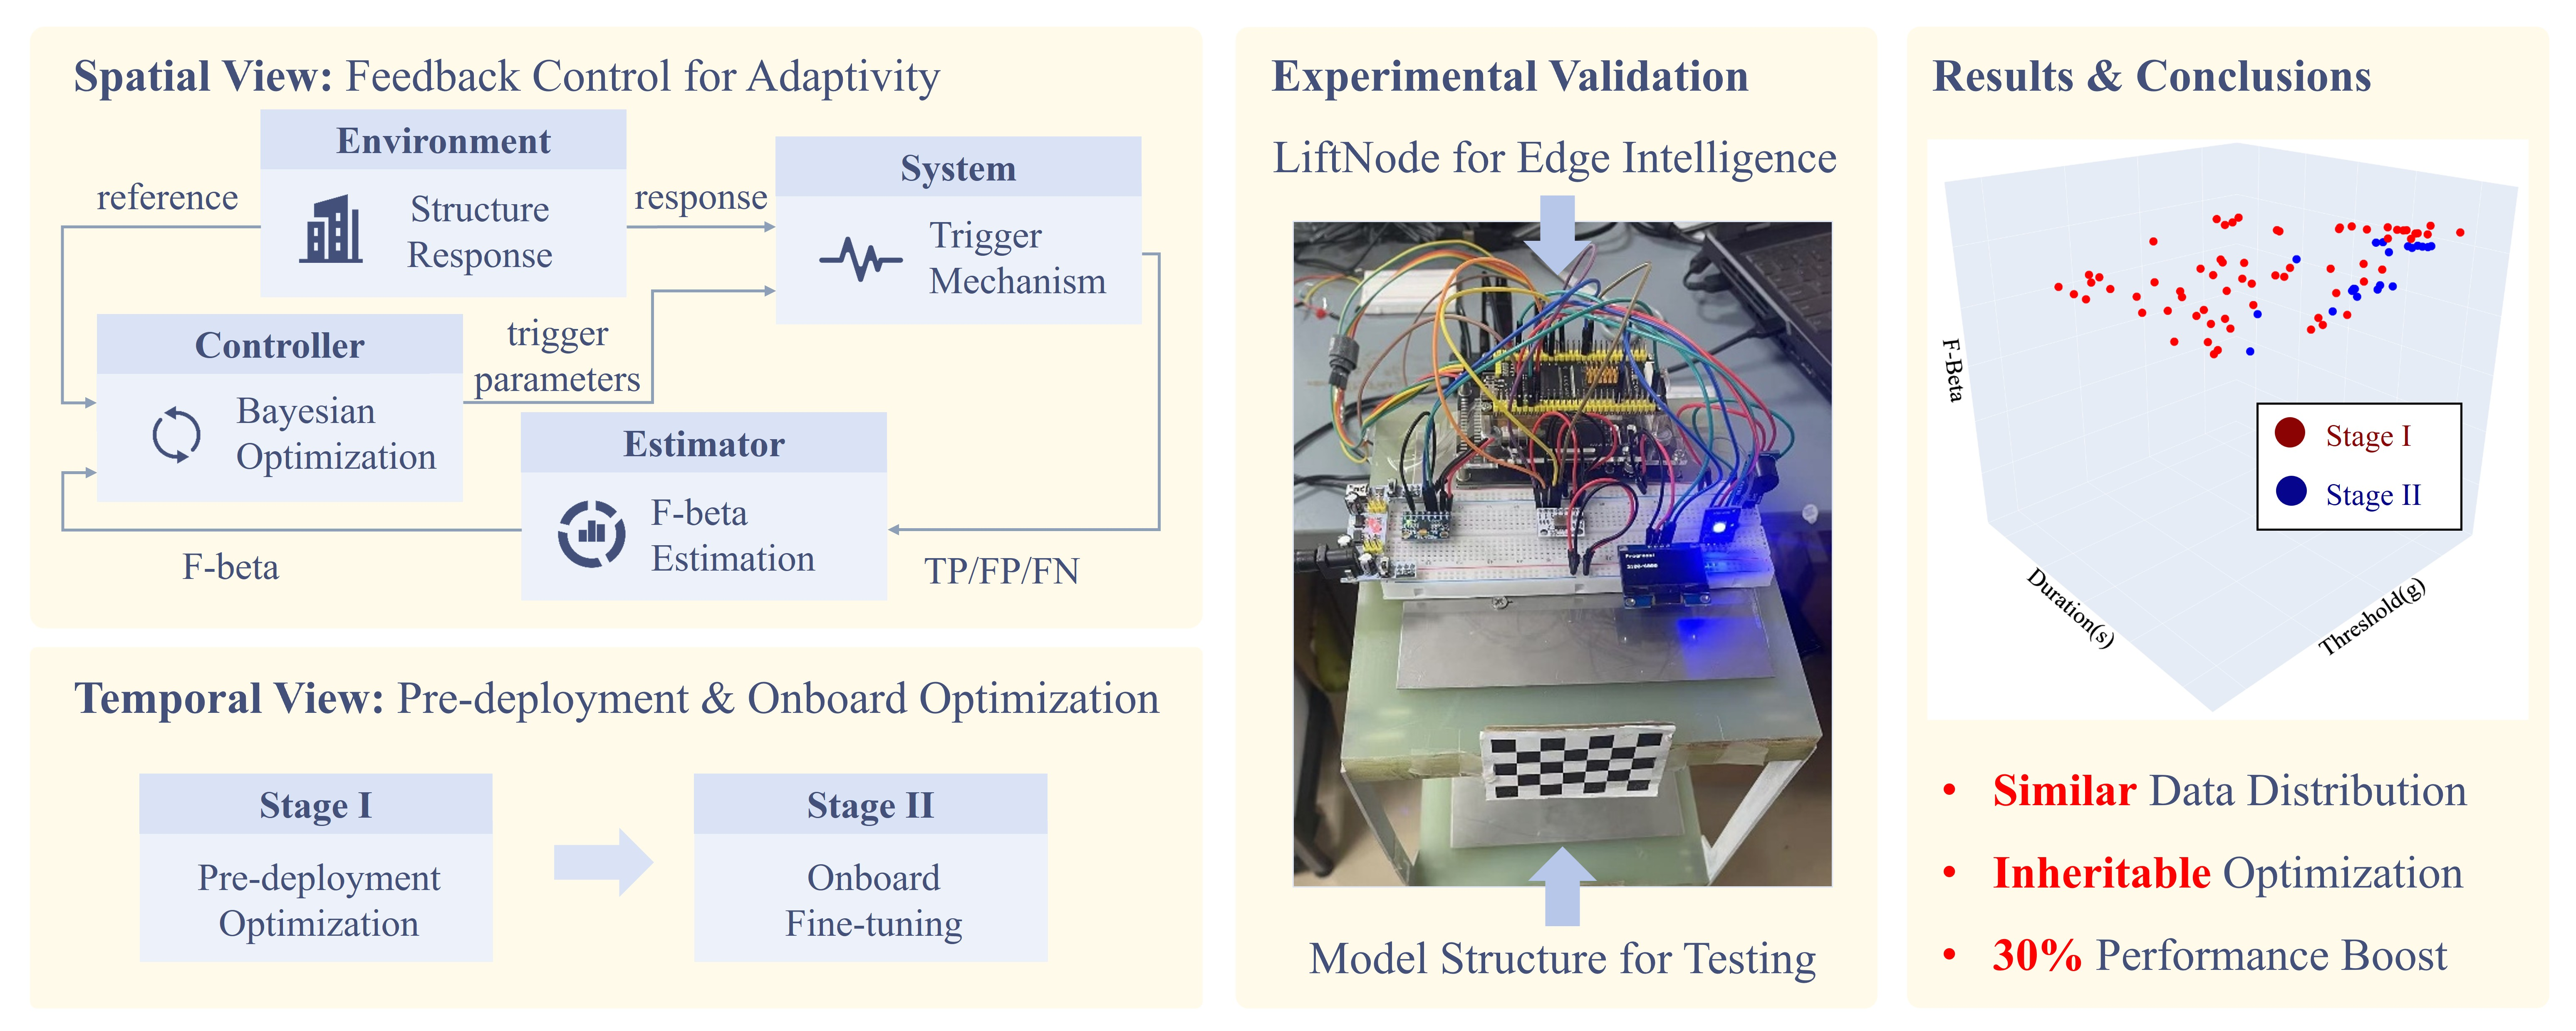
\includegraphics[width=\textwidth]{GA.jpg}
% \end{graphicalabstract}

% Research highlights
% \begin{highlights}
%   \item Adaptive feedback control for optimal trigger sensing parameters in dynamic settings.
%   \item Rapid convergence for optimal triggers with limited data via Bayesian optimization.
%   \item Onboard lightweight AI for trigger sensing to tackle partial observability.
%   \item 30\% $F_{\beta}$ performance boost for trigger sensing over conventional empirical solutions.
% \end{highlights}

% Keywords
% Each keyword is seperated by \sep
\begin{keywords}
  Structural Health Monitoring \sep 
  Edge Intelligence \sep 
  Trigger Sensing \sep
  Energy Efficiency \sep
  Feedback Control \sep 
  Bayesian Optimization \sep
  Digital Twin \sep
\end{keywords}

\maketitle

% Main text
\section{Introduction}
\label{sec:intro}

The convergence of Structural Health Monitoring (SHM) and the Internet of Things (IoT) has revolutionized infrastructure management, enabling real-time monitoring of critical assets such as buildings, bridges, and tunnels \citep{yu_recent_2023}. However, real-world deployment often faces significant constraints, particularly in remote or inaccessible locations lacking stable power supplies \citep{fu_suddenevent_2019}. As a result, many SHM systems rely on battery-powered sensor nodes to operate autonomously and wirelessly over extended periods \citep{lea_iot_2020}. This reliance introduces a critical challenge: frequent battery replacements are labor-intensive, while energy harvesting to recharge batteries is not stable. Therefore, optimizing power consumption and enhancing energy efficiency becomes essential for prolonging battery life, minimizing maintenance demands, and ensuring the consistent functionality of IoT-enabled wireless SHM systems \citep{fu_sudden_2018, laflamme_roadmap_2023}.

\begin{figure}[htbp]
    \centering
    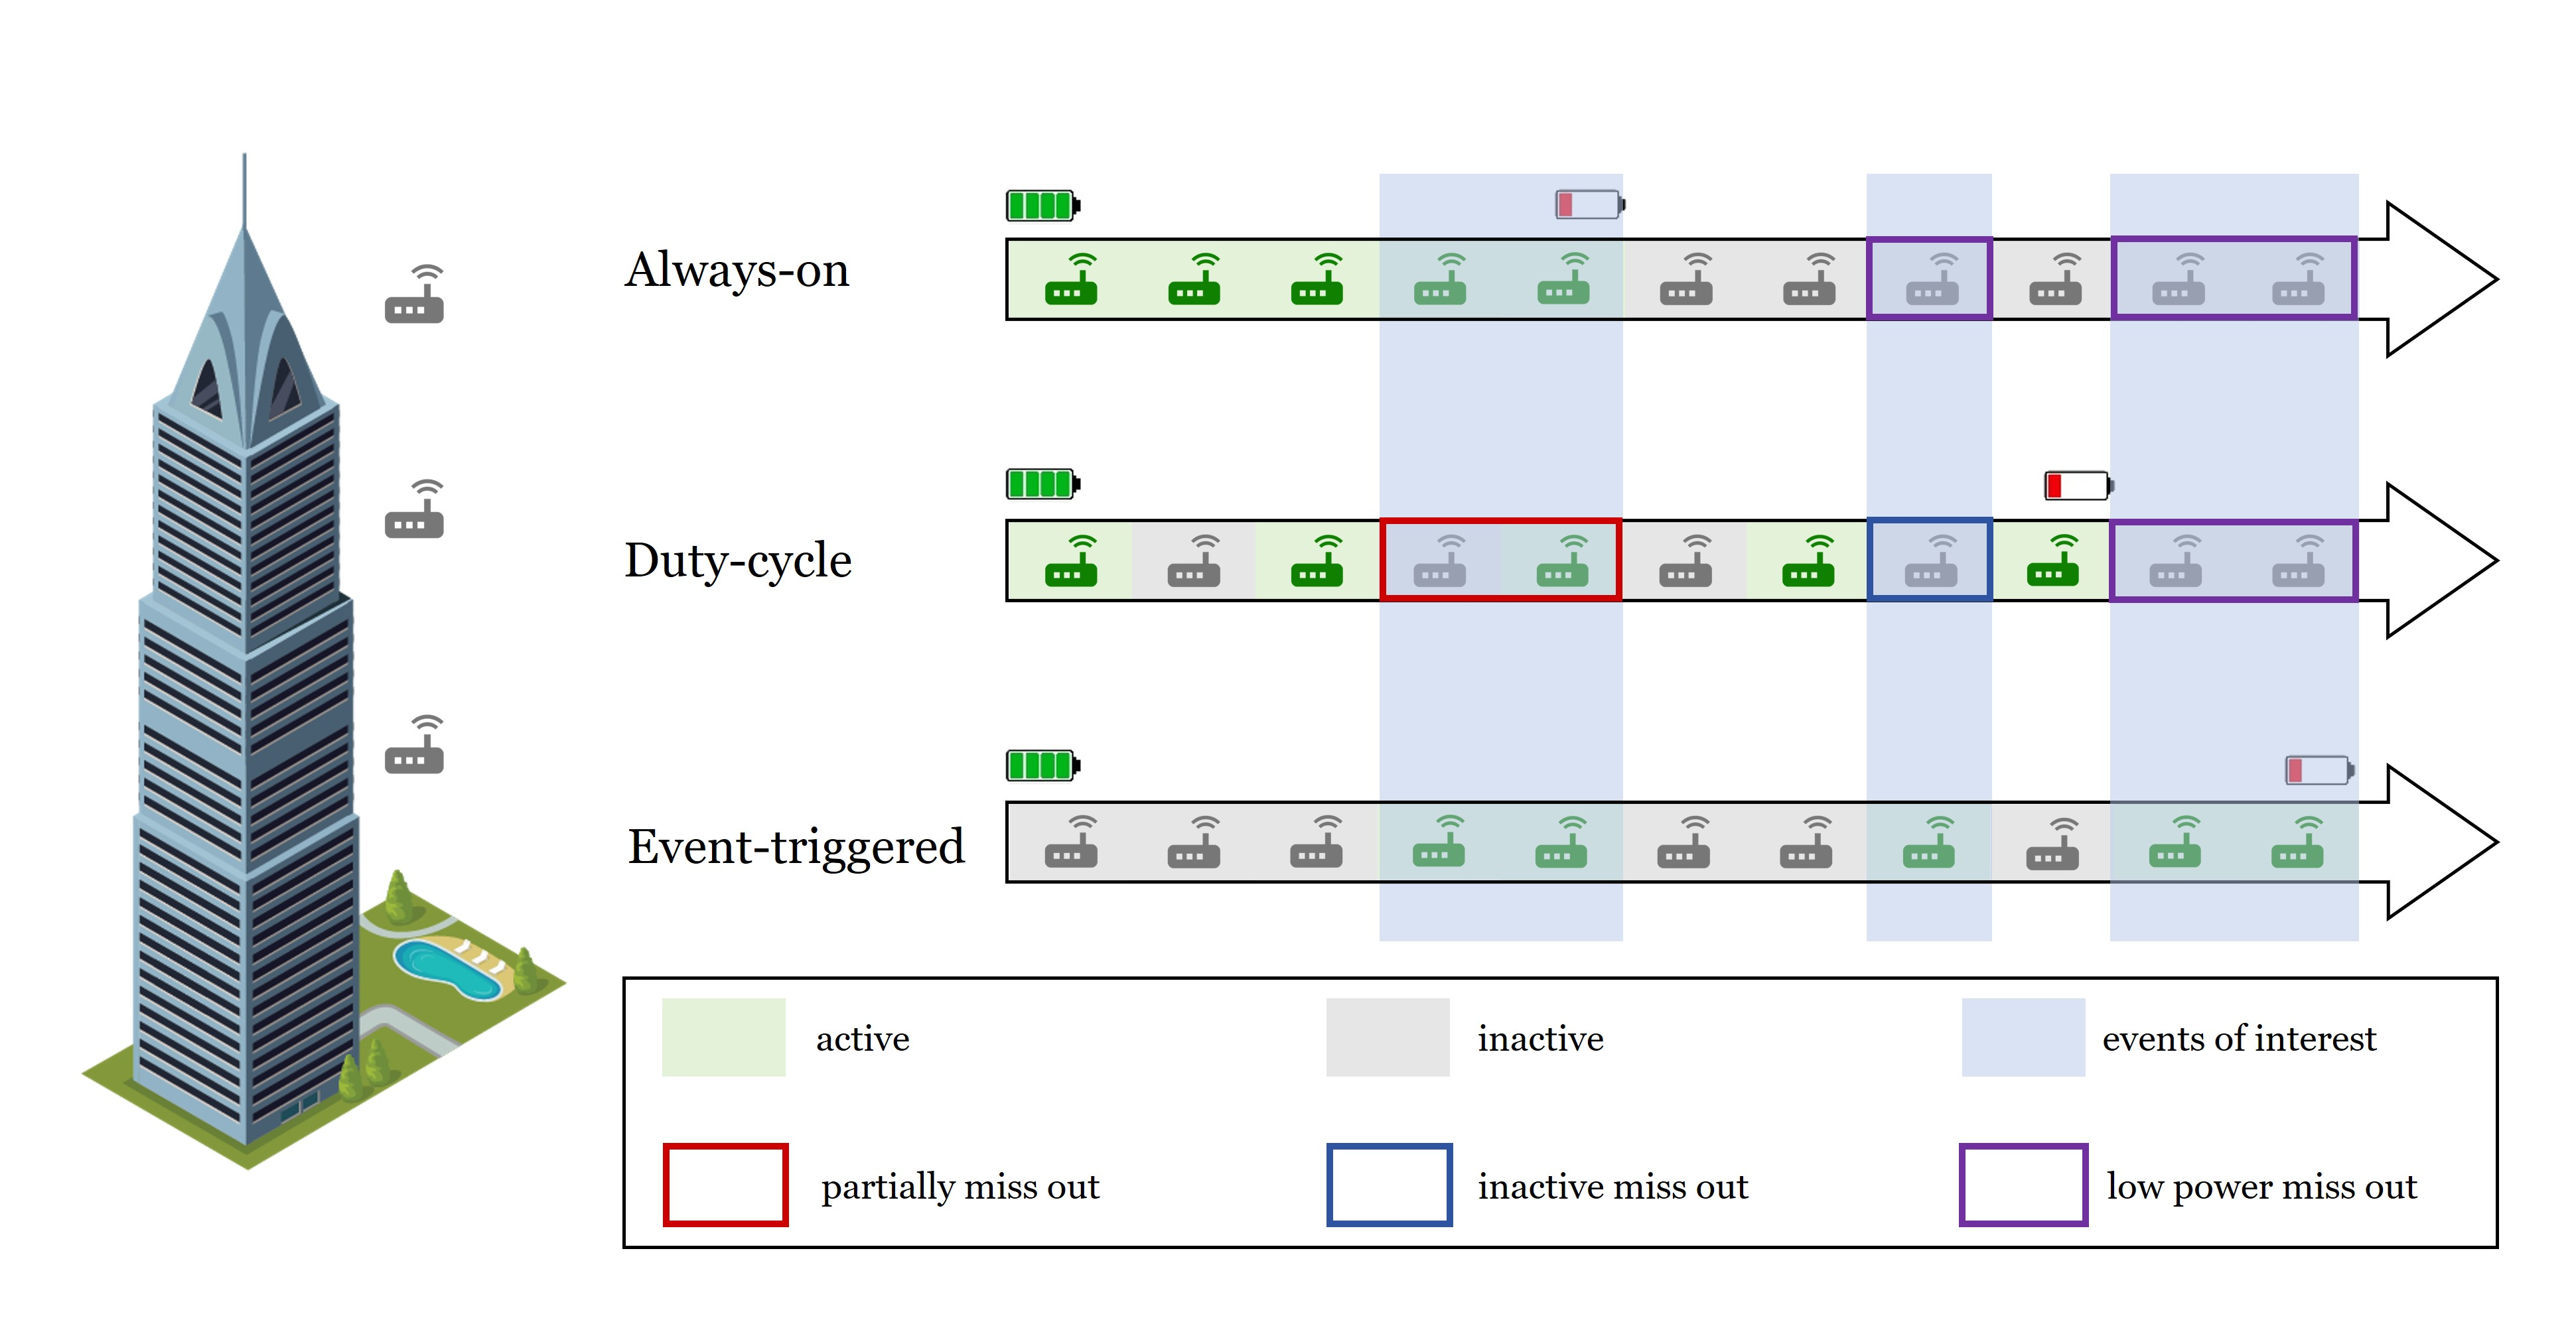
\includegraphics[width=0.85\linewidth]{Fig1.jpg}
    \caption{Schematic illustration of different sensing schemes: always on scheme quickly depletes battery; duty-cycle scheme may miss events of interest; event-triggered scheme outperforms both above schemes.}
    \label{fig:Sensing Schemes}
\end{figure}

To conserve power and extend the operational life of sensor nodes, various sensing schemes have been developed, as shown in Figure \ref{fig:Sensing Schemes}, each with distinct trade-offs \citep{fu_suddenevent_2019, ni_sensor_2023, fanariotis_reducingpowerconsumption_2024}. The always-on scheme, where sensors remain continuously active, ensures no event is missed but is only viable for systems with stable and abundant power supplies; for battery-powered devices, it rapidly depletes energy reserves. To overcome this limitation, the duty-cycling scheme alternates sensors between active and sleep modes in predefined cycles, significantly reducing power consumption and extending battery life. While simple in structure and logic, this approach risks missing critical sudden events during sleep periods, limiting its applicability in dynamic monitoring scenarios. The event-triggered scheme addresses these shortcomings by keeping sensors in a low-power state until specific conditions activate them, allowing for efficient data capture only when necessary \citep{sarwar_multimetric_2020, fu_distributed_2024}. Although it may introduce hardware and software complexity, this sensing scheme is well justified by substantial gains in energy efficiency \citep{fu_suddenevent_2019, fu_effectivestructuralimpact_2025}.

\begin{figure}[htbp]
    \centering
    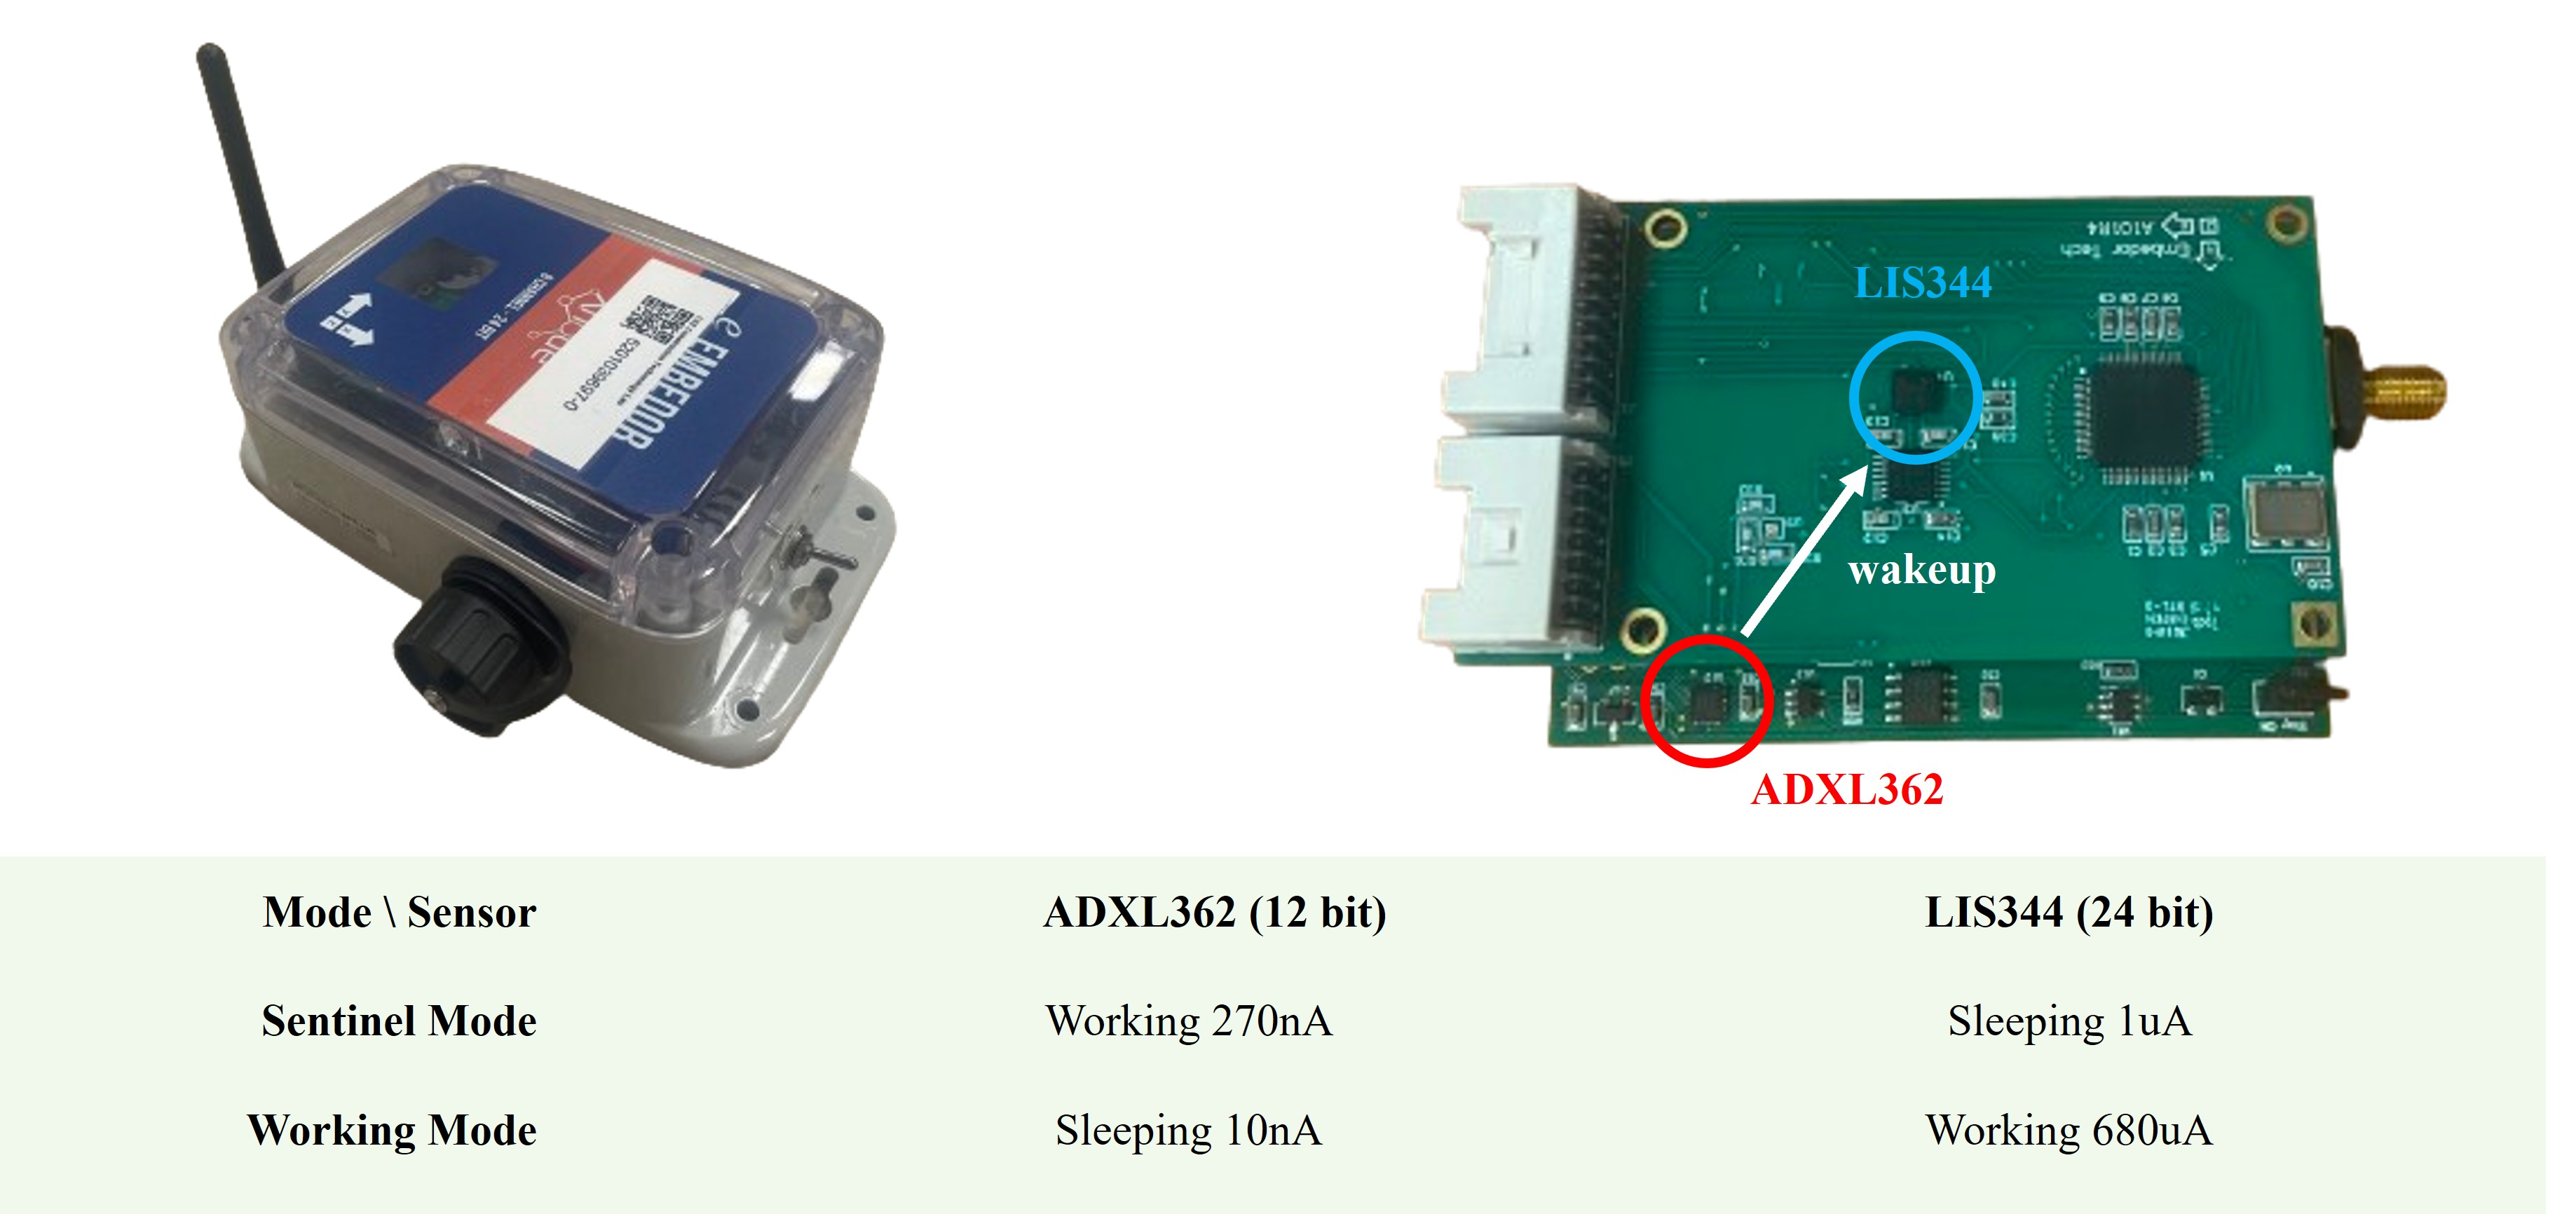
\includegraphics[width=0.85\linewidth]{Fig2.jpg}
    \caption{The sensor combination on Xnode \citep{fu_suddenevent_2019}.}
    \label{fig:Xnode Sensor Combination}
\end{figure}

Among the three sensing schemes, event-triggered sensing stands out as the most agile and energy-efficient solution for battery-powered wireless SHM systems. However, its implementation is inherently more complex \citep{ge_dynamic_2020, sarwar_multimetric_2020}. Taking the Xnode \citep{fu_suddenevent_2019} as an example, event-triggered sensing typically relies on the coordinated operation of two sensors: a low-power, low-resolution sensor and a high-power, high-resolution sensor, both capable of switching between sleep and active modes, as shown in Figure \ref{fig:Xnode Sensor Combination}. The low-power sensor acts as a sentinel, continuously monitoring for potential events of interest, while the high-power sensor is reserved for capturing detailed high-fidelity data when such events are detected. These sensor nodes operate in two modes: sentinel mode and active mode. In sentinel mode, the low-power sensor remains active to detect events, while the entire sensor node is in deep sleep mode, consuming minimal energy. Upon detecting an event, it wakes the sensor node and activates the high-power sensor, transitioning the system to active mode to record detailed information about the event. This collaborative approach effectively achieves both detection accuracy and energy efficiency, making it a pivotal innovation in modern event-triggered sensing systems for SHM applications \citep{fu_suddenevent_2019,sarwar_multimetric_2020}.

The effectiveness of event-triggered sensing relies heavily on the event detection capabilities of low-power, low-resolution sensors, such as the ADXL362 \citep{fu_suddenevent_2019,sarwar_multimetric_2020}. These sensors use pre-defined conditions, including both thresholds and duration settings to determine whether an event of interest has occurred. However, the predefined and fixed nature of these parameters inherently lacks adaptivity, making it difficult to respond effectively to dynamic and complex conditions in real-world monitoring environments \citep{zhu_eventtriggered_2022}. Without the ability to adjust to varying environmental factors, fixed threshold and duration mechanisms can result in frequent false triggers (i.e., false positives) or missed events (i.e., false negatives), significantly undermining the accuracy and reliability of wireless SHM systems \citep{fu_sudden_2018,fu_suddenevent_2019, fu_ximpact_2022}. The key challenge, therefore, lies in developing an intelligent event-triggered sensing mechanism capable of dynamically adjusting its detection settings based on changing environmental conditions. Such a mechanism must strike an ideal optimization to achieve high accuracy and maintain low power consumption. More specifically, the challenge is to minimize missed detections while keeping the false trigger rate at an acceptably low level. Addressing this issue requires innovative solutions that leverage contextual awareness, adaptive optimization techniques, and edge intelligence for onboard realization to respond dynamically to environmental variations.

To this end, this study introduces a smart adaptive event-triggered sensing framework that addresses the challenge of harmonizing detection accuracy and energy efficiency in battery-powered wireless SHM systems. In particular, the framework leverages edge intelligence, where edge computing and artificial intelligence meet, to realize onboard optimization and adaptation for wireless SHM applications \citep{tu_distributed_2024}. By enabling local data processing, edge intelligence reduces communication latency, enables adaptive parameter tuning, and context-aware control, making it ideal for resource-constrained environments \citep{cui_adaptiveedgeintelligence_2025}. The key contributions of this study are summarized as follows. (1) A feedback control mechanism is proposed as the backbone of smart adaptive trigger sensing, in which Bayesian Optimization (BO) dynamically adjusts triggering conditions to simultaneously optimize detection accuracy and energy consumption. (2) Moreover, edge intelligence is achieved by developing lightweight neural networks and deploying them directly on edge devices, thereby enabling context-aware, real-time decision-making and adaptive responses in wireless SHM systems. (3) Additionally, a staged optimization strategy. A staged trigger sensing parameter optimization strategy based on Digital Twin (DT) technology is introduced. In the first stage, pre-deployment optimization leverages abundant DT data and computational resources to perform a coarse optimization; in the second stage, onboard parameter fine-tuning is conducted using limited, partially observable real-world data, substantially accelerating the overall optimization process. (4) Finally, experimental validation on the LiftNode platform, by comparison with a traditional approach, demonstrates an approximate 30\%  
$F_{\beta}$ performance boost.

The remainder of this paper is organized as follows. Section \ref{sec:related_works} reviews related work, tracing the evolution of sensing schemes and identifying key research gaps. Section \ref{sec:smart_adaptive_triggering_mechanism} introduces the proposed Smart Adaptive Triggering Mechanism (SATM), providing a detailed explanation of its core components, including the environment, system model, estimator, and controller. Section \ref{sec:edge_deployment_strategy} describes the staged deployment strategy, emphasizing the optimization processes in both pre-deployment and onboard implementation phases. Section \ref{sec:deployment_validation} presents the experimental validation results, comparing the proposed approach with traditional methods. Finally, Section \ref{sec:conclusion} concludes the paper. 

\section{Related works}
\label{sec:related_works}

\begin{figure}[htbp]
    \centering
    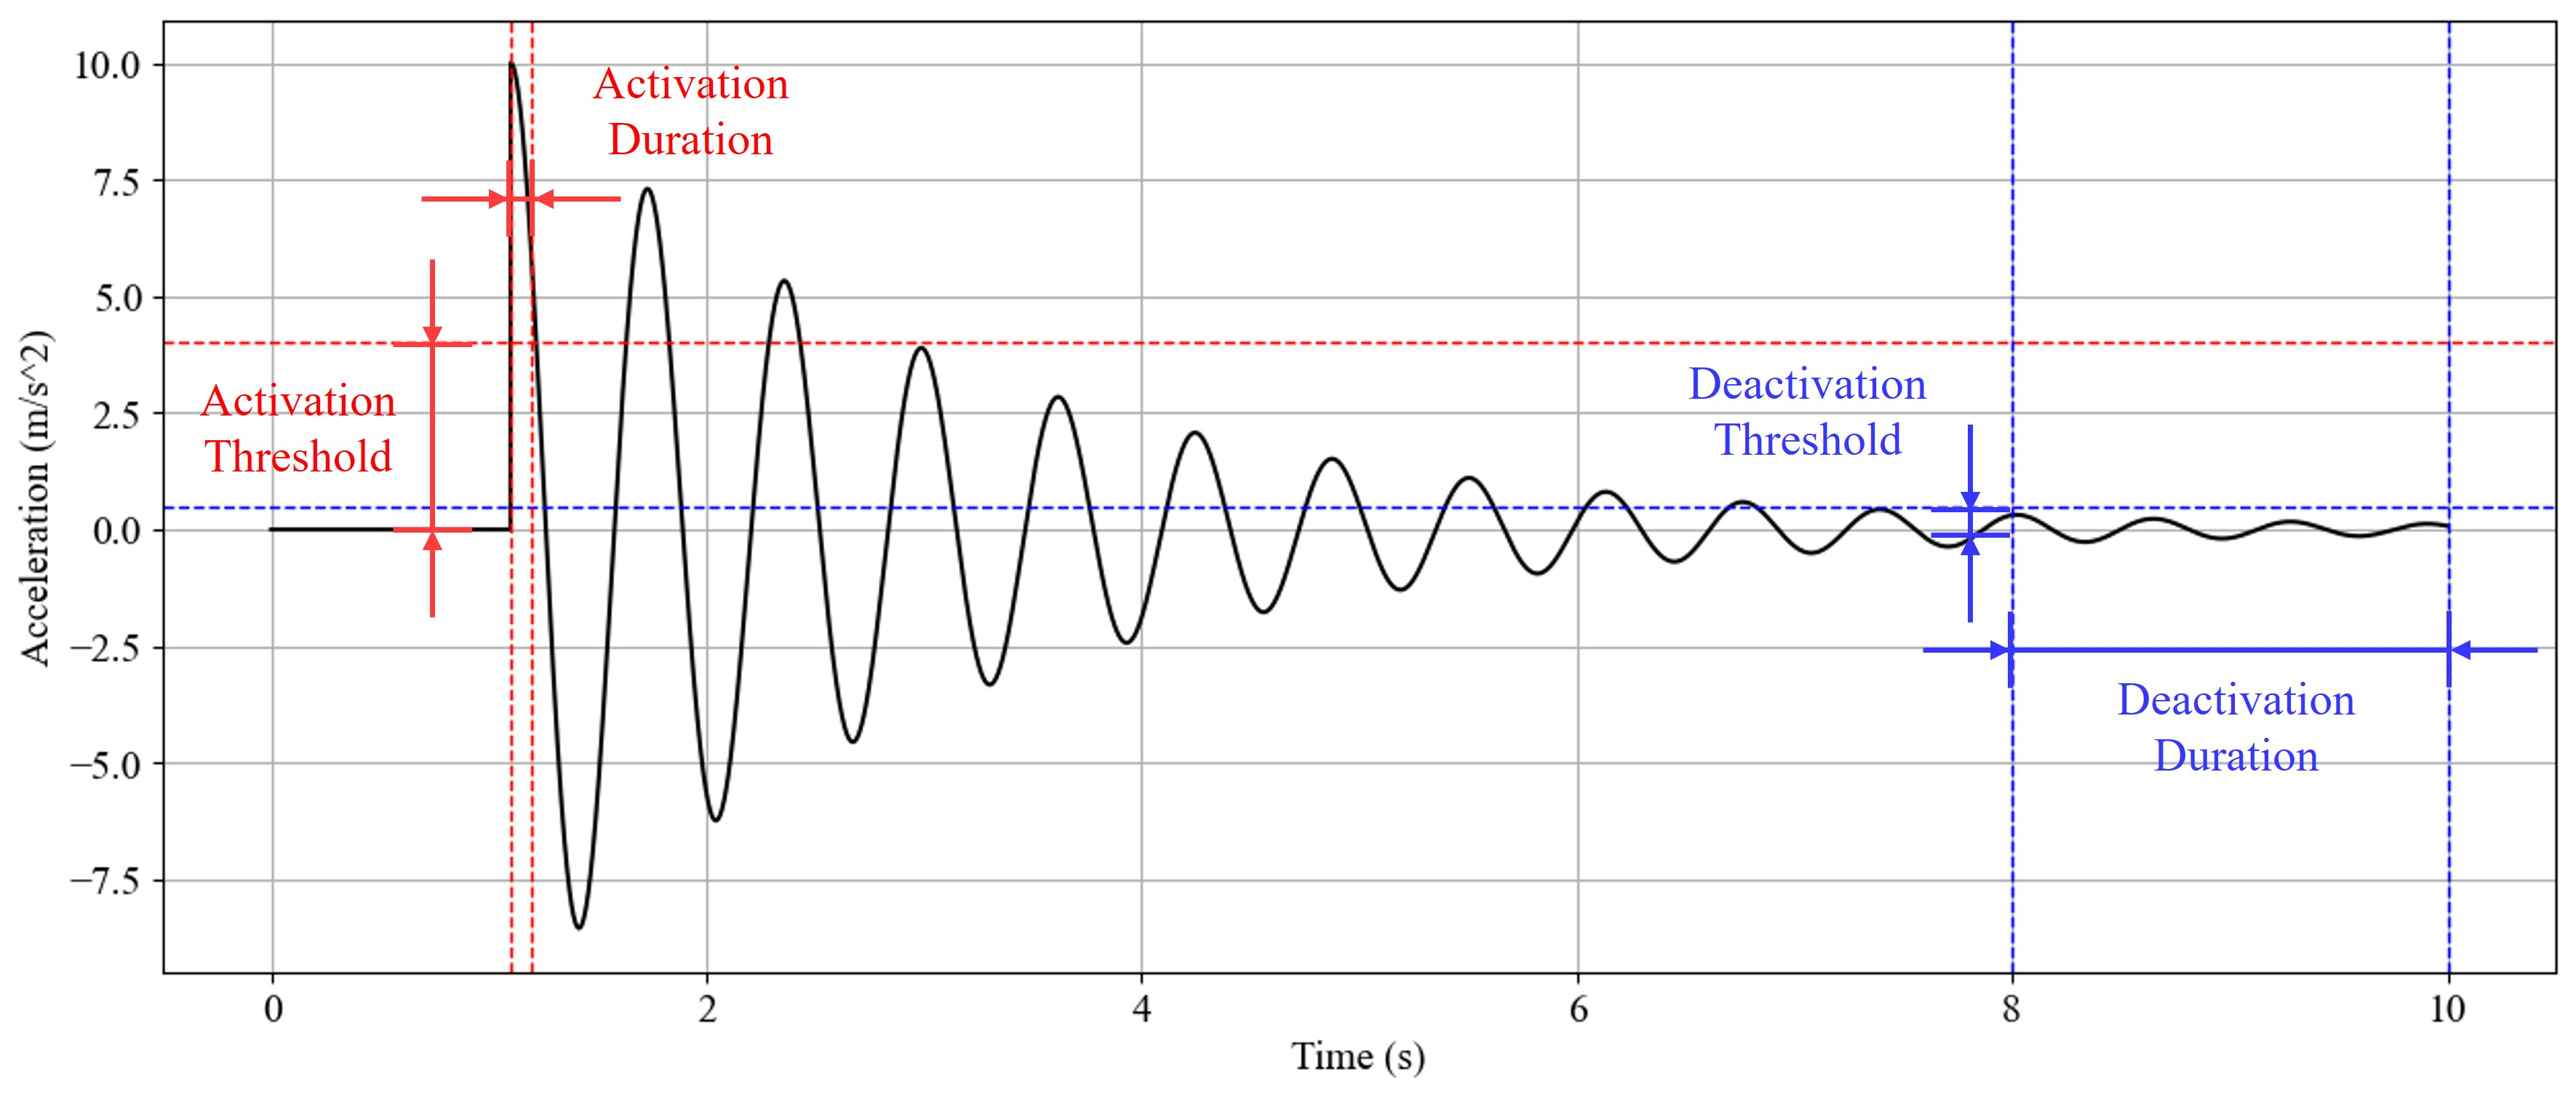
\includegraphics[width=0.85\linewidth]{Fig3.jpg}
    \caption{Schematic illustration of the trigger sensing mechanism on Xnode.}
    \label{fig:Xnode Trigger Sensing Mechanism}
\end{figure}

\subsection{Trigger sensing mechanism and its performance characterization}

Among the three different sensing schemes introduced previously, this research focuses on the trigger sensing scheme, which is widely adopted by battery-powered edge devices. As introduced in Section~\ref{sec:intro}, the trigger sensing mechanism represents a pivotal innovation in modern event-triggered sensing systems, enabling a synergy of energy efficiency and data quality. A representative example is the Xnode \citep{fu_suddenevent_2019}, which implements the trigger sensing mechanism through the combination of a low-power, low-resolution sensor and a high-power, high-resolution sensor, as illustrated in Figure~\ref{fig:Xnode Sensor Combination}. The low-power, low-resolution sensor, such as the ADXL362 \citep{analogdevices_adxl362_2024}, is responsible for motion detection by utilizing predefined thresholds and durations to determine the occurrence of an event of interest. When the signal amplitude exceeds the predefined threshold for a specified duration, an event is considered detected, and the low-power sensor activates the high-power sensor, transitioning the system into the working mode to capture detailed event data, as shown in Figure~\ref{fig:Xnode Trigger Sensing Mechanism}.

While effective, this triggering mechanism operates as a hardware-level function embedded within the sensor component itself, offering limited flexibility for software-level modifications. Higher-level system functions are thus both enabled and constrained by this implementation. In practical applications, fixed triggering parameters often lead to frequent false triggers or missed events, significantly compromising the monitoring system's accuracy and reliability. To address this limitation, a common approach involves conducting pioneer sensing to gain environmental insights and manually configuring the triggering parameters \citep{fu_suddenevent_2019}. However, this method is both time-consuming and labor-intensive, and it still fails to guarantee optimal performance. Hence, this research aims to develop an intelligent, adaptive triggering mechanism capable of dynamically adjusting the triggering parameters based on contextual insights, achieving optimal energy efficiency while maintaining high detection accuracy.

\begin{figure}[htbp]
    \centering
    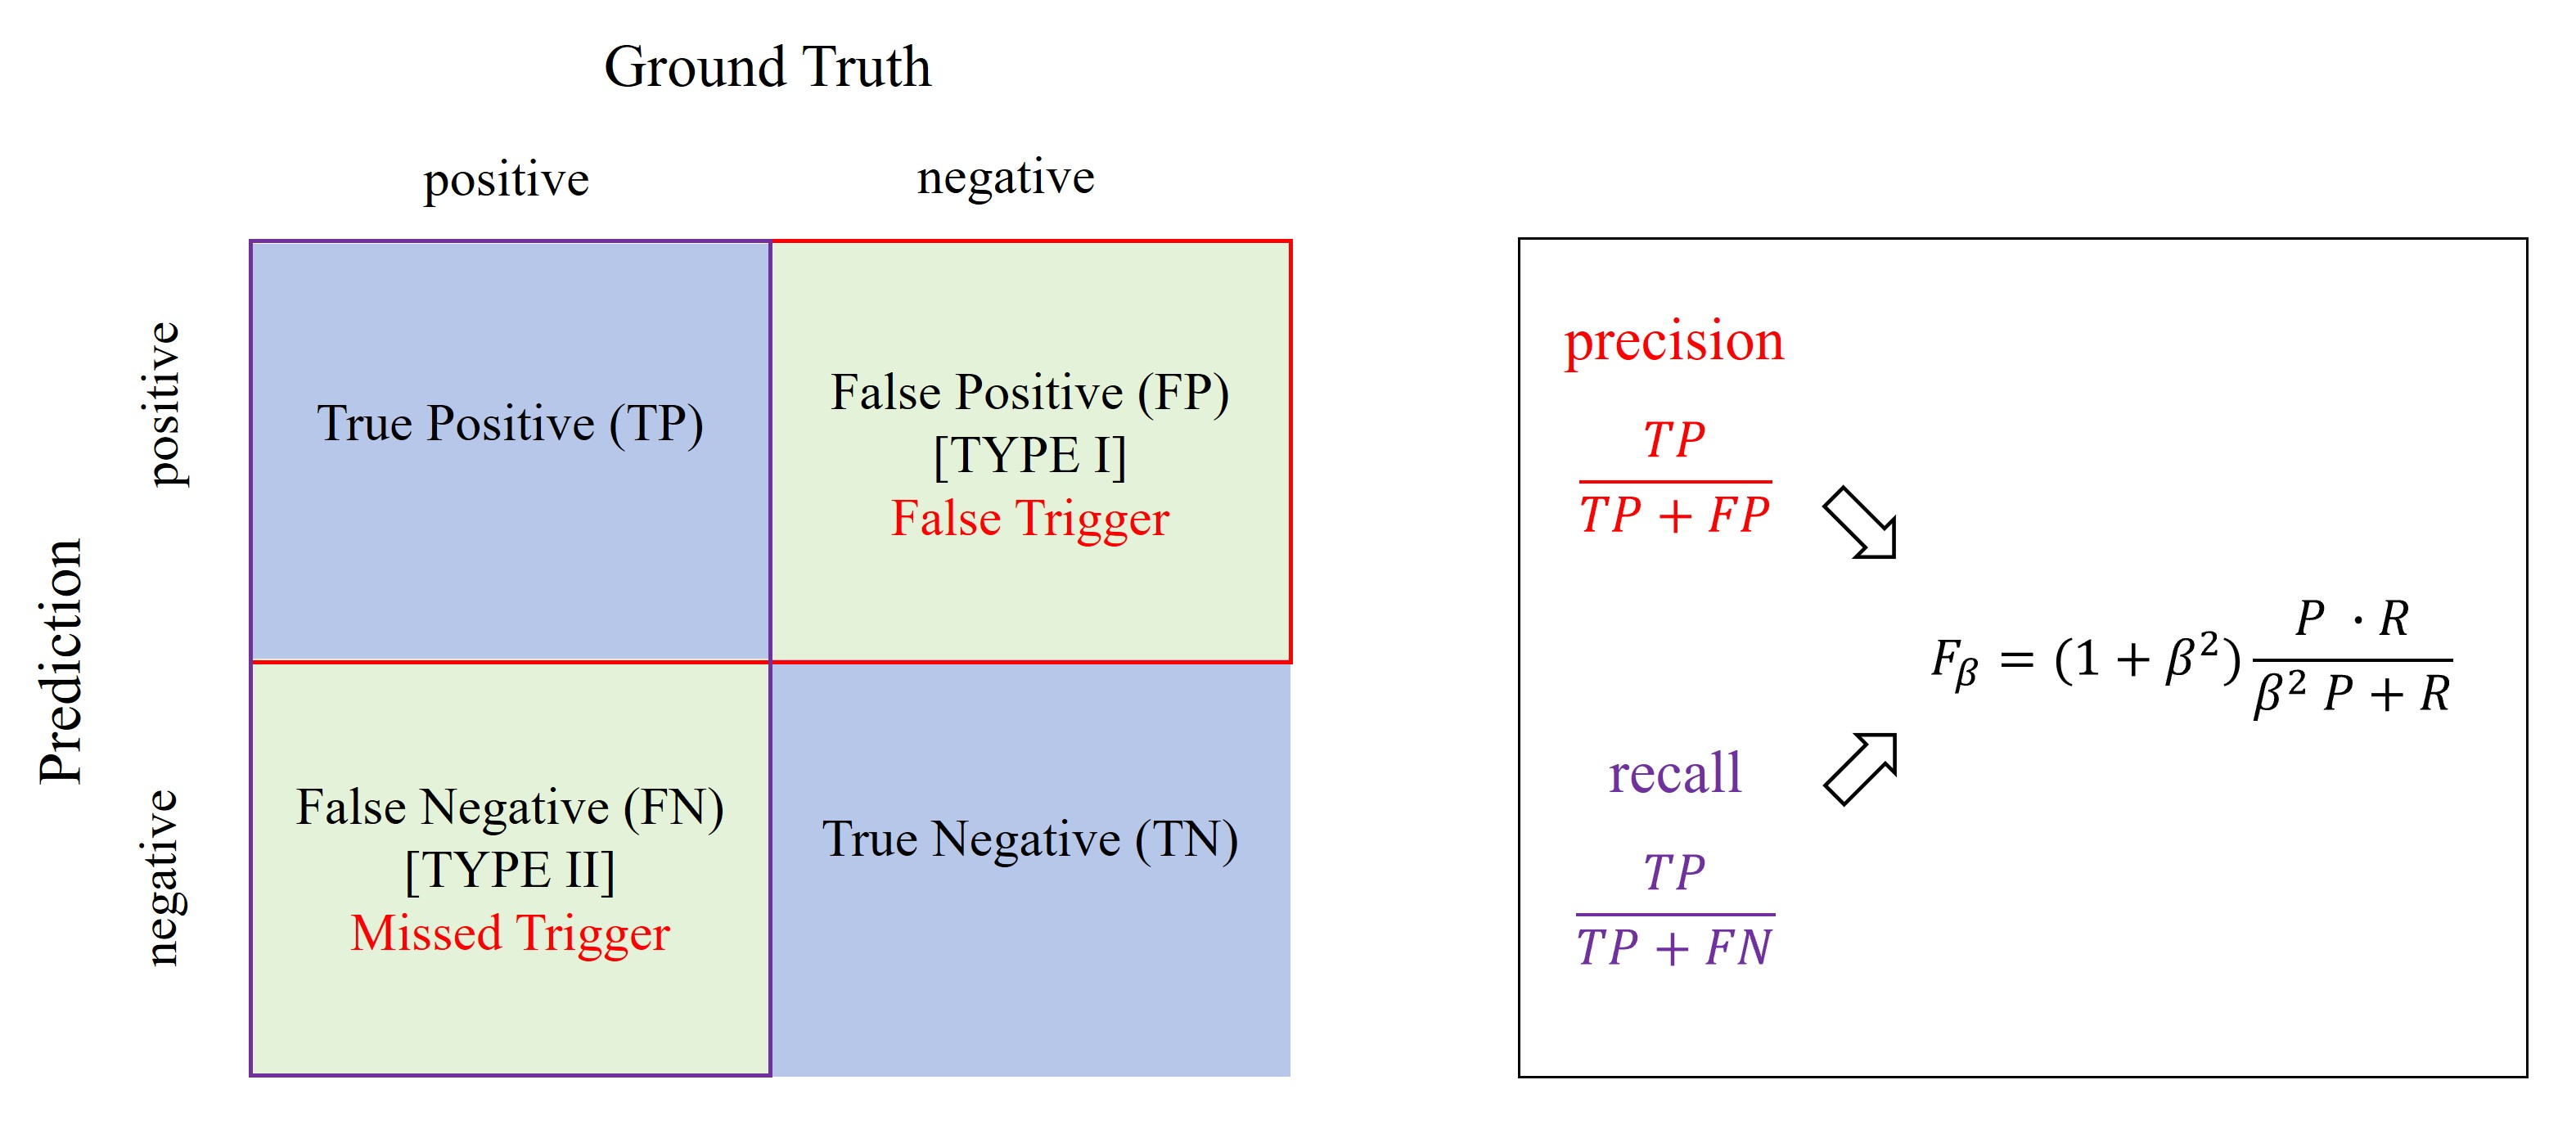
\includegraphics[width=0.85\linewidth]{Fig4.jpg}
    \caption{Schematic illustration of the confusion matrix and the $F_{\beta}$ score.}
    \label{fig:Performance Characterization}
\end{figure}

To systematically evaluate the performance of this triggering mechanism, its functionality is characterized within a mathematical framework. The mechanism essentially functions as a binary classifier, where the input is the vibration signal and the output is the event detection result. The performance of a binary classifier can be described using a confusion matrix \citep{bishop_deep_2024}, which consists of four elements: true positive (TP), false positive (FP), true negative (TN), and false negative (FN), as shown in Figure~\ref{fig:Performance Characterization}. In this context, the two most critical types of errors are missed triggers and false triggers, corresponding to false negatives and false positives, respectively. The missed trigger rate is closely related to recall (\(\text{recall} = \text{TP}/(\text{TP} + \text{FN})\)), while the false trigger rate corresponds to precision (\(\text{precision} = \text{TP}/(\text{TP} + \text{FP})\)). In SHM applications, the primary goal for trigger sensing is to minimize the missed trigger rate while keeping the false trigger rate at an acceptably low level. Consequently, the performance of the trigger sensing mechanism can be quantified by an index synthesizing both recall and precision. This index can be further characterized using the $F_{\beta}$ score \citep{bishop_deep_2024}, defined as:

\begin{equation}
\label{eq:F-beta}
F_{\beta} = (1 + \beta^2) \cdot \frac{\text{Precision} \cdot \text{Recall}}{\beta^2 \cdot \text{Precision} + \text{Recall}}
\end{equation}

Here, \(\beta\) is a parameter that adjusts the emphasis between recall and precision. The $F_{\beta}$ score provides a robust metric to evaluate the effectiveness of the triggering mechanism in achieving the desired balance between detection accuracy and energy efficiency. For cases recall is more important, \(\beta\) can be set to a value greater than 1, while for cases precision is more important, \(\beta\) can be set to a value less than 1. In practice, the optimal value of \(\beta\) is determined by the specific requirements of the SHM application.

\subsection{Research gaps and challenges}
\label{sec:gaps_challenges}

The primary research gap lies in the reliance of current triggering mechanisms on static thresholds and durations, which cannot adapt to dynamic environmental changes. This rigidity limits their effectiveness in evolving scenarios. Existing solutions often employ pioneer sensing to gather environmental insights and manually configure parameters \citep{fu_suddenevent_2019}. While this approach can rationalize parameter settings, it is time-consuming, labor-intensive, and relies heavily on heuristic configurations that rarely achieve global optimality. To address these limitations, an ideal adaptive mechanism should dynamically adjust triggering parameters in real-time based on environmental insights. Such a mechanism would start with a conservative configuration to ensure high recall and iteratively optimize toward a global optimum, featuring high detection accuracy and high energy efficiency while minimizing manual intervention.

Several challenges impede the design and implementation of adaptive triggering mechanisms. (1) The first challenge is the inherent lack of adaptivity in current systems, which depend on fixed parameters—such as predefined thresholds and durations—that restrict their robustness and applicability in dynamic environments. (2) The second challenge involves data unobservability and uncertainty. In real-world deployments, some data cannot be fully observed; for example, events that fail to trigger data collection are never recorded and thus cannot be analyzed further. Moreover, certain data may not be collected at all (e.g., the ground truth label of an event type), while other data may exhibit high uncertainty during collection (e.g., the distribution of events such as earthquakes). (3) The third challenge is the high observation cost, as the computation of metrics like the \(F_{\beta}\) score requires extensive data collection and processing, thereby imposing substantial time and computational overheads on resource-constrained edge devices.

\subsection{Potential enablers}

Building upon the analysis of the research gaps and challenges, several key enablers can be synthesized into a cohesive solution for a smart adaptive triggering mechanism, including (1) feedback control, (2) Bayesian Optimization (BO), (3) digital twin technology, and (4) edge intelligence. Together, these enablers can address the major challenges introduced in Section \ref{sec:gaps_challenges}.

Feedback control \citep{ogata_modern_2010} can serve as the cornerstone of adaptivity by incorporating the \(F_{\beta}\) score into its feedback loop, directly addressing Challenge 1. This integration can unify recall and precision into a single optimization metric, thereby transforming a multi-objective optimization problem into a single-objective one. Complementing this, Bayesian Optimization \citep{agrawal_bayesianoptimization_2021} can act as the engine to power feedback control. By leveraging surrogate models and iterative updates, BO can efficiently guide parameter adjustments, effectively handle black-box problems, and reduce observation costs in resource-constrained environments, making it a promising solution to Challenge 3. To enhance the performance of the adaptive triggering, digital twin technology \citep{ganguli_digitaltwindynamic_2023} and edge intelligence \citep{lea_iot_2020} can be introduced as acceleration engines. Digital twin technology can enable controlled data augmentation through the generation of synthetic datasets, mitigating issues such as unknown event distributions (as mentioned in Challenge 2) and substantially lowering real-world optimization costs (as mentioned in Challenge 3) by facilitating iterative computations in virtual environments. Meanwhile, edge intelligence can be realized by deploying lightweight neural networks directly on edge devices, which can allow for real-time ground truth estimation and the inference of unobservable data (e.g., missed events) as mentioned in Challenge 2, further enhancing system adaptability and efficiency.

\section{Smart adaptive triggering mechanism}
\label{sec:smart_adaptive_triggering_mechanism}

\begin{figure}[htbp]
    \centering
    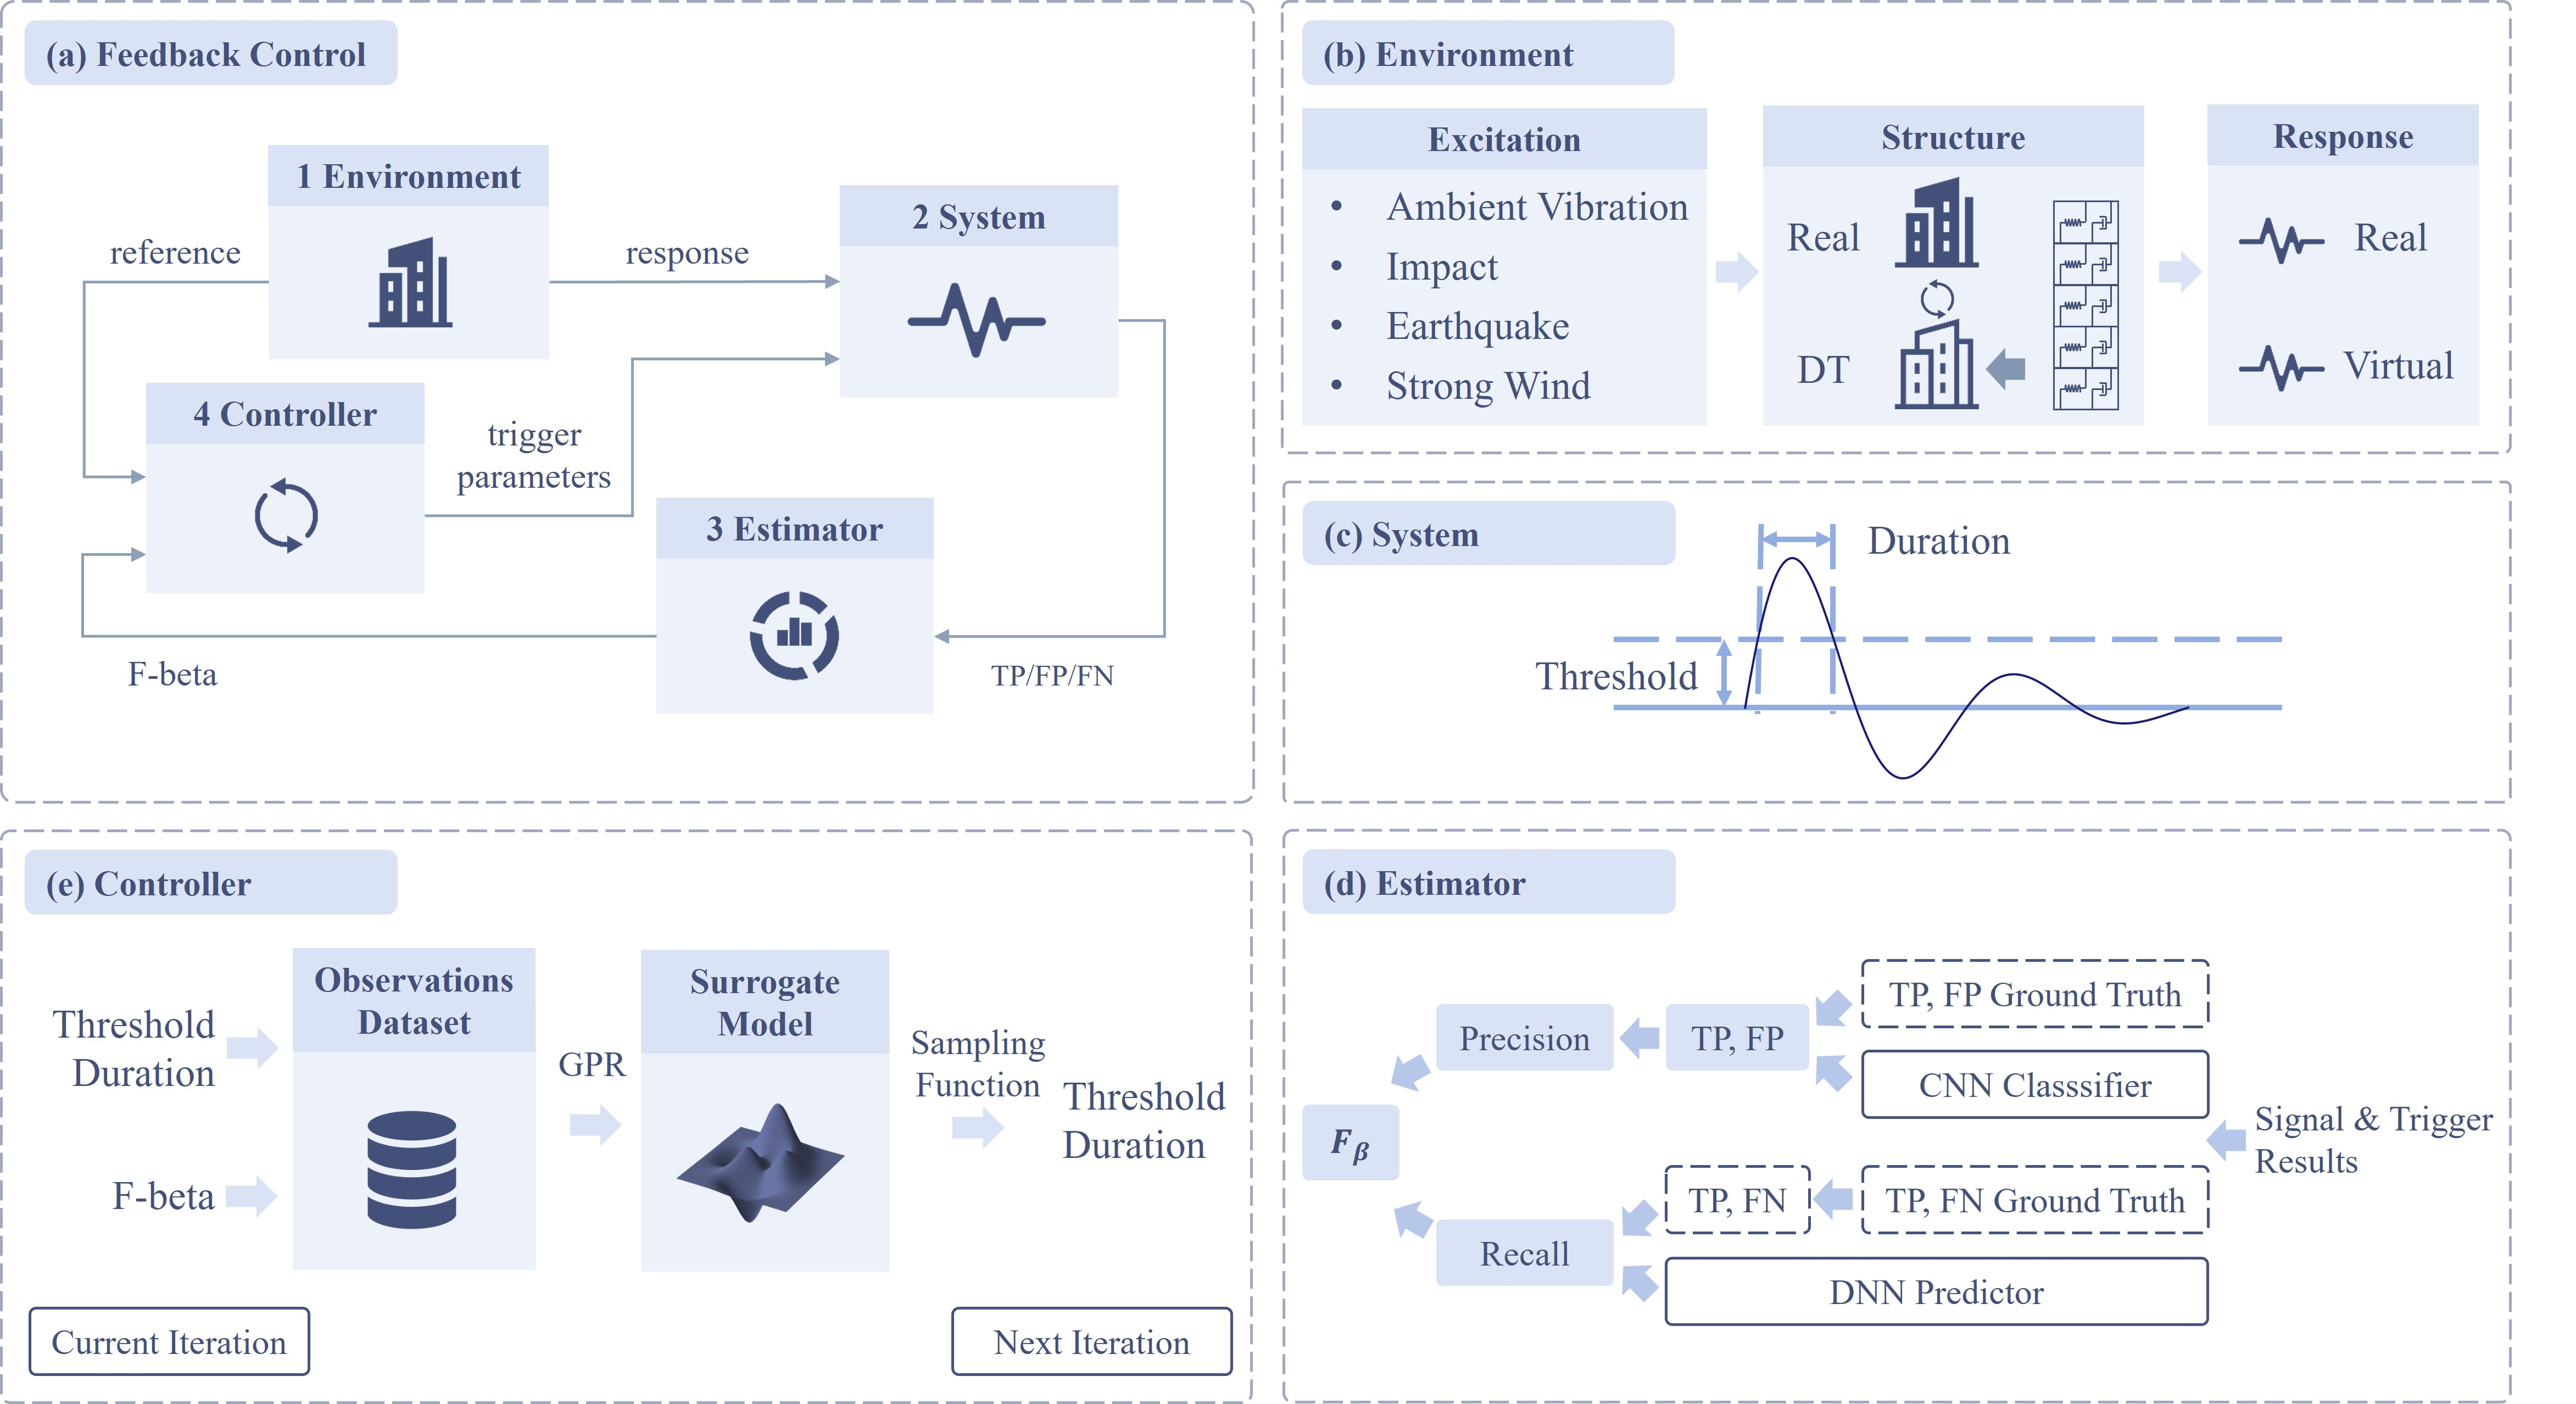
\includegraphics[width=\linewidth]{Fig5.jpg}
    \caption{Feedback control for adaptive triggering mechanism.}
    \label{fig:SATM}
\end{figure}

As depicted in Figure \ref{fig:SATM}, this study introduces a smart adaptive triggering mechanism that integrates multiple enabling technologies to address the inherent challenges outlined in Section \ref{sec:related_works}. This section begins with an overview of the proposed mechanism, followed by a detailed discussion of its constituent components.

\subsection{Overview}

The proposed SATM employs feedback control as its backbone, serving as the key mechanism for adaptive optimization toward global optimal configurations. A feedback control loop typically consists of four major components: the environment, the system model, the estimator, and the controller \citep{ogata_modern_2010}, as illustrated in Figure \ref{fig:SATM} (a). In the context of SHM and trigger sensing, the environment represents the target structure's responses to various excitations. The system component corresponds to the threshold- and duration-based triggering mechanism, which serves as the primary optimization target. The estimator assesses the system's performance, providing essential feedback to guide adjustments. Lastly, the controller functions as the driving engine, steering the system toward its optimal configuration by addressing two critical aspects: (1) identifying the optimal state and (2) determining the pathway to achieve it.

\subsection{The environment}
\label{component-environment}

The environment component is characterized in relation to the system component and serves as the source of input signals for the system in trigger sensing for SHM. Specifically, it represents the structural responses generated by external excitations. As illustrated in Figure \ref{fig:SATM} (b), the environment component comprises three interconnected elements: (1) excitations, (2) structures, and (3) responses. In practical applications, responses are typically collected directly by sensors. However, to leverage the advantages of digital twin technology, this section focuses on constructing an effective surrogate model for the environment component. 

\subsubsection{Excitations}
\label{environment-excitations}

Excitations refer to external forces or disturbances acting on the structures, caused by various events, whether of interest or not. For the purpose of this study, four types of events are considered: (1) ambient vibration, (2) impact, (3) earthquake, and (4) strong wind. Among these, ambient vibration is categorized as an uninteresting event, while the remaining three are classified as events of interest. In engineering practice, these events often occur naturally within the environment. However, in the digital twin framework, excitation signals can be synthetically generated using computational methods to accelerate the optimization process. The technical details for signal generation can obscure the core concepts of the proposed mechanism, and thus only the key points are highlighted below. 

Firstly, ambient vibration refers to environmental noise, which can be modeled as Gaussian white noise characterized by its mean value and standard deviation. It acts on every degree of freedom of the structure, representing the background noise present in the monitoring environment. Secondly, impact events can be modeled as single impulse signals with predefined amplitude and duration. In practice, these signals represent spike-like forces caused by sudden external disturbances acting on the structure. For simulation purposes, impacts can be applied to a random degree of freedom with random amplitude and direction for a very short duration. Thirdly, earthquakes can be modeled as the superposition of multiple sinusoidal waves with varying frequencies, amplitudes, and phases. These signals should first be modulated in the frequency domain to align with the power spectral density of real earthquake data, then further modulated in the time domain to generate time-history signals. The forces can be applied at the ground level and distributed across the structure’s degrees of freedom using a predefined force distribution matrix. Fourthly, strong wind can first be modeled based on wind pressure distribution acting on the structure and then equivalently converted into concentrated forces applied to the structure’s mass points. In addition to frequency domain modulation, time domain modulation can be applied to capture the temporal evolution of wind forces. Most importantly, the spatial interrelation between different points on the structure should be considered to accurately represent the complex nature of wind loading.

\subsubsection{Structures}
\label{environment-structures}

Structures represent the physical systems being monitored, serving as both the targets of excitations and the sources of responses. Acting as intermediaries between excitations and responses, the dynamic behaviors of structures govern how they react to various external forces. These behaviors are typically characterized by the equation of motion, which, for an $n$-degree-of-freedom system, is expressed as:

\begin{equation}
    \mathbf{M} \ddot{\mathbf{x}}(t) + \mathbf{C} \dot{\mathbf{x}}(t) + \mathbf{K} \mathbf{x}(t) = \mathbf{G} \mathbf{P}(t),
\end{equation}

where $\mathbf{M} \in \mathbb{R}^{n \times n}$, $\mathbf{C} \in \mathbb{R}^{n \times n}$, and $\mathbf{K} \in \mathbb{R}^{n \times n}$ are the mass, damping, and stiffness matrices, respectively; $\mathbf{x}(t) \in \mathbb{R}^{n}$ is the displacement vector; $\dot{\mathbf{x}}(t)$ and $\ddot{\mathbf{x}}(t)$ represent the velocity and acceleration vectors, respectively. On the right-hand side, $\mathbf{G} \in \mathbb{R}^{n \times m}$ is the force distribution matrix, and $\mathbf{P}(t) \in \mathbb{R}^{m}$ is the time-dependent force vector representing excitations acting on the structure. In this study, for simplicity, it is assumed that $m = n$, meaning that each degree of freedom has a corresponding input force. For numerical analysis and simulation, the equation of motion can be reformulated into a state-space representation to facilitate computation and control analysis \citep{newmark_methodcomputationstructural_1959}. 

\subsubsection{Responses}
\label{environment-responses}

Responses are signals generated by the dynamic interaction of excitations and structures, representing structural behaviors under external forces. These signals, whether real (from physical environments) or virtual (from digital twins), serve as the critical input to the system component for detecting events of interest. A widely used method for simulating structural responses is the Newmark-beta method \citep{newmark_methodcomputationstructural_1959}, which is an iterative numerical integration scheme for solving the equation of motion in structural dynamics. The algorithmic process is summarized as Algorithm \ref{alg:newmark-beta}.

\begin{algorithm}[H]
    \caption{Newmark-beta Method for Structural Response Simulation \citep{newmark_methodcomputationstructural_1959}}
    \label{alg:newmark-beta}
    \begin{algorithmic}[1]
    \STATE Input: mass matrix $\mathbf{M}$, 
    damping matrix $\mathbf{C}$, 
    stiffness matrix $\mathbf{K}$, 
    force distribution matrix $\mathbf{G}$, 
    external force $\mathbf{P}(t)$, 
    initial displacement $\mathbf{x}_0$, 
    initial velocity $\dot{\mathbf{x}}_0$, 
    initial acceleration $\ddot{\mathbf{x}}_0$, 
    time step $\Delta t$, 
    integration parameters $\beta$, $\gamma$ (typically set to 0.25 and 0.5, respectively)
    \STATE Output: displacement $\mathbf{x}_t$, velocity $\dot{\mathbf{x}}_t$, acceleration $\ddot{\mathbf{x}}_t$
    \STATE \textbf{Initialization:}
    \STATE Compute helper coefficients: $a_0 = 1 / (\beta \Delta t^2)$, $a_1 = \gamma / (\beta \Delta t)$, $a_2 = 1 / (\beta \Delta t)$, $a_3 = 1 / (2 \beta) - 1, a_4 = \gamma / \beta - 1, a_5 = \Delta t / 2(\gamma / \beta - 2), a_6 = \Delta t (1 - \gamma), a_7 = \gamma \Delta t$
    \STATE Compute effective stiffness matrix: $ \mathbf{K}^e = \mathbf{K} + a_1 \mathbf{C} + a_0 \mathbf{M} $
    \STATE $\mathbf{x} \gets \mathbf{x}_0$, $\dot{\mathbf{x}} \gets \dot{\mathbf{x}}_0$, $\ddot{\mathbf{x}} \gets \ddot{\mathbf{x}}_0$
    \STATE \textbf{Iteration:}
    \FOR{each time step $t = 1$ to $T$}
        \STATE Compute effective force: $\mathbf{G} \mathbf{P}_{t+\Delta t}^e = \mathbf{G} \mathbf{P}_{t+\Delta t} + (a_0 \mathbf{x}_t + a_2 \dot{\mathbf{x}}_t + a_3 \ddot{\mathbf{x}}_t) \mathbf{M} + (a_1 \mathbf{x}_t + a_4 \dot{\mathbf{x}}_t + a_5 \ddot{\mathbf{x}}_t) \mathbf{C}$
        \STATE Compute the displacement at $t+\Delta t$: $\mathbf{x}_{t+\Delta t} = (\mathbf{K}^{e})^{-1} \mathbf{G} \mathbf{P}_{t+\Delta t}^e$
        \STATE Compute the acceleration at $t+\Delta t$: $\ddot{\mathbf{x}}_{t+\Delta t} = a_0 (\mathbf{x}_{t+\Delta t} - \mathbf{x}_t) - a_2 \dot{\mathbf{x}}_t - a_3 \ddot{\mathbf{x}}_t$
        \STATE Compute the velocity at $t+\Delta t$: $\dot{\mathbf{x}}_{t+\Delta t} = \dot{\mathbf{x}}_t + a_6 \ddot{\mathbf{x}}_t + a_7 \ddot{\mathbf{x}}_{t+\Delta t}$
        \STATE Update current state: $\mathbf{x}_t \gets \mathbf{x}_{t+\Delta t}$, $\dot{\mathbf{x}}_t \gets \dot{\mathbf{x}}_{t+\Delta t}$, $\ddot{\mathbf{x}}_t \gets \ddot{\mathbf{x}}_{t+\Delta t}$
    \ENDFOR
    \end{algorithmic}
\end{algorithm}

\subsection{The system}
\label{component-system}

The system component refers to the threshold- and duration-based triggering mechanism, which functions as a binary classifier and serves as the primary optimization target within the feedback control loop \citep{fu_suddenevent_2019}. In practical applications, this mechanism is implemented in low-level hardware, such as the ADXL362 sensor \citep{analogdevices_adxl362_2024}, with users able to adjust its triggering parameters—thresholds and durations—via software interfaces. The threshold parameter operates within a continuous value space, whereas the duration parameter is defined in a discrete space, corresponding to an integer number of sampling points. Complementing the triggering mechanism is a deactivation mechanism, as shown in Figure \ref{fig:Xnode Trigger Sensing Mechanism}, which, although outside the scope of this study, plays a critical role in real-world applications. The deactivation mechanism resets the system to sentinel mode after capturing an event, ensuring readiness for subsequent detection cycles and enabling seamless operation.

As illustrated in Figure \ref{fig:SATM} (c), the triggering mechanism relies on monitoring consecutive time steps where the signal amplitude surpasses the predefined threshold. When the count of such steps meets or exceeds the specified duration, an event is triggered, transitioning the system from sentinel mode to active mode. The underlying logic of this mechanism can be formalized in Algorithm \ref{alg:triggering_mechanism}, which serves two critical roles: first, it encapsulates the operational principles governing real hardware implementations; second, it provides the foundation for the system component within the digital twin framework, facilitating virtual testing and optimization of the triggering mechanism under diverse conditions. 

\begin{algorithm}[H]
    \caption{Threshold- and Duration-Based Triggering Mechanism}
    \label{alg:triggering_mechanism}
    \begin{algorithmic}[1]
    \STATE \textbf{Input:} signal value $s$, threshold $\tau$, duration $d$
    \STATE \textbf{Output:} trigger flag $T$ (binary: 1 for trigger, 0 for no trigger; initialized as 0)
    \STATE \textbf{Internal Variable:} counter $c$ (initialized as 0, used to track consecutive time steps)
    \STATE For each time step $t$:
        \IF{$|s| \geq \tau$} 
            \STATE Increment counter: $c \gets c + 1$
            \IF{$c \geq d$}
                \STATE Set trigger flag: $T \gets 1$
                \STATE Reset counter: $c \gets 0$
            \ENDIF
        \ELSE
            \STATE Reset counter: $c \gets 0$
            \STATE Set trigger flag: $T \gets 0$
        \ENDIF
    \end{algorithmic}
\end{algorithm}

\subsection{The estimator}
\label{component-estimator}

The estimator evaluates the system's performance using the $F_{\beta}$ score, a comprehensive metric that harmonizes recall and precision. This simplifies the optimization process by transforming a multi-objective problem into a single-objective one. The $F_{\beta}$ score, defined in Equation \ref{eq:F-beta}, adjusts the trade-off between recall and precision based on the parameter $\beta$. For SHM applications, $\beta > 1$ prioritizes recall, while $\beta < 1$ emphasizes precision, depending on specific monitoring requirements.

The $F_{\beta}$ score calculation relies on precision and recall, which are derived from true positives (TP), false positives (FP), and false negatives (FN). In digital twin simulations, these values are known or synthetic. However, real-world implementations face challenges: (1) the lack of ground truth for triggered events and (2) the unobservability of untriggered events. Edge intelligence can address these issues by inferring ground truth and estimating unobservable data, as illustrated in Figure \ref{fig:SATM} (d).

Given the constraints of SHM applications, which often use low-cost, low-power sensors with limited resources, the neural networks deployed at the edge must be lightweight. This study designs efficient neural networks for event labeling and recall estimation, ensuring a synergy of high accuracy and computational efficiency. These lightweight architectures are feasible for deployment on resource-constrained edge devices while maintaining reliable performance.

\begin{figure}[htbp]
    \centering
    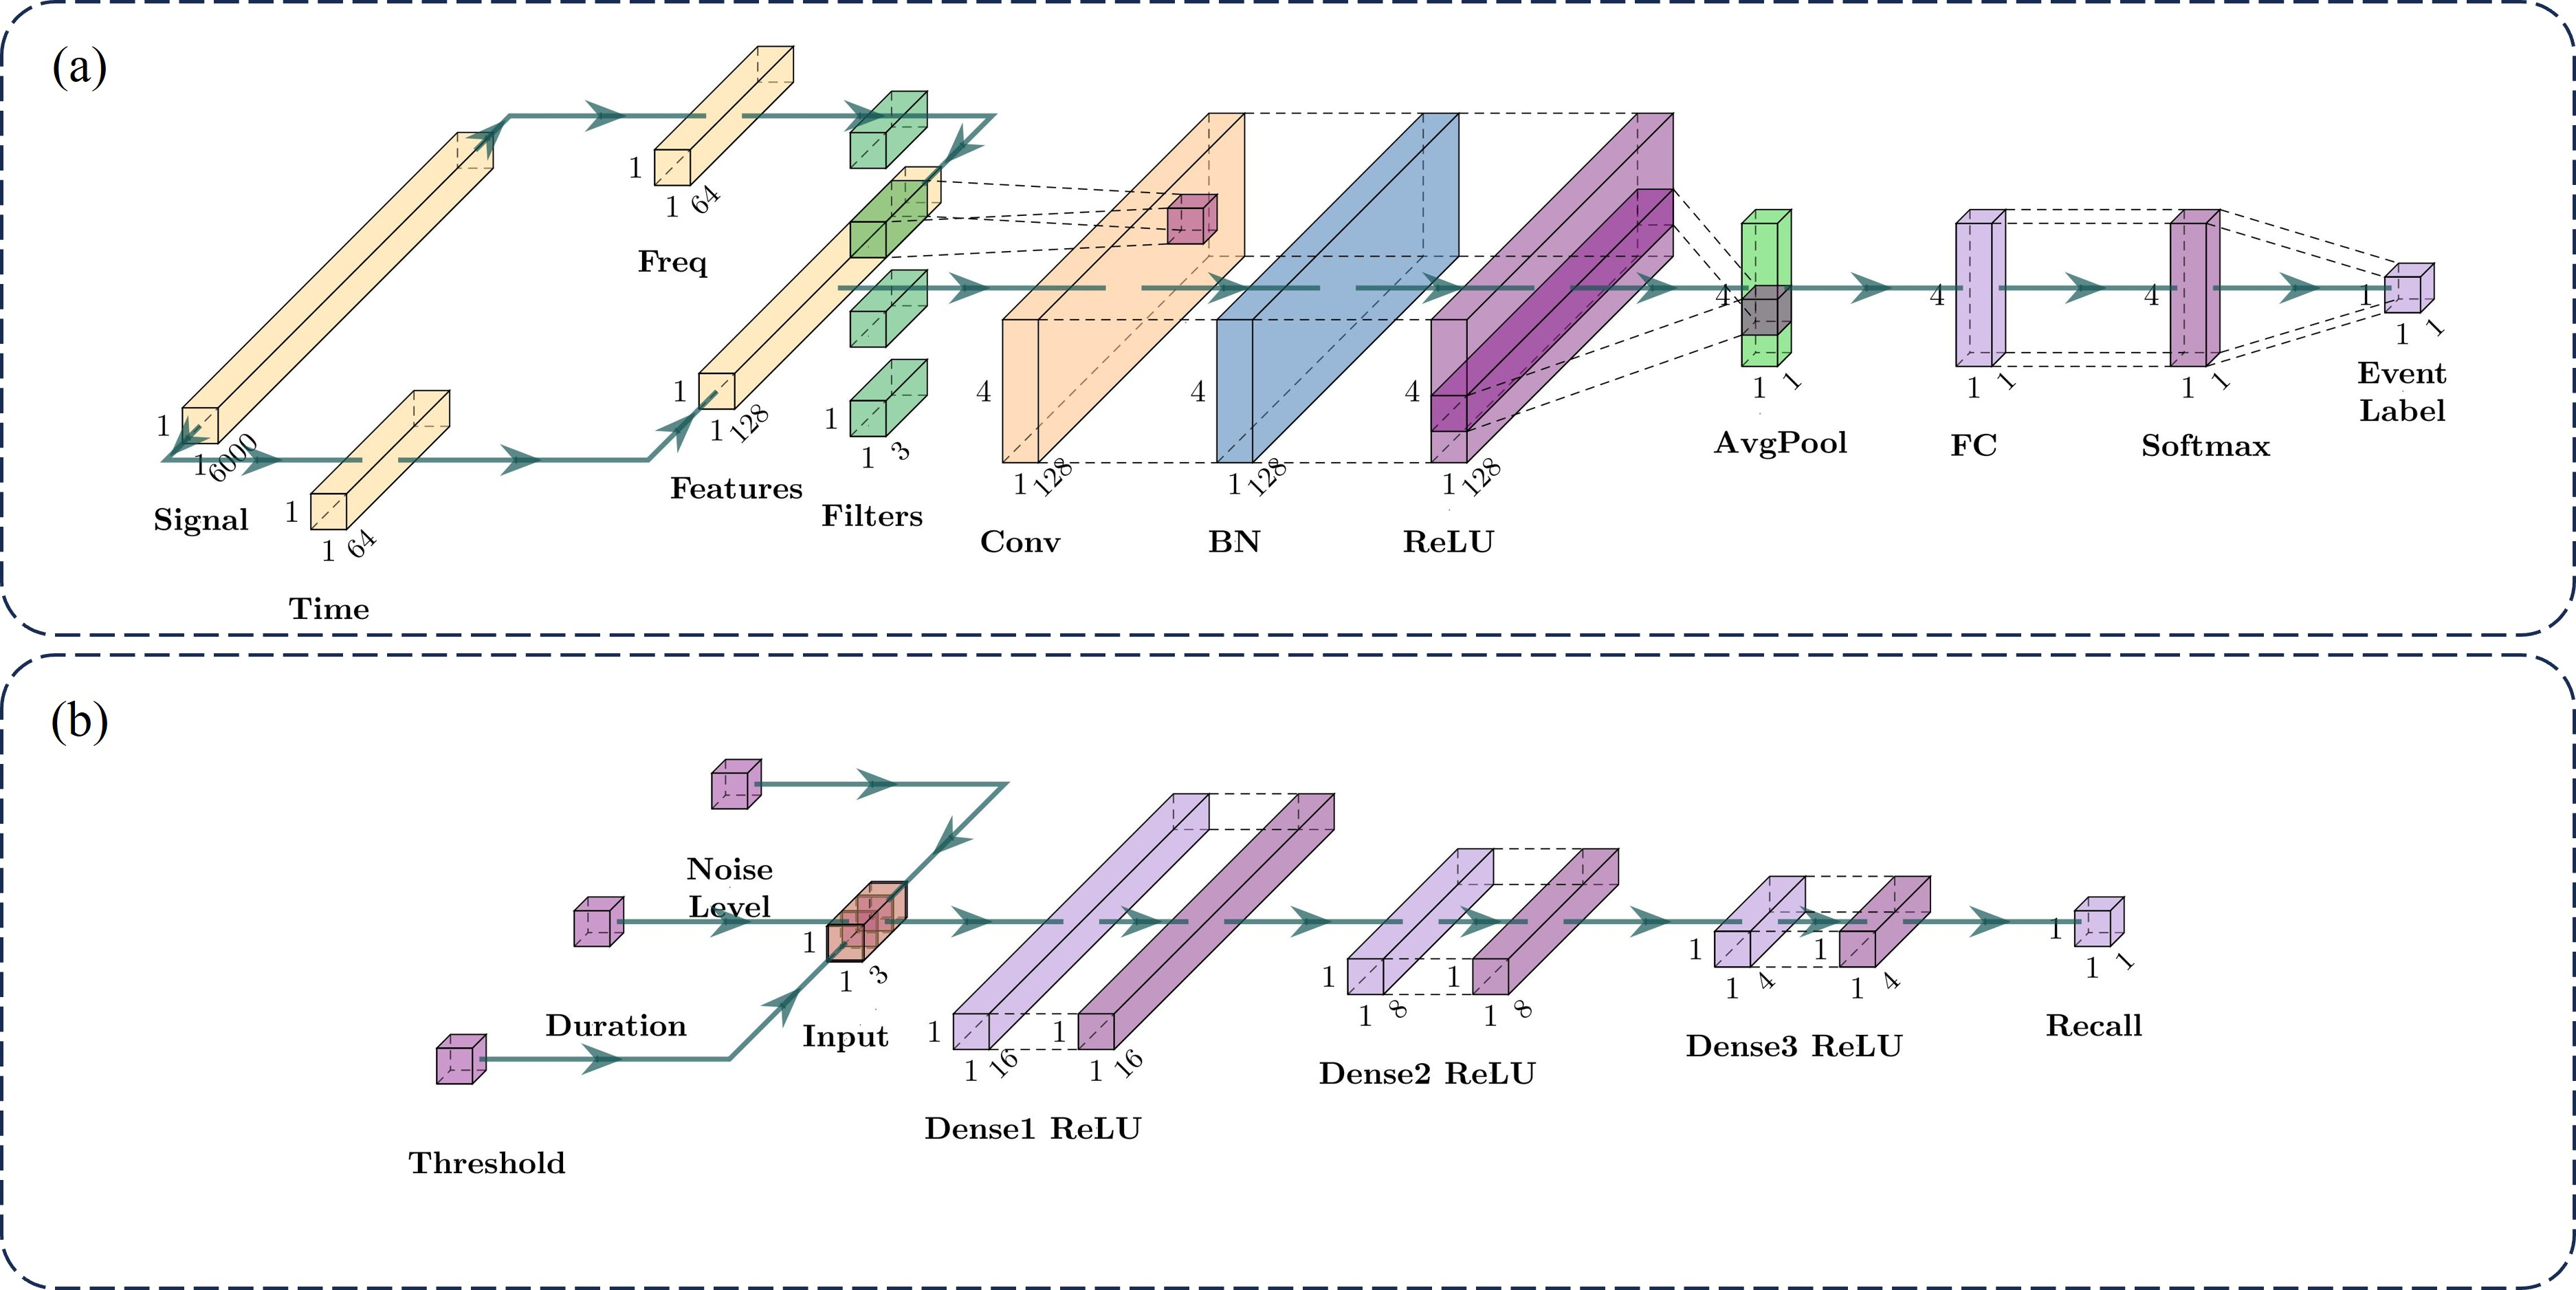
\includegraphics[width=\linewidth]{Fig6.jpg}
    \caption{Neural networks for onboard inference: (a) CNN for event labeling, (b) DNN for recall estimation.}
    \label{fig:Onboard NN}
\end{figure}

\subsubsection{CNN model for onboard event labeling}

In onboard computing, the absence of ground truth labels for collected data complicates determining true positives (TP) and false positives (FP). To address this, a lightweight convolutional neural network (CNN) is designed for deployment on resource-constrained devices. This CNN estimates labels for collected data, enabling TP and FP calculation. The architecture, shown in Figure \ref{fig:Onboard NN} (a), consists of two stages: feature extraction and classification.

The feature extraction stage reduces computational complexity while retaining essential signal characteristics. The raw time-domain signal is downsampled, and its frequency-domain features are derived using the Short-Time Fourier Transform (STFT). Both domains are further downsampled to reduce dimensionality, and their features are concatenated into a unified input vector. This process reduces a 60-second, 100 Hz signal to as few as 128 features, significantly lowering computational load while preserving sufficient information for accurate classification.

The classification stage employs a compact 1D CNN architecture tailored for time-series data. As shown in Figure \ref{fig:Onboard NN} (a), the architecture begins with a 1D convolutional layer featuring four 1-by-3 filters, extracting information from the input features to generate a four-channel output. Batch normalization and ReLU activation are applied, followed by a global average pooling layer, which condenses the information into a single vector. Finally, this vector is passed to a fully connected layer with softmax activation to produce the classification result. This streamlined design harmonizes computational efficiency and classification performance. As revealed by Table \ref{tab:NN}, the CNN classifier model is highly lightweight, with only 142 parameters (572 bytes), making it suitable for onboard deployment.

\begin{table}[h!]
    \centering
    \caption{Neural Network Parameters Summary}
    \label{tab:NN}
    \renewcommand{\arraystretch}{1.5} % vertical spacing
    {\fontfamily{ptm}\selectfont % Times New Roman
    \small
    \begin{tabular}{lll}
        \toprule
        \textbf{Parameter Type}  & \textbf{CNN Classifier} & \textbf{DNN Predictor} \\
        \midrule
        Total Parameters         & 142 (572.00 B) & 209 (836.00 B) \\
        Trainable Parameters     & 44 (176.00 B)  & 209 (836.00 B) \\
        Non-trainable Parameters & 8 (32.00 B)    & 0   (0.00 B)   \\
        Optimizer Parameters     & 90 (364.00 B)  & 0   (0.00 B)   \\
        \bottomrule
    \end{tabular}
    } % Times New Roman
\end{table}

\subsubsection{DNN model for onboard recall estimation}

Unlike precision, which is derived from collected data, recall estimation addresses the partial observability issue due to events that fail to trigger high-resolution sensing. To overcome this, a lightweight deep neural network (DNN) is developed to directly estimate recall, as illustrated in Figure \ref{fig:Onboard NN} (b). The DNN evaluates system performance under specific triggering parameters, with threshold, duration, and noise level selected as inputs. Noise level is critical, as events submerged in noise are harder to detect \citep{han_electrocardiogramsignaldenoising_2017}. The network architecture, optimized through iterative refinements, consists of three fully connected layers with 16, 8, and 4 neurons, each followed by ReLU activation, and a single output neuron predicting recall. This lightweight model has 209 parameters (836 bytes), as detailed in Table \ref{tab:NN}.

System performance depends on both triggering parameters and data distribution. While noise level is included as an input, other factors like event frequency and distribution are harder to quantify. To address this, a digital twin generates artificial data distributions for optimization and evaluation. For training, datasets of events and noise at varying levels are combined, and recall values are calculated for discretized triggering parameters. This yields recall data under diverse conditions, which are used to train the DNN. In real-world applications, the system calculates noise levels from input signals and predicts recall for given triggering parameters. In practice, as more real-world event records are collected over time, artificial data distributions can be gradually replaced, enabling continuous system improvement. Further details on artificial data generation will be discussed in Section \ref{sec:edge_deployment_strategy}.

\subsection{The controller}
\label{component-controller}

In the whole feedback loop, the controller acts as both the brain and the heart, steering the system toward its optimal configuration. Its primary responsibilities are to identify the optimal configuration and determine how to reach it efficiently. In the context of SATM, the controller dynamically adjusts the triggering parameters based on feedback from the estimator, optimizing the $F_{\beta}$ score. This process faces two significant challenges: (1) the system operates as a black-box optimization problem due to its complex nature without explicit mathematical form, and (2) high observation costs arise from extensive data collection and processing required to evaluate the $F_{\beta}$ score, which imposes substantial overhead on resource-constrained edge devices. To address these challenges, the controller employs Bayesian Optimization (BO), a technique well-suited for black-box problems with high observation costs \citep{agrawal_bayesianoptimization_2021}.

\subsubsection{Bayesian Optimization framework}

The goal of BO is to iteratively find the optimal parameters $\boldsymbol{\hat{x}}$ in a predefined search space $\boldsymbol{\mathcal{X}}$ that maximize an objective function $f(\boldsymbol{x})$:

\begin{equation}
\boldsymbol{\hat{x}} = \arg \max_{\boldsymbol{x} \in \boldsymbol{\mathcal{X}}} f(\boldsymbol{x}).
\end{equation}

BO uses a surrogate model $\boldsymbol{\mathcal{M}}$ and an acquisition function $\boldsymbol{\mathcal{S}}$ to iteratively select parameters $\boldsymbol{x}_t$. The acquisition function balances exploration and exploitation to determine the next parameters to evaluate:

\begin{equation}
\boldsymbol{x}_t = \arg \max_{\boldsymbol{x} \in \boldsymbol{\mathcal{X}}} \boldsymbol{\mathcal{S}}(\boldsymbol{x}, \boldsymbol{\mathcal{M}}).
\end{equation}

After evaluating $f(\boldsymbol{x}_t)$, the resulting pair $(\boldsymbol{x}_t, f(\boldsymbol{x}_t))$ is added to the dataset $\boldsymbol{\mathcal{D}}$. This process repeats until a stopping criterion, such as reaching a maximum number of iterations $T$ or a negligible improvement threshold, is met. Algorithm \ref{alg:SMBO} outlines the BO process \citep{agrawal_bayesianoptimization_2021}.

\begin{algorithm}[H]
    \caption{Bayesian Optimization Algorithm Framework}
    \label{alg:SMBO}
    \begin{algorithmic}[1]
        \STATE \textbf{Input:} Search space $\boldsymbol{\mathcal{X}}$, objective function $f$, surrogate model $\boldsymbol{\mathcal{M}}$, acquisition function $\boldsymbol{\mathcal{S}}$
        \STATE \textbf{Output:} Dataset $\boldsymbol{\mathcal{D}}$ (set of sampled points and their evaluations)
        \STATE Initialize dataset: $\boldsymbol{\mathcal{D}} \gets \text{InitSamples}(f, \boldsymbol{\mathcal{X}})$
        \FOR{$i = |\boldsymbol{\mathcal{D}}|$ to $T$}
            \STATE Fit the model: $p(y \mid \boldsymbol{x}, \boldsymbol{\mathcal{D}}) \gets \text{FitModel}(\boldsymbol{\mathcal{M}}, \boldsymbol{\mathcal{D}})$
            \STATE Select next point: $x_i \gets \arg \max_{\boldsymbol{x} \in \boldsymbol{\mathcal{X}}} \boldsymbol{\mathcal{S}}(\boldsymbol{x}, p(y \mid \boldsymbol{x}, \boldsymbol{\mathcal{D}}))$
            \STATE Evaluate objective function: $y_i \gets f(x_i)$
            \STATE Update dataset: $\boldsymbol{\mathcal{D}} \gets \boldsymbol{\mathcal{D}} \cup \{(x_i, y_i)\}$
        \ENDFOR
        \STATE Pick the best point from the dataset $\boldsymbol{\mathcal{D}}$ as the optimum: $\boldsymbol{\hat{x}} \gets \arg \max_{(\boldsymbol{x}, y) \in \boldsymbol{\mathcal{D}}} y$
    \end{algorithmic}
\end{algorithm}

The BO process can be roughly divided into two stages: initialization and iteration. Initialization stage is to generate an initial dataset $\boldsymbol{\mathcal{D}}$ by randomly sampling points from the search space $\boldsymbol{\mathcal{X}}$. The following stage, iteration, is to use the acquisition function $\boldsymbol{\mathcal{S}}$ to determine the next sampling point to observe and to update the surrogate model $\boldsymbol{\mathcal{M}}$. This process continues until the stopping criterion is met, ensuring efficient optimization even under constraints.

Through the whole process of BO, there are some key concepts to be noted:

\begin{itemize}
    \item Search Space $\boldsymbol{\mathcal{X}}$: The search space defines the feasible region where the optimal parameters are sought. Based on prior knowledge and constraints, the search space is confined to save computational resources and time. Note that for SATM, the threshold is continuous, while the duration is discrete (integer values standing for the number of sampling points). The duration can be treated as continuous variable first and then rounded to the nearest meaningful integer.
    \item Objective Function $f$: The objective function maps the triggering parameters to the $F_{\beta}$ score, quantifying the performance of the system under specific configurations. Yet, there is no explicit mathematical form for $f$ in SATM, making it a black-box problem. 
    \item Surrogate Model $\boldsymbol{\mathcal{M}}$ : As the objective function is unknown, the surrogate model is used to approximate it. The surrogate model is updated iteratively based on the dataset $\boldsymbol{\mathcal{D}}$ to predict the objective function at unobserved points \citep{frazier_tutorialbayesianoptimization_2018}. 
    \item Aquisition Function $\boldsymbol{\mathcal{S}}$: The acquisition function guides the selection of the next point to evaluate. It balances exploration and exploitation, aiming to find the optimal parameters efficiently.
    \item Dataset $\boldsymbol{\mathcal{D}}$: The dataset $\boldsymbol{\mathcal{D}}$ stores the sampled points and corresponding evaluations. It is updated iteratively as new points are evaluated, which also records the history of the optimization process. Note that based on the additive nature of the dataset, the optimization can be divided into multiple stages, which is the foundation for the multi-stage deployment strategy proposed in Section \ref{sec:edge_deployment_strategy}.
\end{itemize}

\subsubsection{Surrogate model based on Gaussian Process Regression (GPR)}
In SATM, the surrogate model is constructed using GPR \citep{cui_adaptiveedgeintelligence_2025}. Compared to the unknown latent objective function, the surrogate model features many great mathematical properties, such as differentiability, continuity, and smoothness. These properties make GPR an ideal choice for approximating the objective function in the black-box optimization problem. A Gaussian Process (GP) is defined as a collection of random variables, any finite number of which follow a joint Gaussian distribution \citep{agrawal_bayesianoptimization_2021}. It is typically represented by a mean function $\mu(x)$ and a covariance function $ Cov(x,x') $. A GP $f(x)$, including noise, can be expressed as:

\begin{equation}
\label{eq:gaussian-process-noise}
    f(x) \sim \mathcal{GP}(\mu(x), Cov(x, x') + \sigma_n^2 \delta_{xx'})
\end{equation}

where \( \sigma_n^2 \) represents the noise variance, and \( \delta_{xx'} \) is the Kronecker delta function. The mean and covariance functions are defined as $\mu(x) = \mathbb{E}(f(x))$ and $Cov(x, x') = \mathbb{E}((f(x) - \mu(x))(f(x') - \mu(x')))$, respectively.

With noisy observation vector $\boldsymbol{y}$, the joint distribution between the observed values $\boldsymbol{y}$ and the predicted values $\boldsymbol{f^*}$ follows a joint Gaussian distribution:

\begin{equation}
\label{eq:joint-gaussian-noise}
    \begin{bmatrix} \boldsymbol{y} \\ \boldsymbol{f^*} \end{bmatrix} \sim \mathcal{N} \left( \begin{bmatrix} \mu(\boldsymbol{x}) \\ \mu(\boldsymbol{x^*}) \end{bmatrix}, \begin{bmatrix} Cov(\boldsymbol{x}, \boldsymbol{x}) + \sigma_n^2 \mathbf{I}, & Cov(\boldsymbol{x}, \boldsymbol{x^*}) \\ Cov(\boldsymbol{x^*}, \boldsymbol{x}), & Cov(\boldsymbol{x^*}, \boldsymbol{x^*}) \end{bmatrix} \right)
\end{equation}

where $ Cov(\boldsymbol{x}, \boldsymbol{x}) $ is the covariance matrix of the observed point vector, $ Cov(\boldsymbol{x}, \boldsymbol{x^*}) $ is the covariance between the observed point vector $ \boldsymbol{x} $ and the prediction point vector $ \boldsymbol{x^*} $, and $ \sigma_n^2 $ accounts for the noise.

Given this joint distribution, the conditional distribution of the prediction vector $ \boldsymbol{f^*} $ can be derived as:

\begin{equation}
\label{eq:conditional-gaussian-noise}
    \boldsymbol{f^*} | \boldsymbol{y} \sim \mathcal{GP}(\mu(\boldsymbol{x^*}), \sigma^2(\boldsymbol{x^*}))
\end{equation}

with

\begin{equation}
\label{eq:mean-prediction-noise}
    \mu(\boldsymbol{x^*}) = Cov(\boldsymbol{x^*}, \boldsymbol{x}) \left( Cov(\boldsymbol{x}, \boldsymbol{x}) + \sigma_n^2 \mathbf{I} \right)^{-1} \boldsymbol{y}
\end{equation}

\begin{equation}
\label{eq:variance-prediction-noise}
    \sigma^2(\boldsymbol{x^*}) = Cov(\boldsymbol{x^*}, \boldsymbol{x^*}) - Cov(\boldsymbol{x^*}, \boldsymbol{x}) \left( Cov(\boldsymbol{x}, \boldsymbol{x}) + \sigma_n^2 \mathbf{I} \right)^{-1} Cov(\boldsymbol{x},\boldsymbol{x^*})
\end{equation}

These equations enable predictions while accounting for noisy observations, with the noise variance \( \sigma_n^2 \) incorporated into the covariance matrix.

In this research, the Matern 2.5 kernel is chosen as the kernel function for covariance computation due to its flexibility in modeling both smooth and rough functions. The Matern 2.5 kernel is defined as:

\begin{equation}
\label{eq:matern-2.5-kernel}
k(\boldsymbol{x}, \boldsymbol{x'}) = \alpha \left( 1 + \frac{\sqrt{5} d}{\lambda} + \frac{5 d^2}{3 \lambda^2} \right) \exp\left(-\frac{\sqrt{5} d}{\lambda}\right)
\end{equation}

where $ d = \|\boldsymbol{x} - \boldsymbol{x'}\| $ is the Euclidean distance between $ \boldsymbol{x} $ and $ \boldsymbol{x'} $, $ \alpha $ is the scaling factor, and $ \lambda $ is the length scale parameter.

As shown above, the Gaussian process model involves three key hyperparameters: the scaling factor $ \alpha $, the length scale $ \lambda $, and the noise variance $ \sigma_n^2 $. To optimize these hyperparameters, the marginal likelihood of the Gaussian process is maximized, which can be expressed as:

\begin{equation}
\label{eq:marginal-likelihood}
    Pr(\boldsymbol{y}|\boldsymbol{x}, \boldsymbol{\theta}) = \text{Norm}_{\boldsymbol{y}}(\mu, Cov(\boldsymbol{x}, \boldsymbol{x}) + \sigma_n^2 \mathbf{I})
\end{equation}

where $ \boldsymbol{\theta} = (\alpha, \lambda, \sigma_n^2) $ represents the hyperparameters, $ \boldsymbol{y} $ is the observed data, $ \boldsymbol{x} $ is the input data, $ \mu $ is the mean function, and $ Cov(\boldsymbol{x}, \boldsymbol{x}) $ is the covariance matrix.

Maximizing the marginal likelihood helps to find the set of hyperparameters that best fit the data while balancing model complexity. Even if the hyperparameters are not perfectly optimized, the Gaussian process can still provide a reasonable approximation of the objective function. A simple and effective approach to hyperparameter optimization is grid search, which can identify a good set of hyperparameters.

\subsubsection{Acquisition function based on Upper Confidence Bound (UCB)}

In BO, the acquisition function plays a critical role in determining the next observation point for evaluation. These functions guide the trade-off between exploration (sampling in areas of high uncertainty) and exploitation (sampling in areas expected to yield high values based on prior observations). In SATM, the UCB acquisition function \citep{agrawal_bayesianoptimization_2021} is chosen for its effectiveness and ease for implementation. It combines the mean prediction $ \mu(x^*) $ and the uncertainty estimate $ \sigma(x^*) $, and is defined as:

\begin{equation}
    UCB(x^*) = \mu(x^*) + \beta^{1/2} \sigma(x^*)
\end{equation}

where $ \mu(x^*) $ represents the predicted mean (exploitation), $ \sigma(x^*) $ represents the predicted uncertainty (exploration), and $ \beta^{1/2} $ is a tunable parameter that controls the balance between exploration and exploitation. UCB considers both the predicted value and uncertainty to select the next observation point, thereby effectively exploring areas of uncertainty while refining regions with higher predicted values. As shown in Algorithm \ref{alg:SMBO}, by maximizing the acquisition function, herein UCB, the next observation point is determined, and the optimization process continues iteratively. In SATM, Monte Carlo method is used to maximize the acquisition function, which is easy and efficient for edge deployment.

\section{Edge deployment strategy} 
\label{sec:edge_deployment_strategy}

The primary objective of SATM is to facilitate onboard adaptive fine-tuning of trigger parameters to optimize the $F_{\beta}$ score. Given the resource constraints inherent in edge devices, the deployment strategy must prioritize computational efficiency and lightweight implementation without compromising reliability or accuracy. The overarching philosophy is to leverage the digital twin to offload computationally intensive tasks, thereby reducing the computational burden during the actual deployment phase. This approach ensures a high-performance starting point for lightweight online fine-tuning. The strategy comprises two critical phases: (1) utilizing the digital twin to pre-train a surrogate model and optimize trigger parameters, and (2) deploying the pre-optimized model and parameters to edge devices for onboard fine-tuning, enabling real-time adaptive adjustments with minimal computational overhead. Section \ref{sec:smart_adaptive_triggering_mechanism} introduces the building blocks of SATM from a spatial perspective, while this section focuses on the temporal perspective, outlining the deployment pipeline in chronological order.

\subsection{Stage I: Pre-deployment optimization}

The first stage focuses on pre-deployment optimization using the digital twin to establish a foundation for onboard fine-tuning. The digital twin provides a virtual environment for optimizing the surrogate model, training neural networks, and generating artificial signals for real-time adjustments during deployment. This stage ensures that the system is well-prepared for efficient onboard fine-tuning. 

\subsubsection{Digital twin and pre-optimization}
\label{sec:digital_twin_pre-optimization}

The construction of the digital twin can be considered from two perspectives: spatial and temporal. From the spatial perspective, all building blocks of SATM, as detailed in Section \ref{sec:smart_adaptive_triggering_mechanism}, must be properly established before integration into a unified framework. This section emphasizes the temporal perspective, focusing on how the digital twin simulates or enhances real-world scenarios in a time-sequenced manner, such as controlling the frequency distribution of events or generating rare events that are difficult to observe in the real world. It is important to note that the key point of the digital twin here is to accelerate optimization and provide functionalities that may not be feasible in real-world deployments, rather than to replicate them exactly.

As discussed in Section \ref{sec:gaps_challenges}, the uncertainty in event distribution poses significant challenges, which can be addressed through digital twin technology by generating artificial event distributions and providing sufficient data for rare events to support optimization and neural network training. To facilitate virtual optimization, we propose a straightforward method for constructing artificial event distributions: for a total of $n$ events in each SATM performance evaluation, half $n/2$ are designated as events of no interest, while the remaining half $n/2$ represent events of interest. If there are $m$ types of events of interest, each type is allocated $n/2m$ events, as illustrated in Figure \ref{fig:Artificial Event Distribution}. The event can be characterized by maximum signal amplitude, and the distribution of the maximum signal amplitude can follow a certain distribution, such as uniform or Gaussian. Compared to real-world cases, the artificial event distribution is more controllable and can be adjusted to cover a wide range of scenarios, especially for rare events that are difficult to observe in practice. If possible, the data distribution can be corrected based on real-world observations. 

One critical issue that requires special attention is ensuring the range of signal amplitudes in the artificial distribution aligns with real-world data, particularly for events of no interest, which in this study are primarily represented by ambient vibrations. This alignment is crucial because a major source of misclassification arises when events of interest are obscured by background noise. Consequently, accurately representing noise levels is paramount in the optimization process and must be carefully addressed to ensure the reliability and effectiveness of the digital twin in simulating real-world conditions.
To some extent, the noise level determines whether the results from the digital twin can be effectively transferred to real-world applications. In short, for pre-optimization, the noise level should align well with real-world data, while the events of interest can be more flexible to cover a wide range of scenarios.

\begin{figure}[htbp]
    \centering
    
\includegraphics[width=\linewidth]{Fig7.jpg}
    \caption{Schematic illustration of artificial event distribution generation.}
    \label{fig:Artificial Event Distribution}
\end{figure}

Compared to the real-world cases, the virtual environment can generate much more events for pre-deployment optimization, enabling the surrogate model to be trained on a more comprehensive dataset and achieve better performance. Since the pre-optimization is conducted in a controlled and resource-rich environment, the computation can be more intensive, so that the surrogate model can be well-trained to provide a high-quality starting point for the onboard fine-tuning. Actually, it is quite likely that the optimal configuration found in the digital twin can also be optimal in the real-world cases, which is the ultimate goal of the pre-deployment optimization. 

\begin{figure}[htbp]
    \centering
    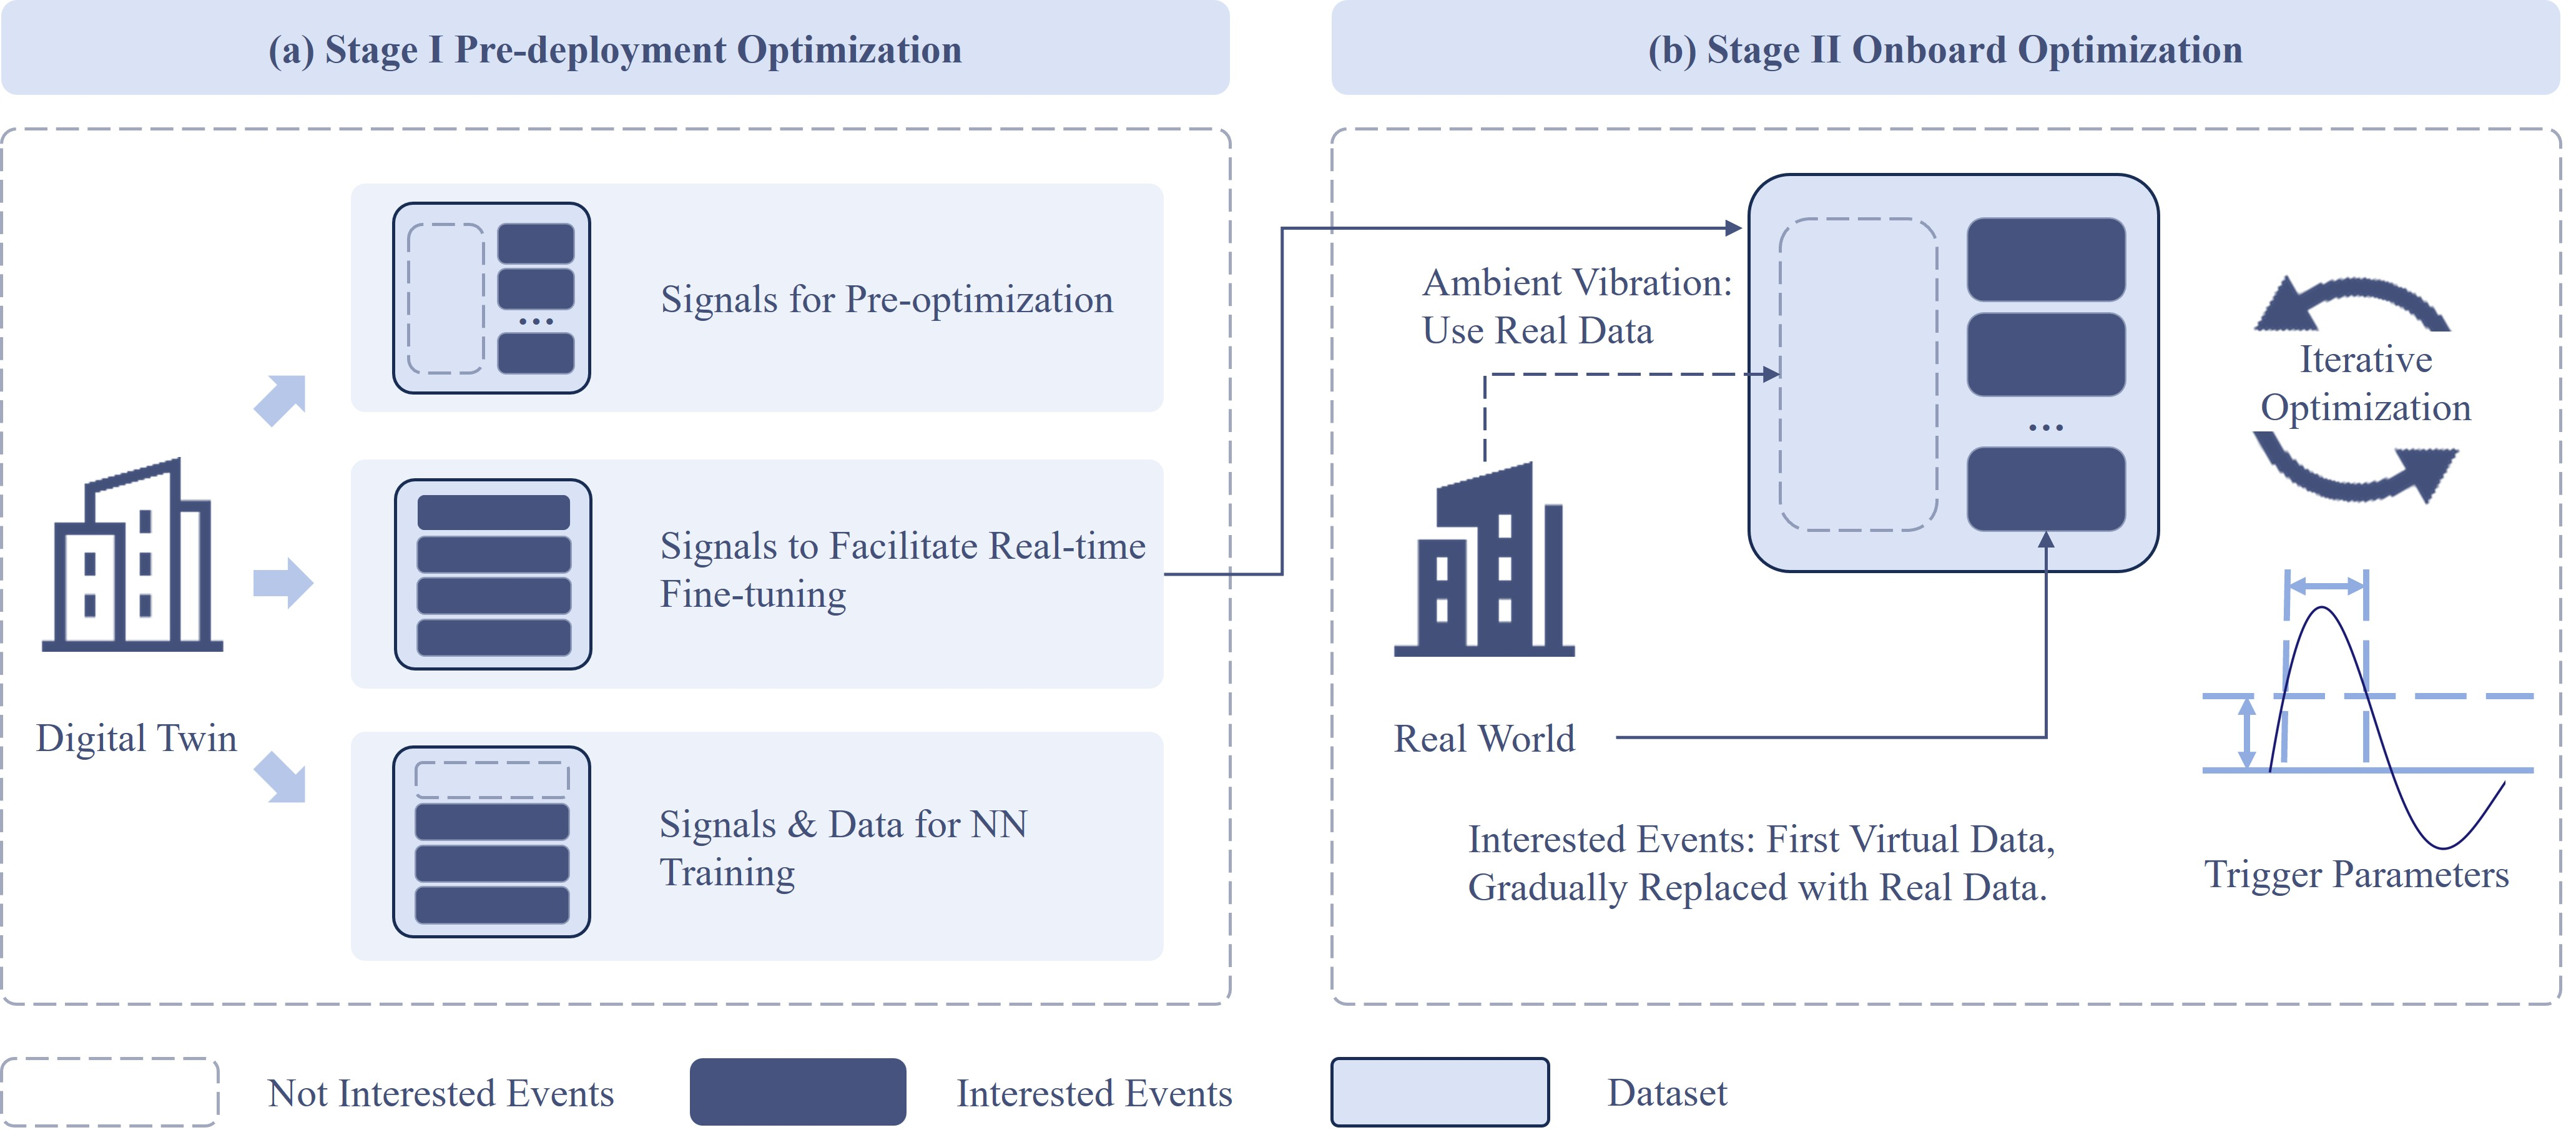
\includegraphics[width=\linewidth]{Fig8.jpg}
    \caption{Schematic illustration of the edge deployment strategy: (a) Stage I: pre-deployment optimization, (b) Stage II: onboard optimization}
    \label{fig:Edge Deployment Strategy}
\end{figure}

\subsubsection{Artificial datasets and neural networks training}
\label{sec:artificial_dataset_nn_training}

Building upon the digital twin framework introduced in Section \ref{sec:digital_twin_pre-optimization}, this section focuses on leveraging the digital twin to generate datasets to facilitate real-world fine-tuning and neural network training for onboard inference. The digital twin enables the characterization of SATM performance based on artificial event distributions, ensuring consistency between simulated and real-world scenarios. It is important to maintain similar event distributions across both environments to ensure the applicability of results from virtual environment to real-world deployments. However, unlike the digital twin, real-world optimization typically operates on smaller datasets, as its primary objective is parameter fine-tuning rather than coarse surrogate model training. Given the ease of capturing ambient vibrations in real-world settings, the artificial datasets for real-world fine-tuning should concentrate exclusively on events of interest.

As outlined in Section \ref{component-estimator}, the system employs two neural networks: a CNN for event labeling and a DNN for recall estimation. The training of these networks is conducted in this stage using data generated by the digital twin. For CNN training, the digital twin generates a sufficient number of diverse event types to ensure robust model training. DNN training, however, presents a more complex scenario, as its input comprises not raw signals but triggering parameters, noise levels, and recall values. To construct the DNN training dataset, the process involves generating events of interest, mixing them with ambient vibration data at varying noise levels, and calculating recall values across different triggering parameters. This dataset is then used to train the DNN for recall estimation. Importantly, the event distribution for DNN training must align with the artificial event distribution established in the digital twin framework to maintain consistency and ensure reliable performance in real-world applications. 

\subsection{Stage II: onboard optimization}

In SHM practice, most wireless sensing devices are micro-controller unit (MCU) level devices, featuring limited computational resources, memory, and power supply. To support the deployment of the proposed SATM, the sensor should have a large volume storage media like SD card. Preferably, the MCU vendor should have a good support for onboard signal processing and AI, for example, STM32Cube-AI from STMicroelectronics, ESP-DSP \citep{espressif_espdsp_2025} and ESP-DL \citep{espressif_espdl_2025} from Espressif. Otherwise, the user should have the ability to port the AI model to the MCU \citep{lee_dualcorebased_2024, lin_mcunettinydeep_2020}. Most importantly, the SATM should be incorporated into the sensor working pipeline, from sensing, data processing, to performance evaluation.

As elaborated in Section \ref{sec:artificial_dataset_nn_training}, for onboard optimization, considering the uncertain real world event distribution and consistency with the surrogate model in stage I, the artificial event distribution and associated datasets are adopted. Note that, the ambient vibration, i.e., the noise part can use real world data as they can be easily captured and matter a lot for event detection.

In nature, the performance evaluation for onboard optimization is based on the synthesized dataset following artificial event distribution which is consistent with the digital twin. To make it more realistic and reliable, the datasets can be gradually replaced with real world data. As mentioned, the noise data can first be replaced with real world data all at once, and then the event data can be gradually replaced as more real world data is collected. This is a continuous improvement process, which can be conducted as a side quest without interrupting the main quest for parameter fine-tuning.

\section{Deployment and validation}
\label{sec:deployment_validation}

\subsection{Experimental setup}

\begin{figure}[htbp]
    \centering
    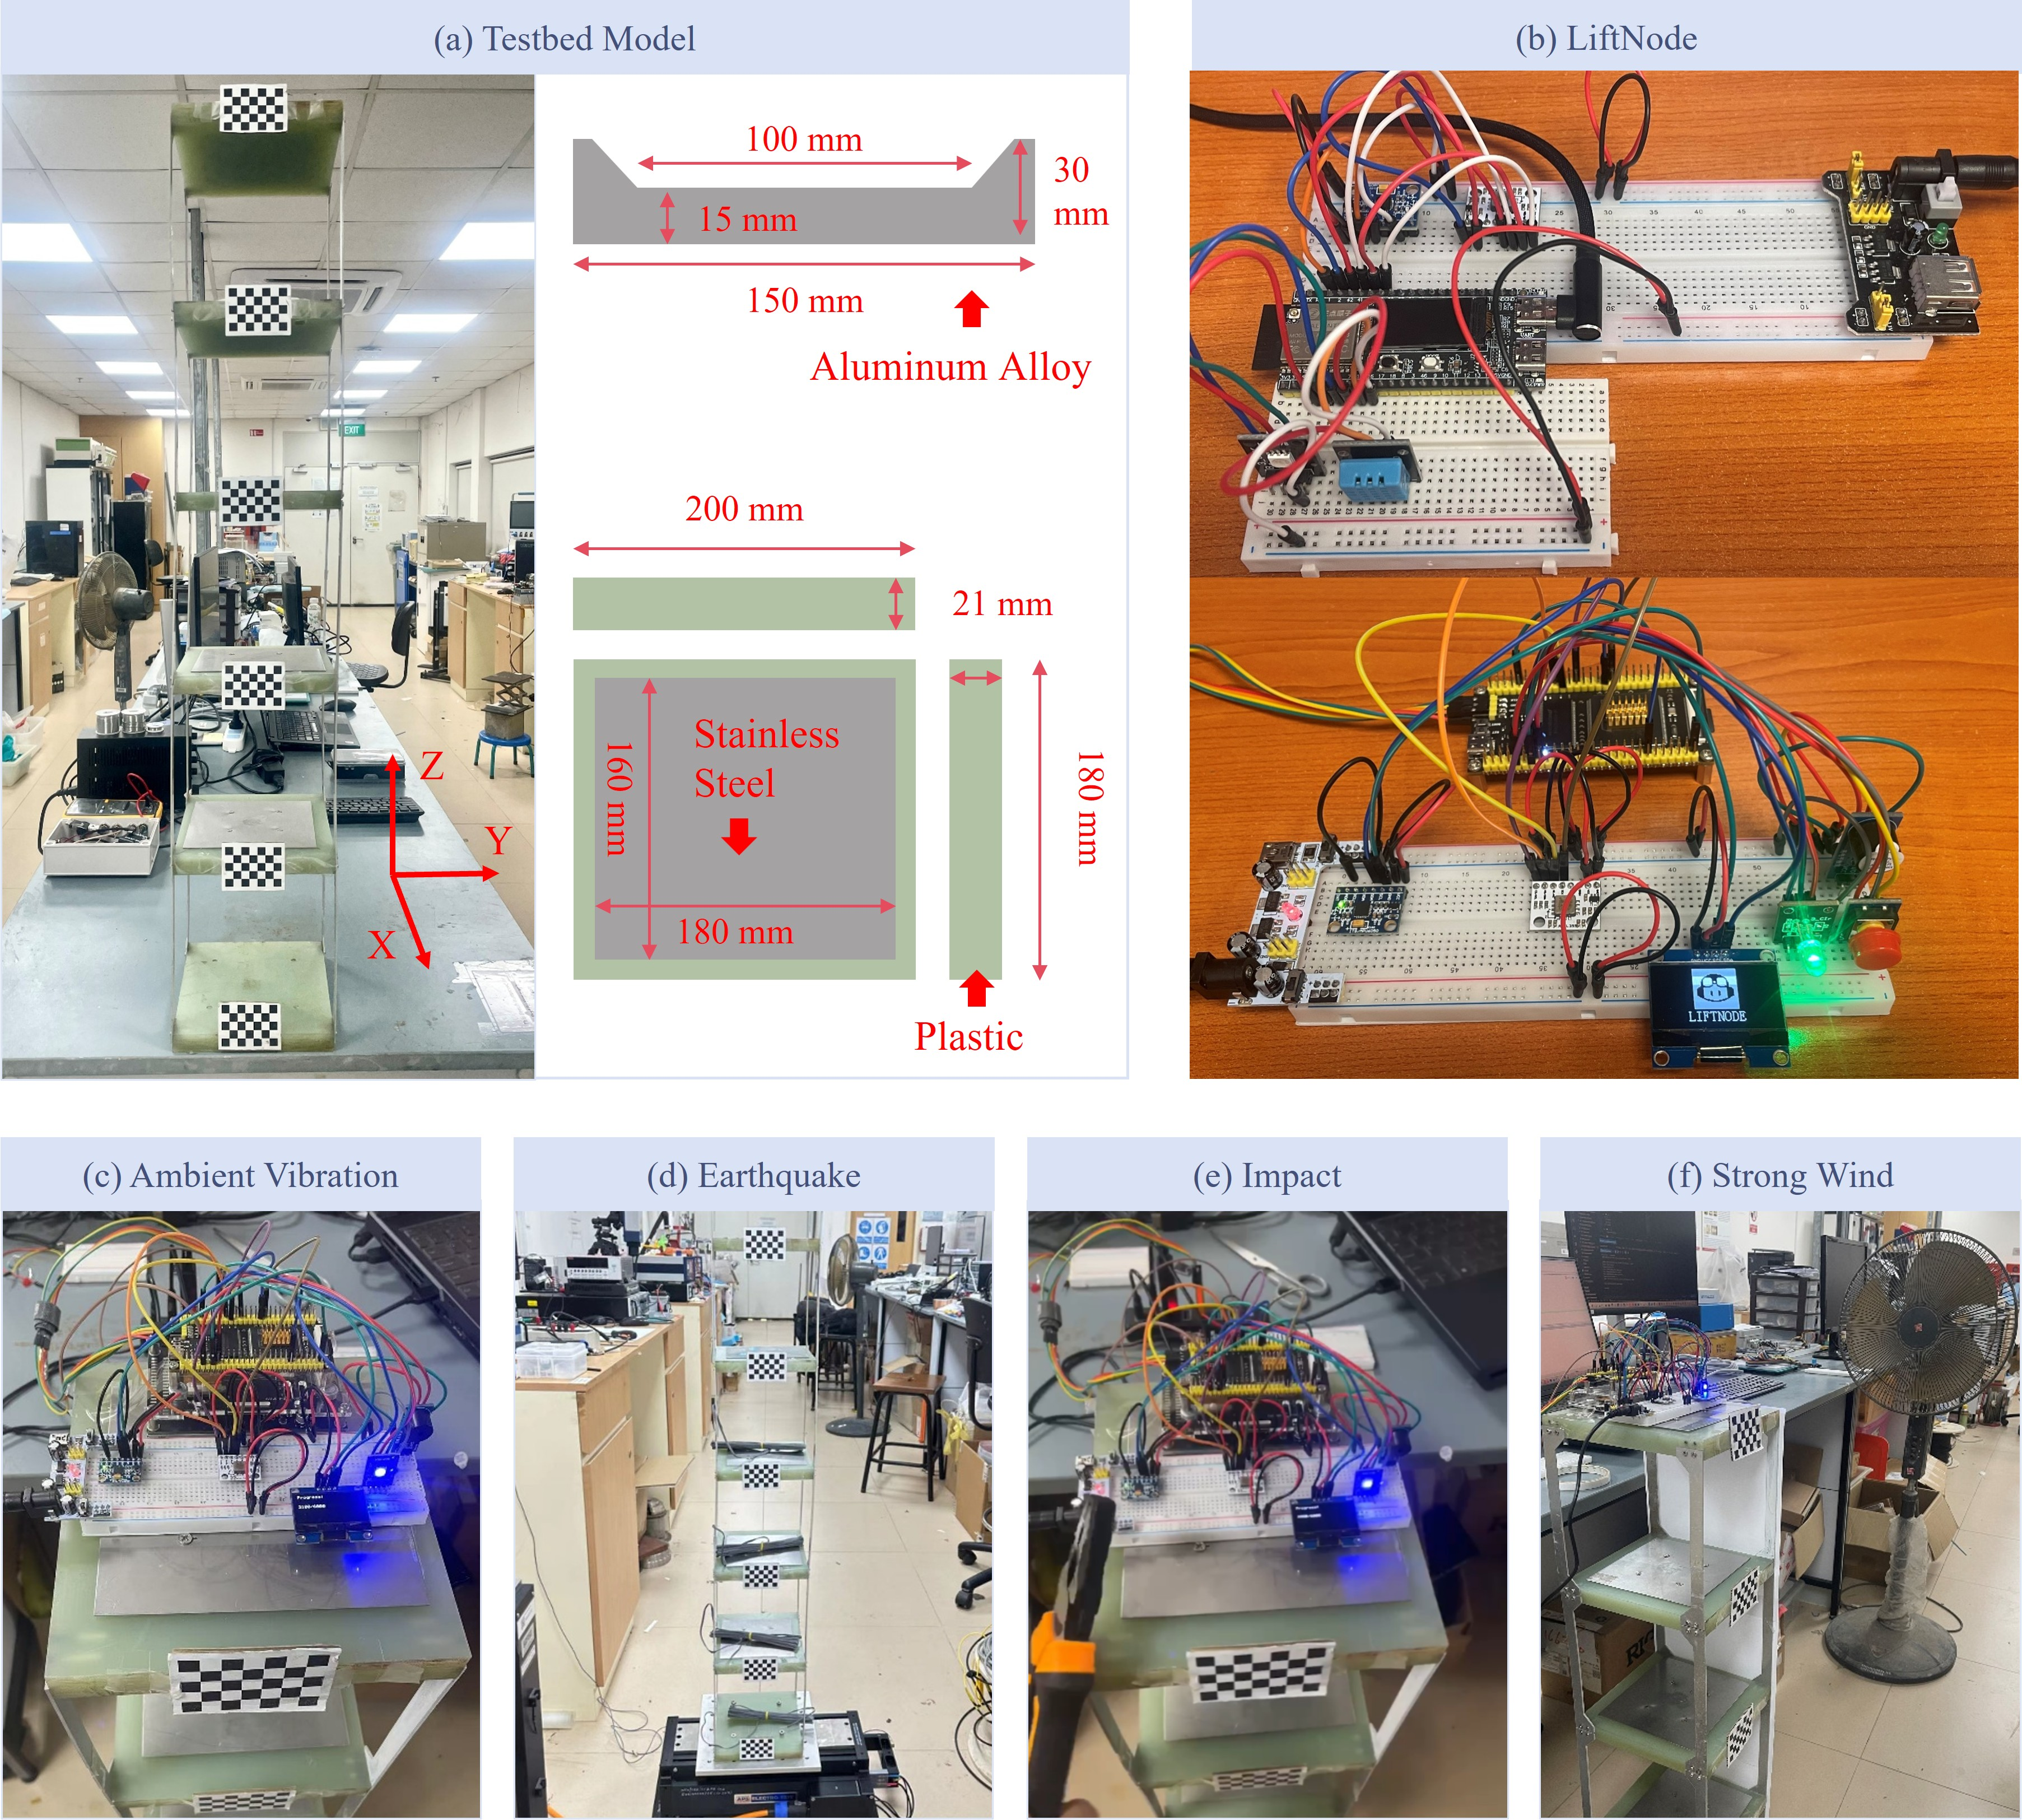
\includegraphics[width=\linewidth]{Fig9.jpg}
    \caption{Experimental setup: (a) testbed model, (b) LiftNode, (c) ambient vibration sensing, (d) earthquake sensing, (e) impact sensing, (f) strong wind sensing.}
    \label{fig:Experimental Setup}
\end{figure}

As illustrated in Figure \ref{fig:Experimental Setup}, a 5-storey structural model serves as the testbed for monitoring and evaluation, and among the 3 axes, Y-axis is selected for evaluation as it features the most significant response. This study utilizes LiftNode, a low-power, cost-effective, and high-performance IoT sensing platform actively developed by the Laboratory of Intelligent Infrastructure (LIFT) at Nanyang Technological University (NTU), for data collection and edge intelligence. To ensure cross-platform compatibility, LiftNode is prototyped with two different main control boards: one based on STM32 and the other on ESP32. In this study, validation is conducted using the ESP32-based LiftNode, which features a dual-core 32-bit MCU running at 480 MHz, 8 MB of RAM, and 16 MB of flash memory. During validation, LiftNode is positioned atop the testbed model, as shown in subplot (c).

Various types of events are examined in this study, each generated using different methods. For ambient vibration sensing, no additional equipment or intervention is required (subplot (c)). Earthquake simulations are performed using a shaker (subplot (d)), impact events are induced with a hammer (subplot (e)), and strong wind conditions are replicated using a fan (subplot (f)). More technical details for validation can be found in Table \ref{tab:optimization-configuration}.

\subsection{Deployment procedures}

\begin{figure}[htbp]
    \centering
    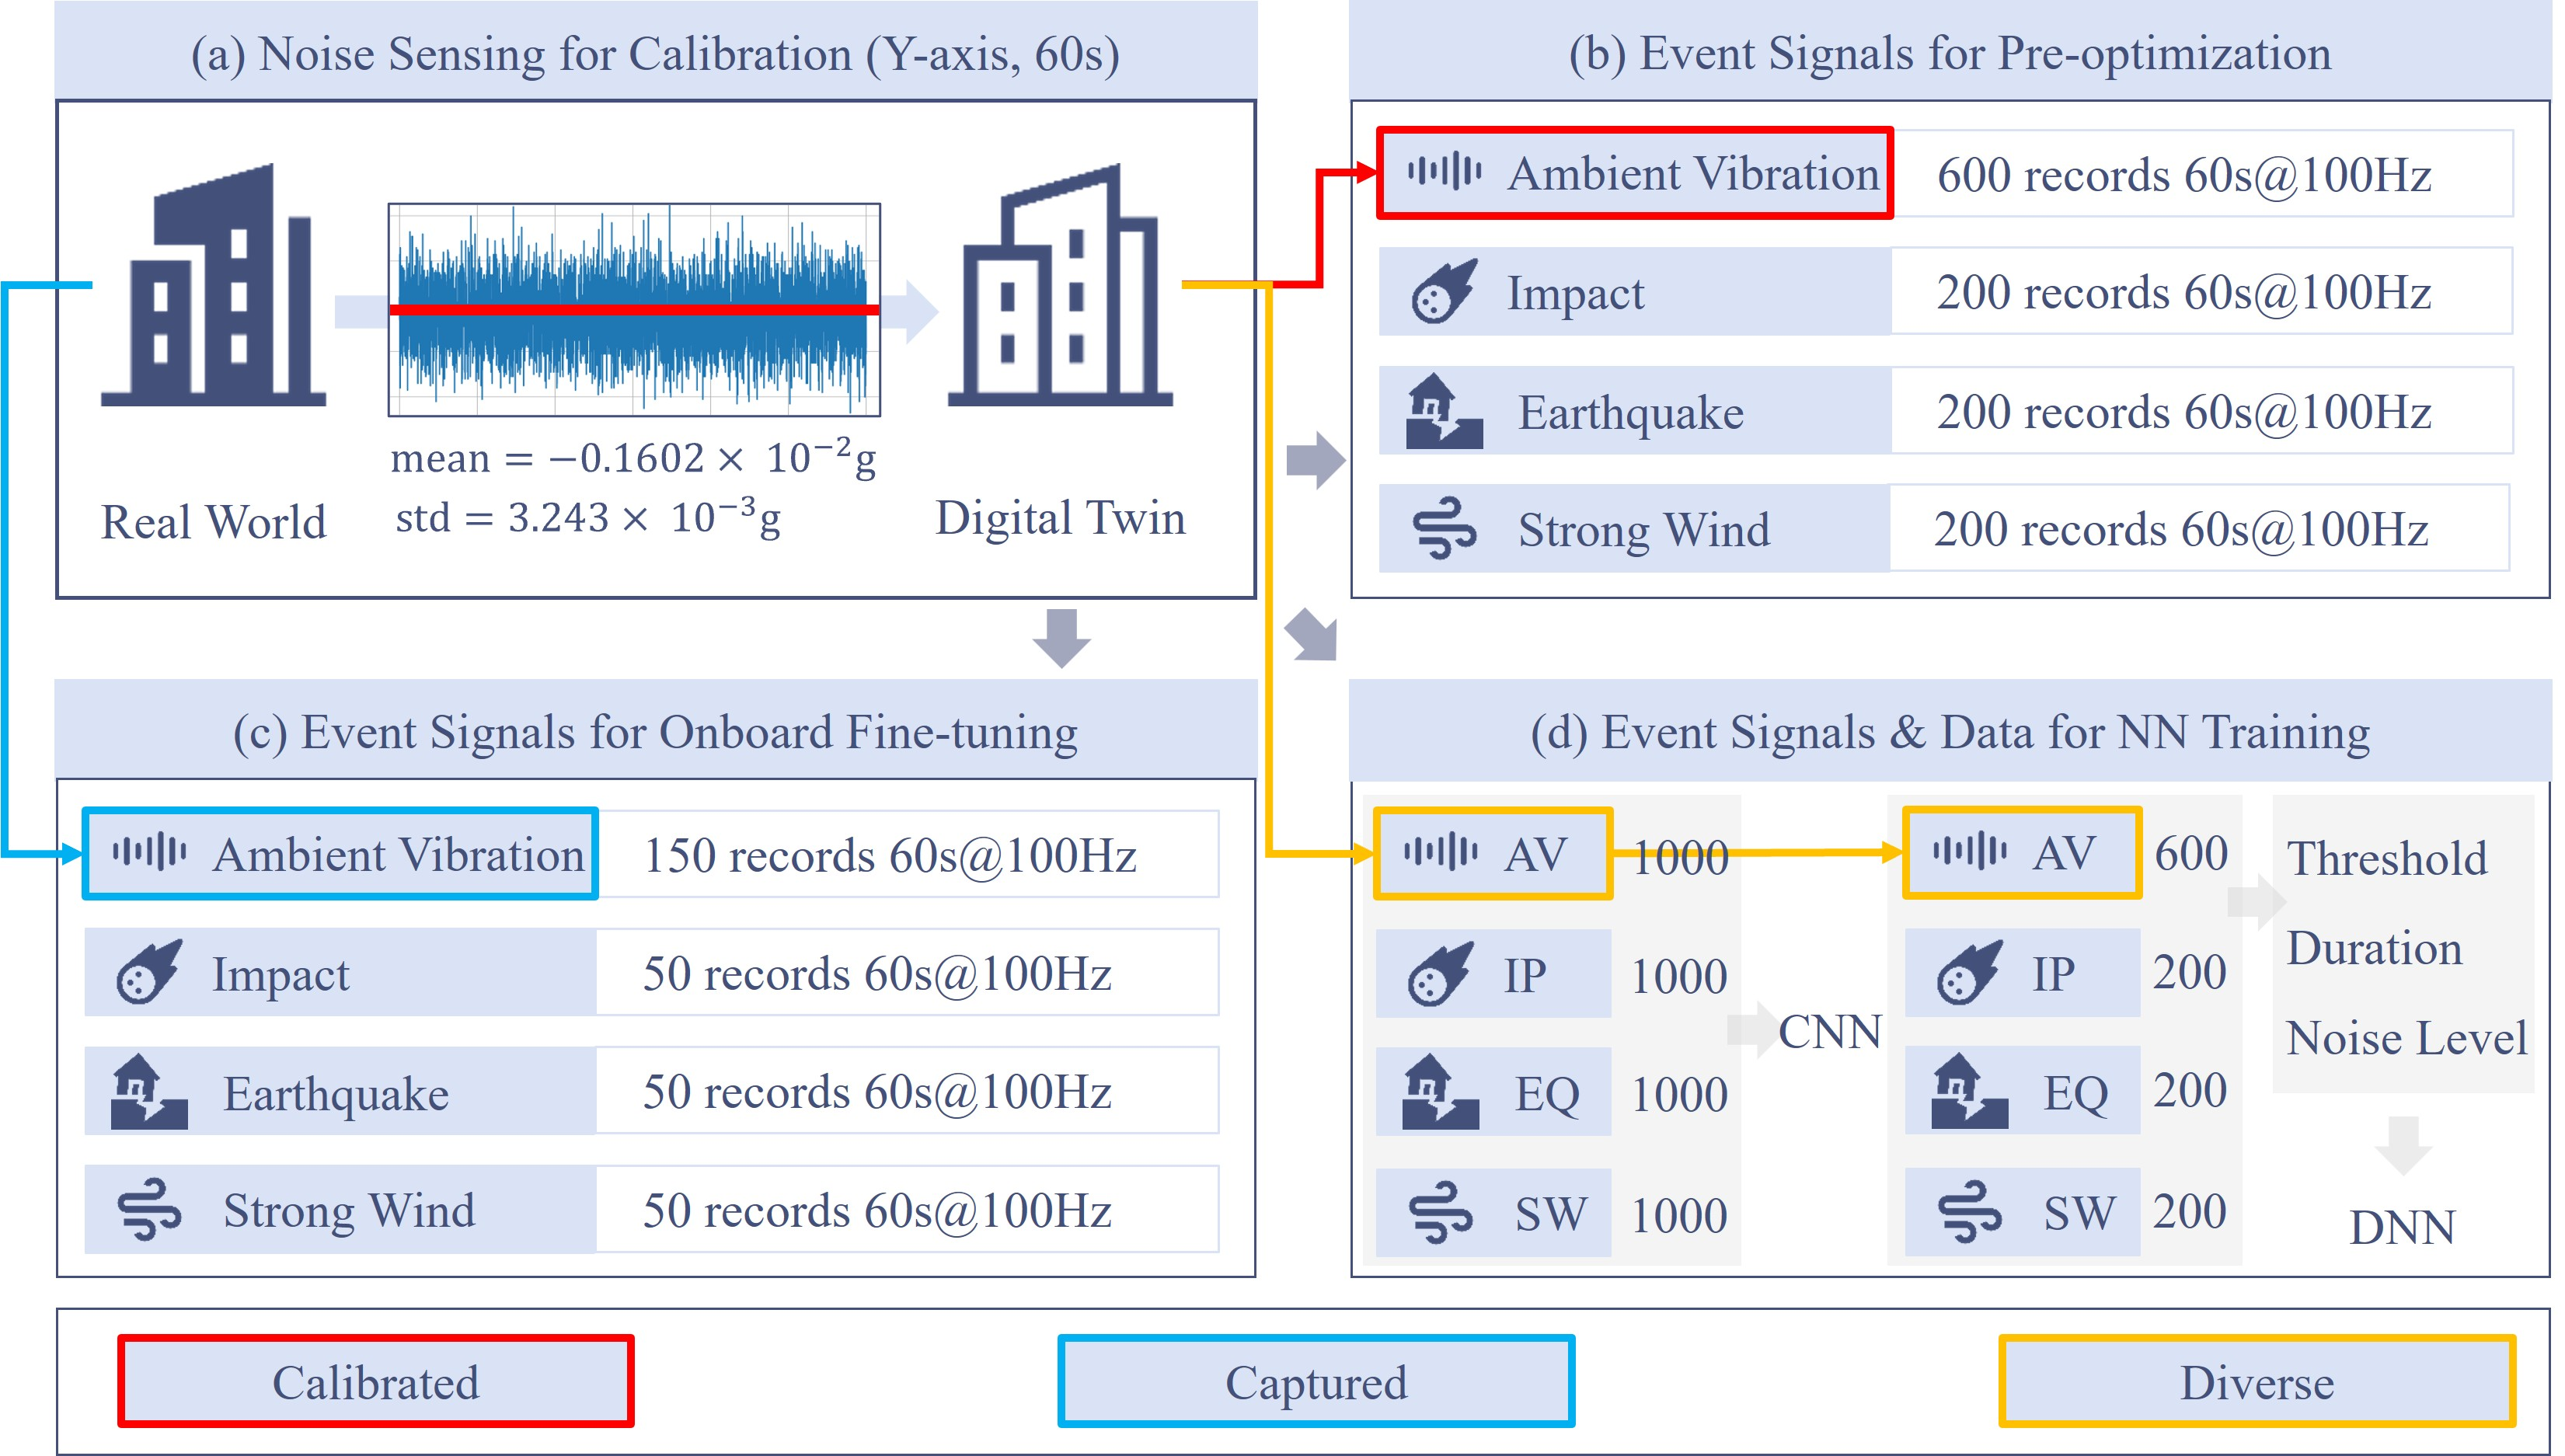
\includegraphics[width=0.9\linewidth]{Fig10.jpg}
    \caption{Signal synthesizing: (a) noise level calibration, (b) generation for pre-optimization, (c) generation for onboard optimization, (d) neural network training.}
    \label{fig:Signal Synthesizing}
\end{figure}

\begin{figure}[htbp]
    \centering
    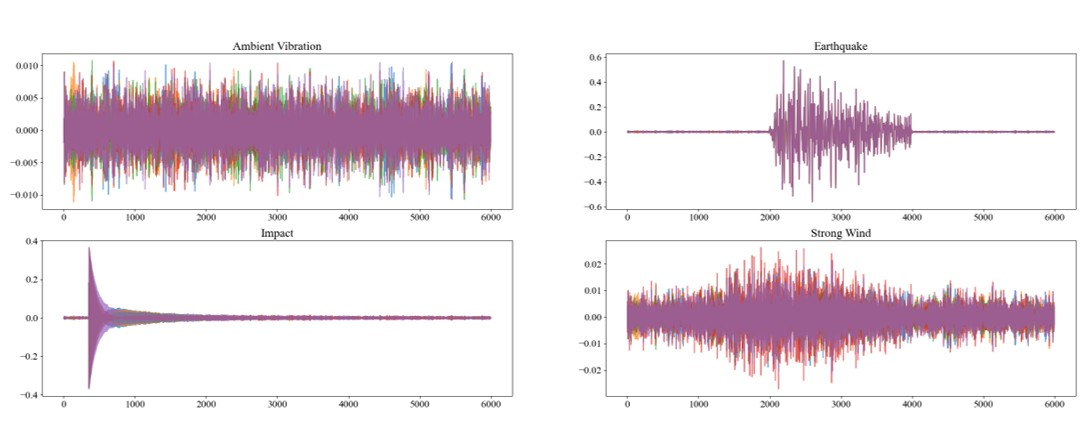
\includegraphics[width=1\linewidth]{Fig11.jpg}
    \caption{Examples of synthesized data.}
    \label{fig: Synthesized Data Example}
\end{figure}

\begin{figure}[htbp]
    \centering
    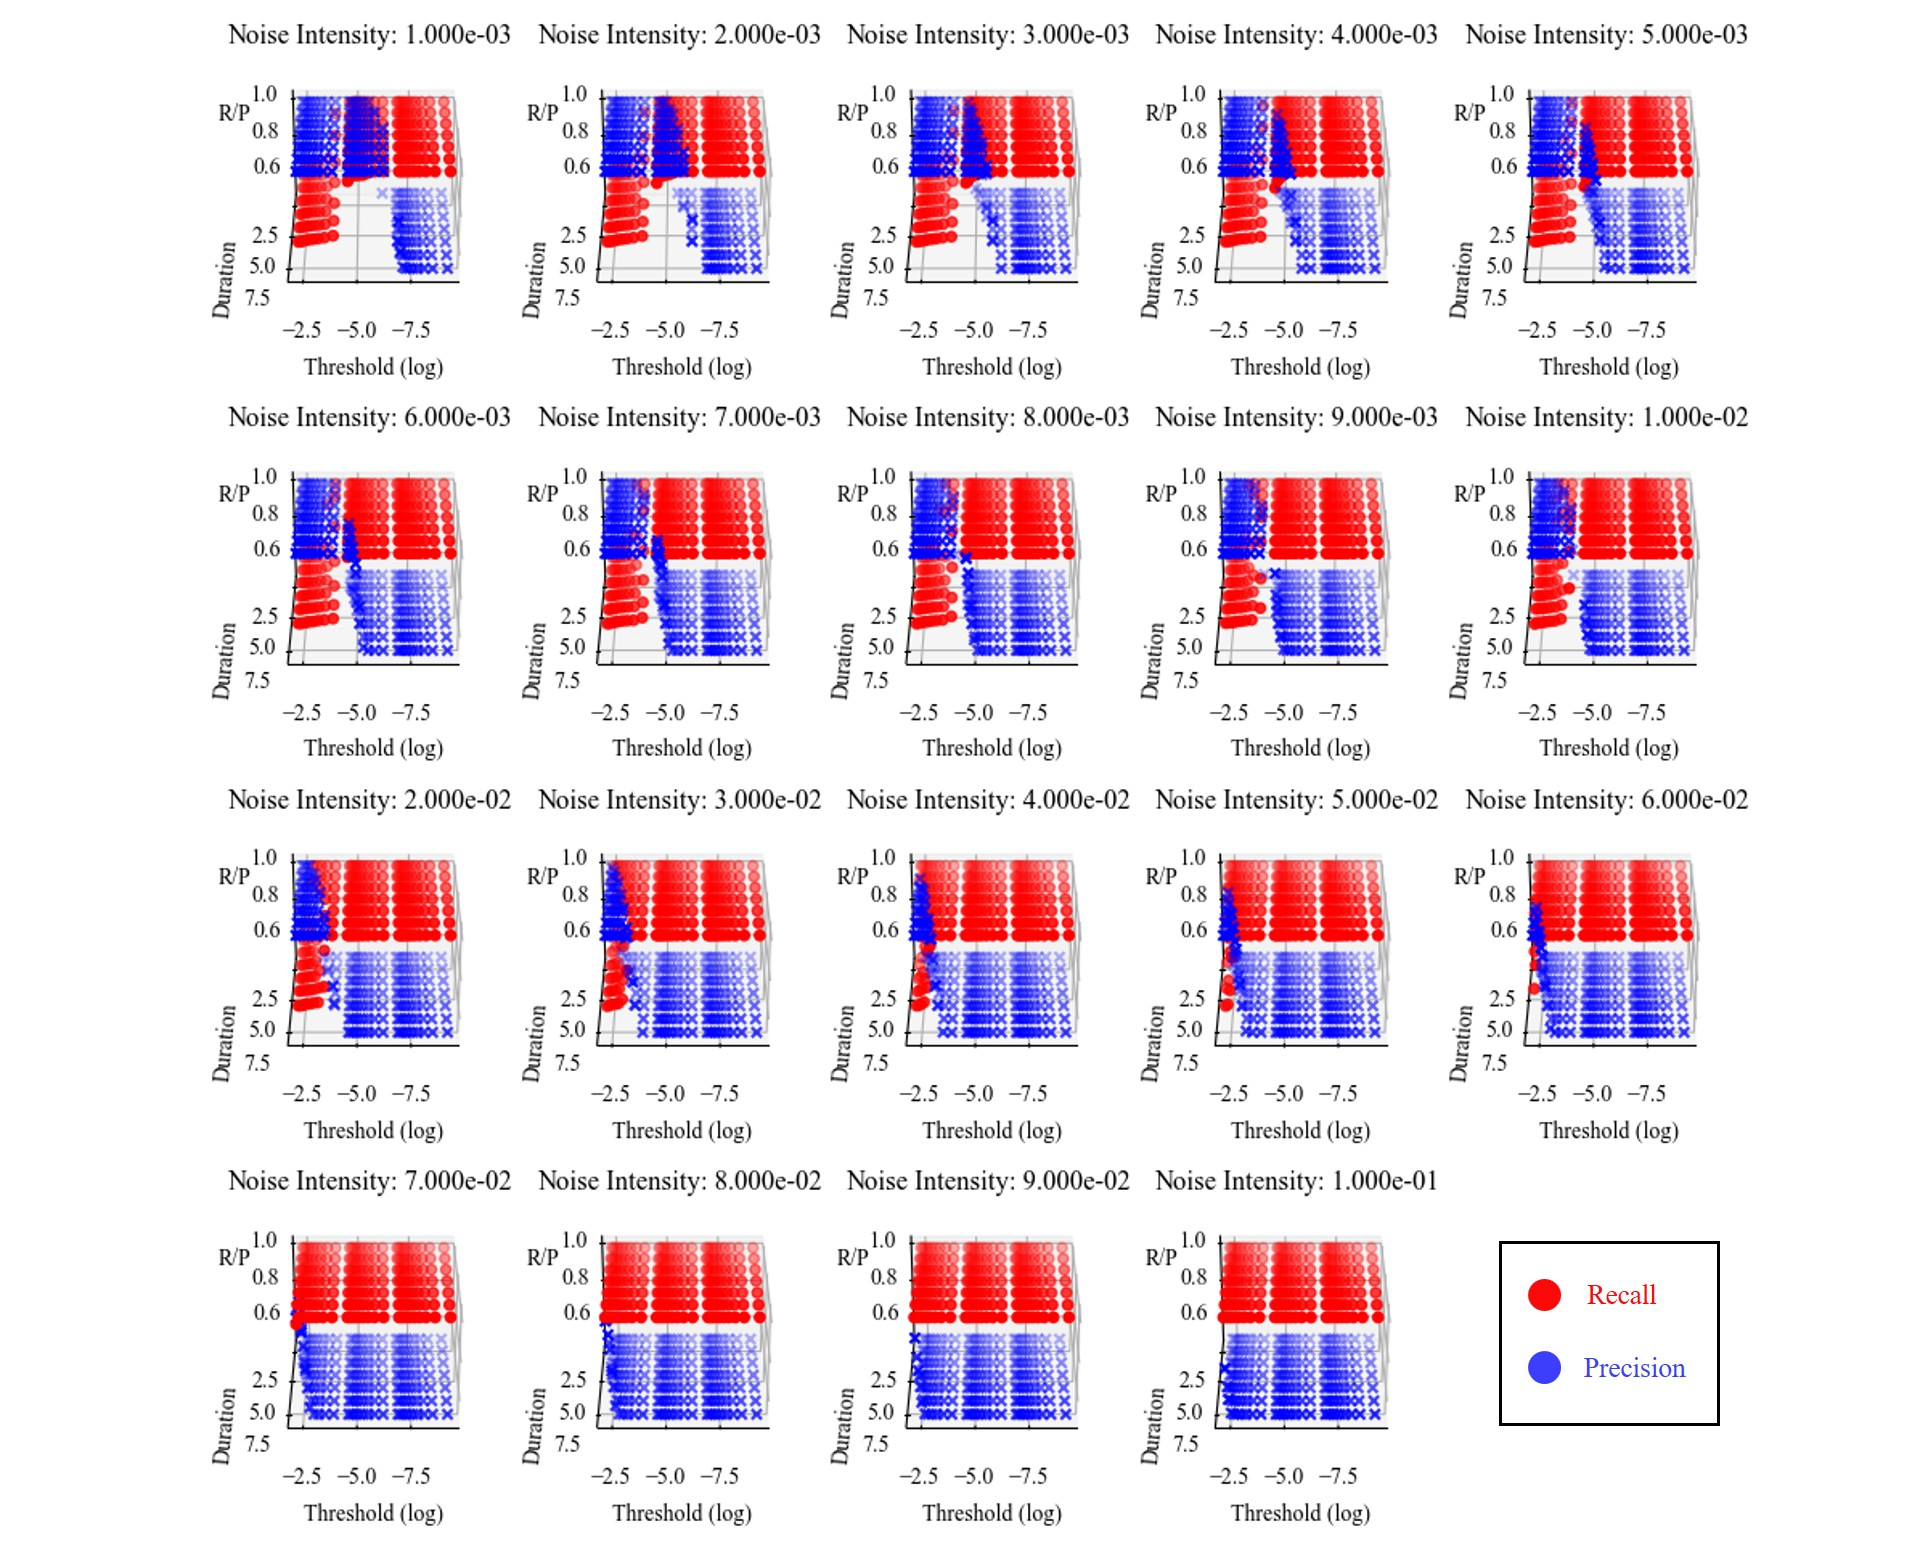
\includegraphics[width=\linewidth]{Fig12.jpg}
    \caption{Dataset for DNN training: recall and precision distributions across the search space under different noise levels.}
    \label{fig: DNN Training Dataset}
\end{figure}

\begin{figure}[htbp]
    \centering
    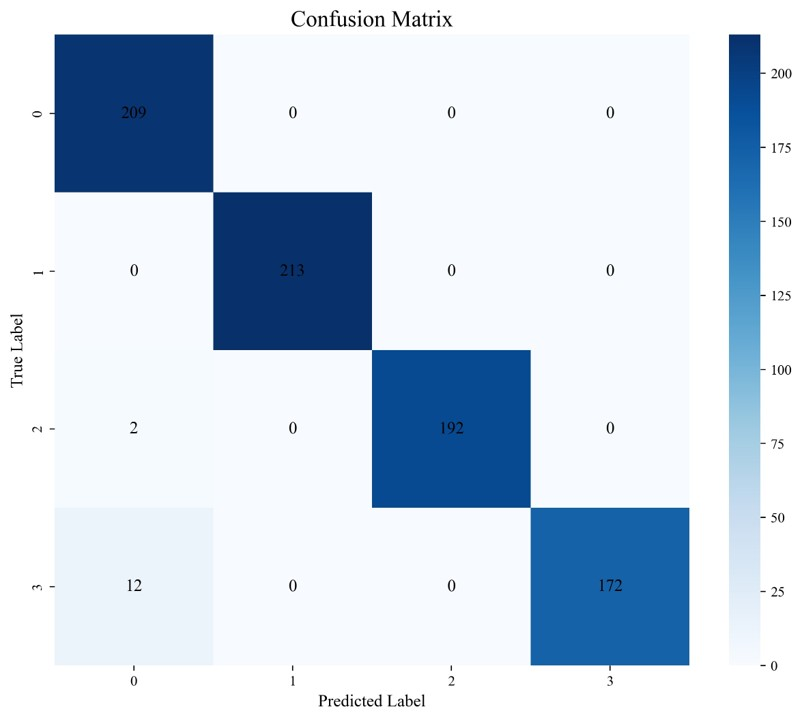
\includegraphics[width=0.35\linewidth]{Fig13.jpg}
    \caption{CNN confusion matrix.}
    \label{fig: CNN Confusion Matrix}
\end{figure}

\begin{figure}[htbp]
    \centering
    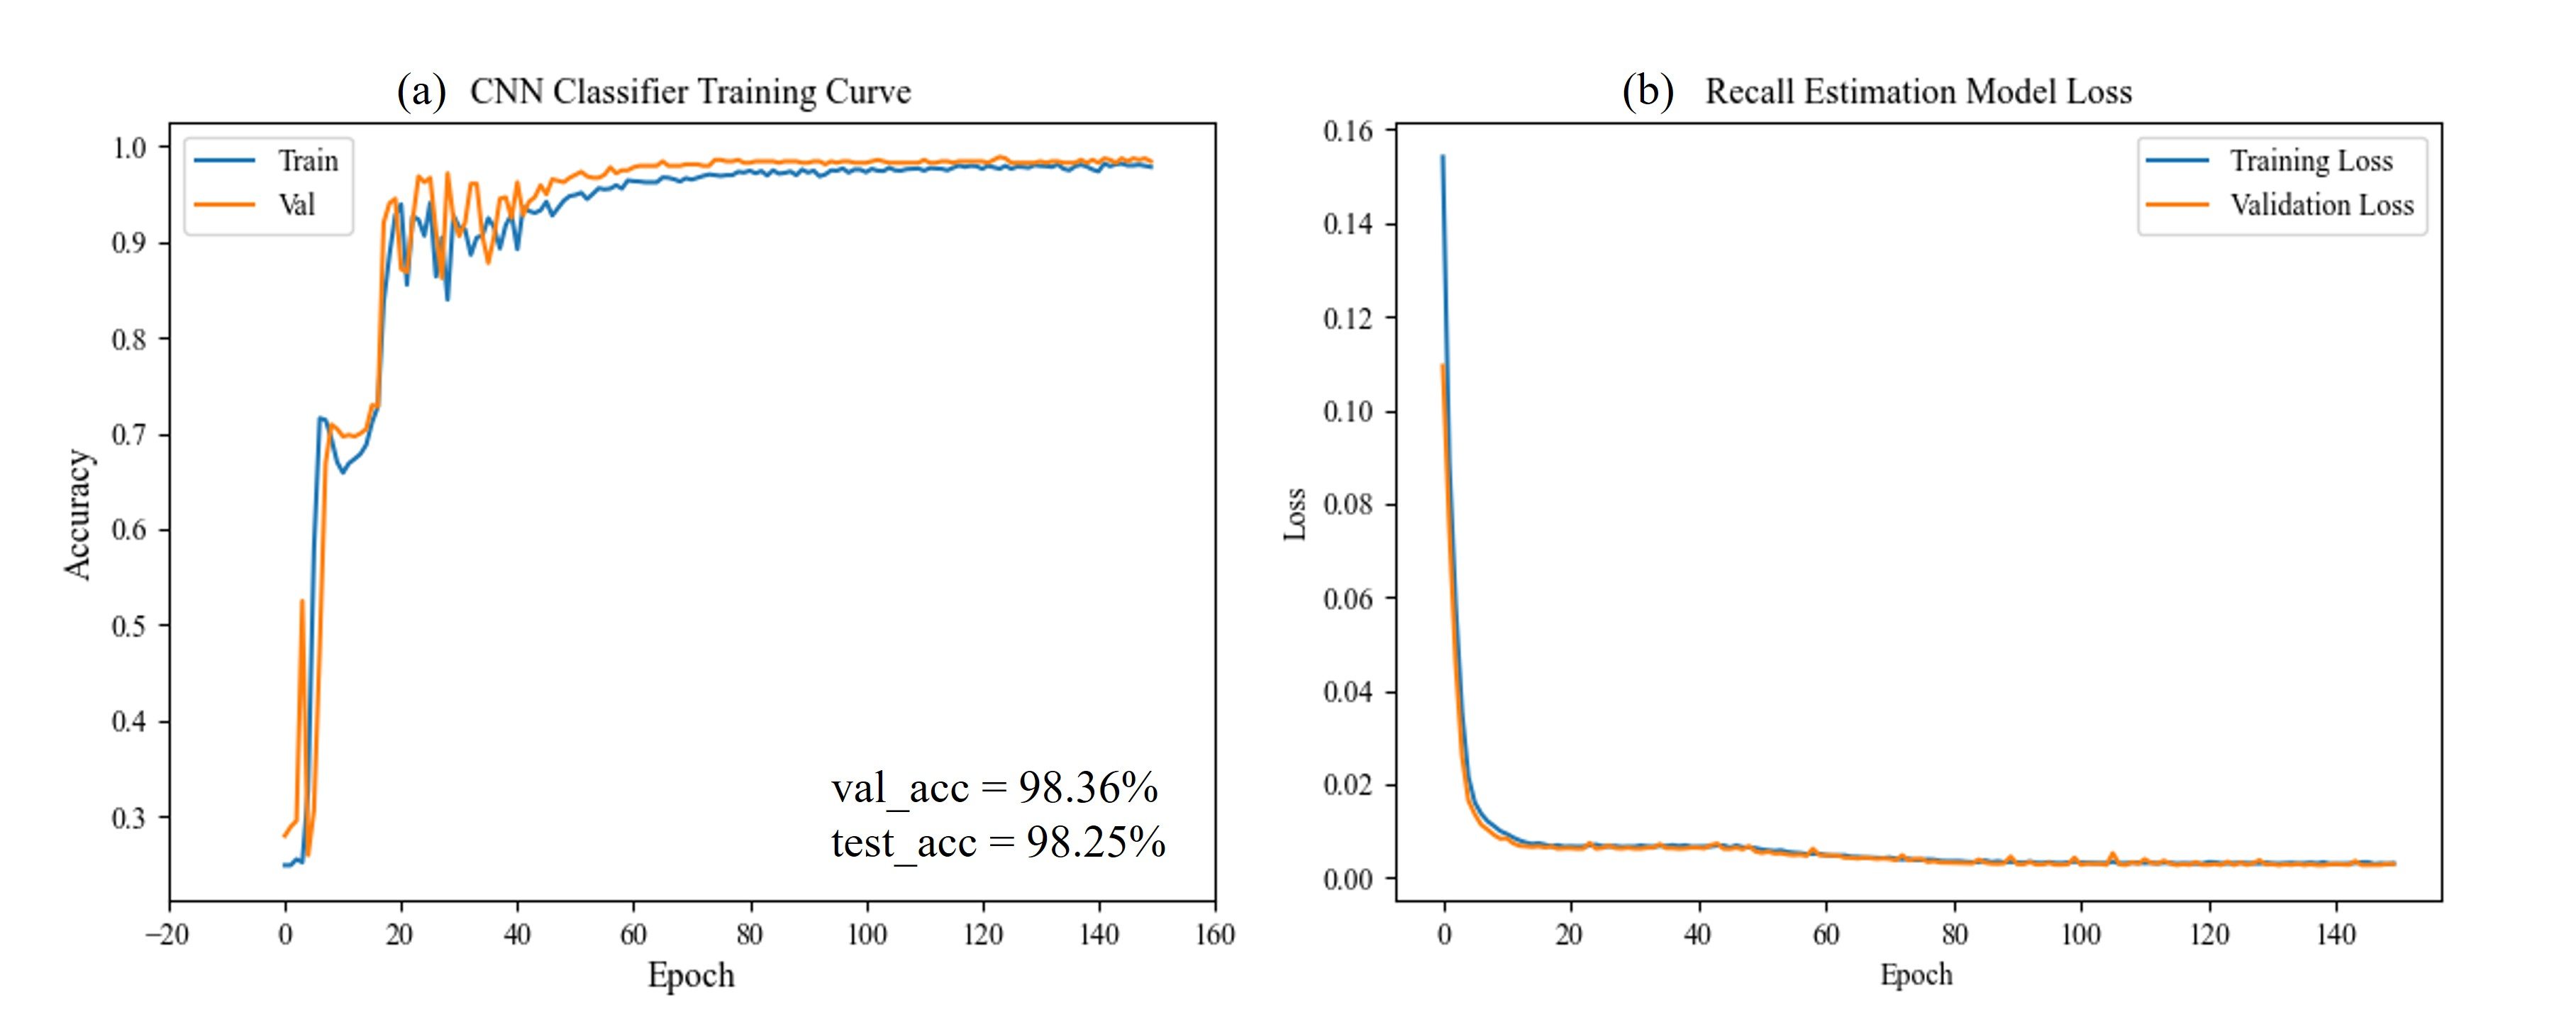
\includegraphics[width=\linewidth]{Fig14.jpg}
    \caption{Neural network training results: (a) CNN training results, (b) DNN training results.}
    \label{fig: NN Training Results}
\end{figure}

\subsubsection{Stage I: pre-deployment optimization}

As discussed in Section \ref{sec:digital_twin_pre-optimization} and illustrated in Figure \ref{fig:Edge Deployment Strategy} (a), the pre-deployment optimization stage comprises three key tasks leveraging the digital twin for signal generation:
(1) surrogate model pre-optimization,
(2) artificial dataset generation for real-world fine-tuning, and
(3) neural network training. To standardize evaluation, event signal generation in this study follows a unified setup with a 60-second duration and a 100 Hz sampling rate, assuming at most one event of interest per signal clip.

The first task requires seamless transferability to real-world scenarios. To achieve this, the noise level must be calibrated to a realistic value, while the event distribution remains flexible. Before signal generation, a preliminary sensing campaign is conducted to capture real-world ambient vibration data, which is then used to calibrate the noise level in the digital twin, as shown in Figures \ref{fig:Signal Synthesizing} (a) and (b). For each type of event of interest, 200 signal clips were generated, totaling 600 clips. Accordingly, the number of events of no interest, i.e., ambient vibration, was set to 600, ensuring a balanced dataset for surrogate model training, as shown in Figure \ref{fig:Signal Synthesizing} (b). This task is actually the first stage for the Bayesian optimization, and for initial observation, 15 points were randomly sampled from the search space spanned by threshold and duration. The threshold ranges from 0 to maximum amplitude of the ambient vibration captured by pioneer sensing, and the duration ranges from 2 to 10. Afterwards, the surrogate model was trained on the dataset for 50 iterations to optimize the triggering parameters. Note that since Stage I is mainly for pre-optimization, the balance factor $\beta$ in the UCB acquisition function is set to 2 to encourage exploration in iteration as shown in Table \ref{tab:optimization-configuration}. Moreover, to accelerate the iteration, the samples with both precision and recall over 0.9 were given a bonus of 1.1. 

The second task aims to generate artificial datasets for real-world fine-tuning, which follows the same distribution as the one in the first task. One difference is that the ambient vibration for onboard optimization is replaced with real-world data as shown in Figure \ref{fig:Signal Synthesizing} (c), and the replacement is in fact carried out in Stage II. The other difference is the scale of the dataset, which is much smaller. More specifically, 50 signal clips are generated for each type of event of interest, and 150 clips for ambient vibration, totaling 300 clips.

In the third task, as shown in Figure \ref{fig:Signal Synthesizing} (d), the CNN is trained with a balanced dataset, of which each type of event has 1000 signal clips and examples are shown in Figure \ref{fig: Synthesized Data Example}. For DNN, it is not directly trained on the event signal dataset, but rather on a dataset of recall values calculated under different triggering thresholds, durations, and noise levels. To derive the recall value dataset, a dataset containing 200 signals of each type of event was generated, totaling 600 clips. This dataset was then mixed with ambient vibration data at varying noise levels to simulate real-world scenarios. Notably, before calculating recall values, a search space for triggering parameters and noise levels was defined, gridded with logarithmic scales to ensure comprehensive coverage, refer to Figure \ref{fig: DNN Training Dataset} and Table \ref{tab:optimization-configuration} for details. The training curves of the neural networks are shown in Figure \ref{fig: NN Training Results} and the confusion matrix for CNN can be found in Figure \ref{fig: CNN Confusion Matrix}.


\begin{table}[h!]
    \centering
    \caption{Optimization Configuration for Virtual Environment Optimization}
    \label{tab:optimization-configuration}
    \renewcommand{\arraystretch}{1.5}
    {\fontfamily{ptm}\selectfont % Times New Roman Start
    \small
    \begin{tabular}{|p{0.2\textwidth}|p{0.5\textwidth}|p{0.2\textwidth}|}
    \hline
    \textbf{Parameter}  & \textbf{Description}  & \textbf{Value}  \\ \hline
    Ambient Vibration Intensity & The noise level range (times to captured noise level), uniform distribution. & 0.9 to 1.1 \\ \hline
    Earthquake Peak Value & The amplitude of the maximum earthquake response, uniform distribution. & 0.1g to 3.0g \\ \hline
    Impact Peak Value & The amplitude of the maximum impact response, uniform distribution. & 0.1g to 3.0g \\ \hline
    Strong Wind Peak Value & The amplitude of the maximum strong wind response (times to maximum ambient vibration), uniform distribution. & 1.5 to 2.5 \\ \hline
    $\beta$ & The balance factor in Equation \ref{eq:F-beta}. & 5 \\ \hline
    $\alpha$ & The scaling factor in Equation \ref{eq:matern-2.5-kernel}. & 1 \\ \hline
    $\lambda$ & The length scale factor in Equation \ref{eq:matern-2.5-kernel}. & 1 \\ \hline
    $\sigma_n^2$ & The parameter $\sigma_n^2$ in Equation \ref{eq:marginal-likelihood}. & 0.1 \\ \hline
    Initial Observation Number & The number of initial observation points as described in Algorithm \ref{alg:SMBO}. & 15 \\ \hline
    Iteration Number of Virtual Optimization & The number of iterations for virtual environment optimization as described in Algorithm \ref{alg:SMBO}. & 50 \\ \hline
    Iteration Number of Real-world Optimization & The number of iterations for real-world optimization as described in Algorithm \ref{alg:SMBO}. & 20 \\ \hline
    $\beta_{ucb1}$ & Parameter $\beta$ in UCB acquisition function to balance exploitation and exploration. (pre-optimization stage) & 2 \\ \hline
    $\beta_{ucb2}$ & Parameter $\beta$ in UCB acquisition function to balance exploitation and exploration. (onboard deployment stage) & 0.5 \\ \hline
    $f_{bonux}$ & Bonus factor for F-beta score when precision and recall are higher than 0.9. & 1.1 \\ \hline
    $t_{lb}$ & lower bound for triggering threshold. & 0 \\ \hline
    $t_{ub}$ & upper bound for triggering threshold (twice the average absolute amplitude of the ambient vibration or the noise). & 0.01706 \\ \hline
    $d_{lb}$ & lower bound for triggering duration, integer & 2 \\ \hline
    $d_{ub}$ & upper bound for triggering duration, integer & 10 \\ \hline
    \end{tabular}
    } % Times New Roman End
\end{table}

\subsubsection{Stage II: onboard optimization}

In Stage II, the pre-optimized surrogate model, triggering parameters, synthesized dataset, and neural networks are deployed to the edge device for real world fine-tuning. The validation is performed on a LiftNode powered by ESP32 MCU, featuring official support for signal processing (ESP-DSP) and deep learning (ESP-DL). Moreover, LiftNode is equipped with TinySHM, a distributed edge intelligence enabling framework also developed by LIFT at NTU for IoT-based SHM, to facilitate signal processing and AI deployment.

For dataset processing, the synthesized event of interest signals were first stored onboard, using TF card storage. Afterwards, the ambient vibration data was automatically captured by programming and then stored in the same TF card to mix with the previously stored event of interest signals to form the dataset for real world fine-tuning as shown in Figure \ref{fig:Signal Synthesizing} (c). Note that the data captured was first calibrated by removing the mean value obtained from the pioneer sensing before downstream signal processing.

\subsection{Smart adaptive trigger sensing results}

\begin{figure}[htbp]
    \centering
    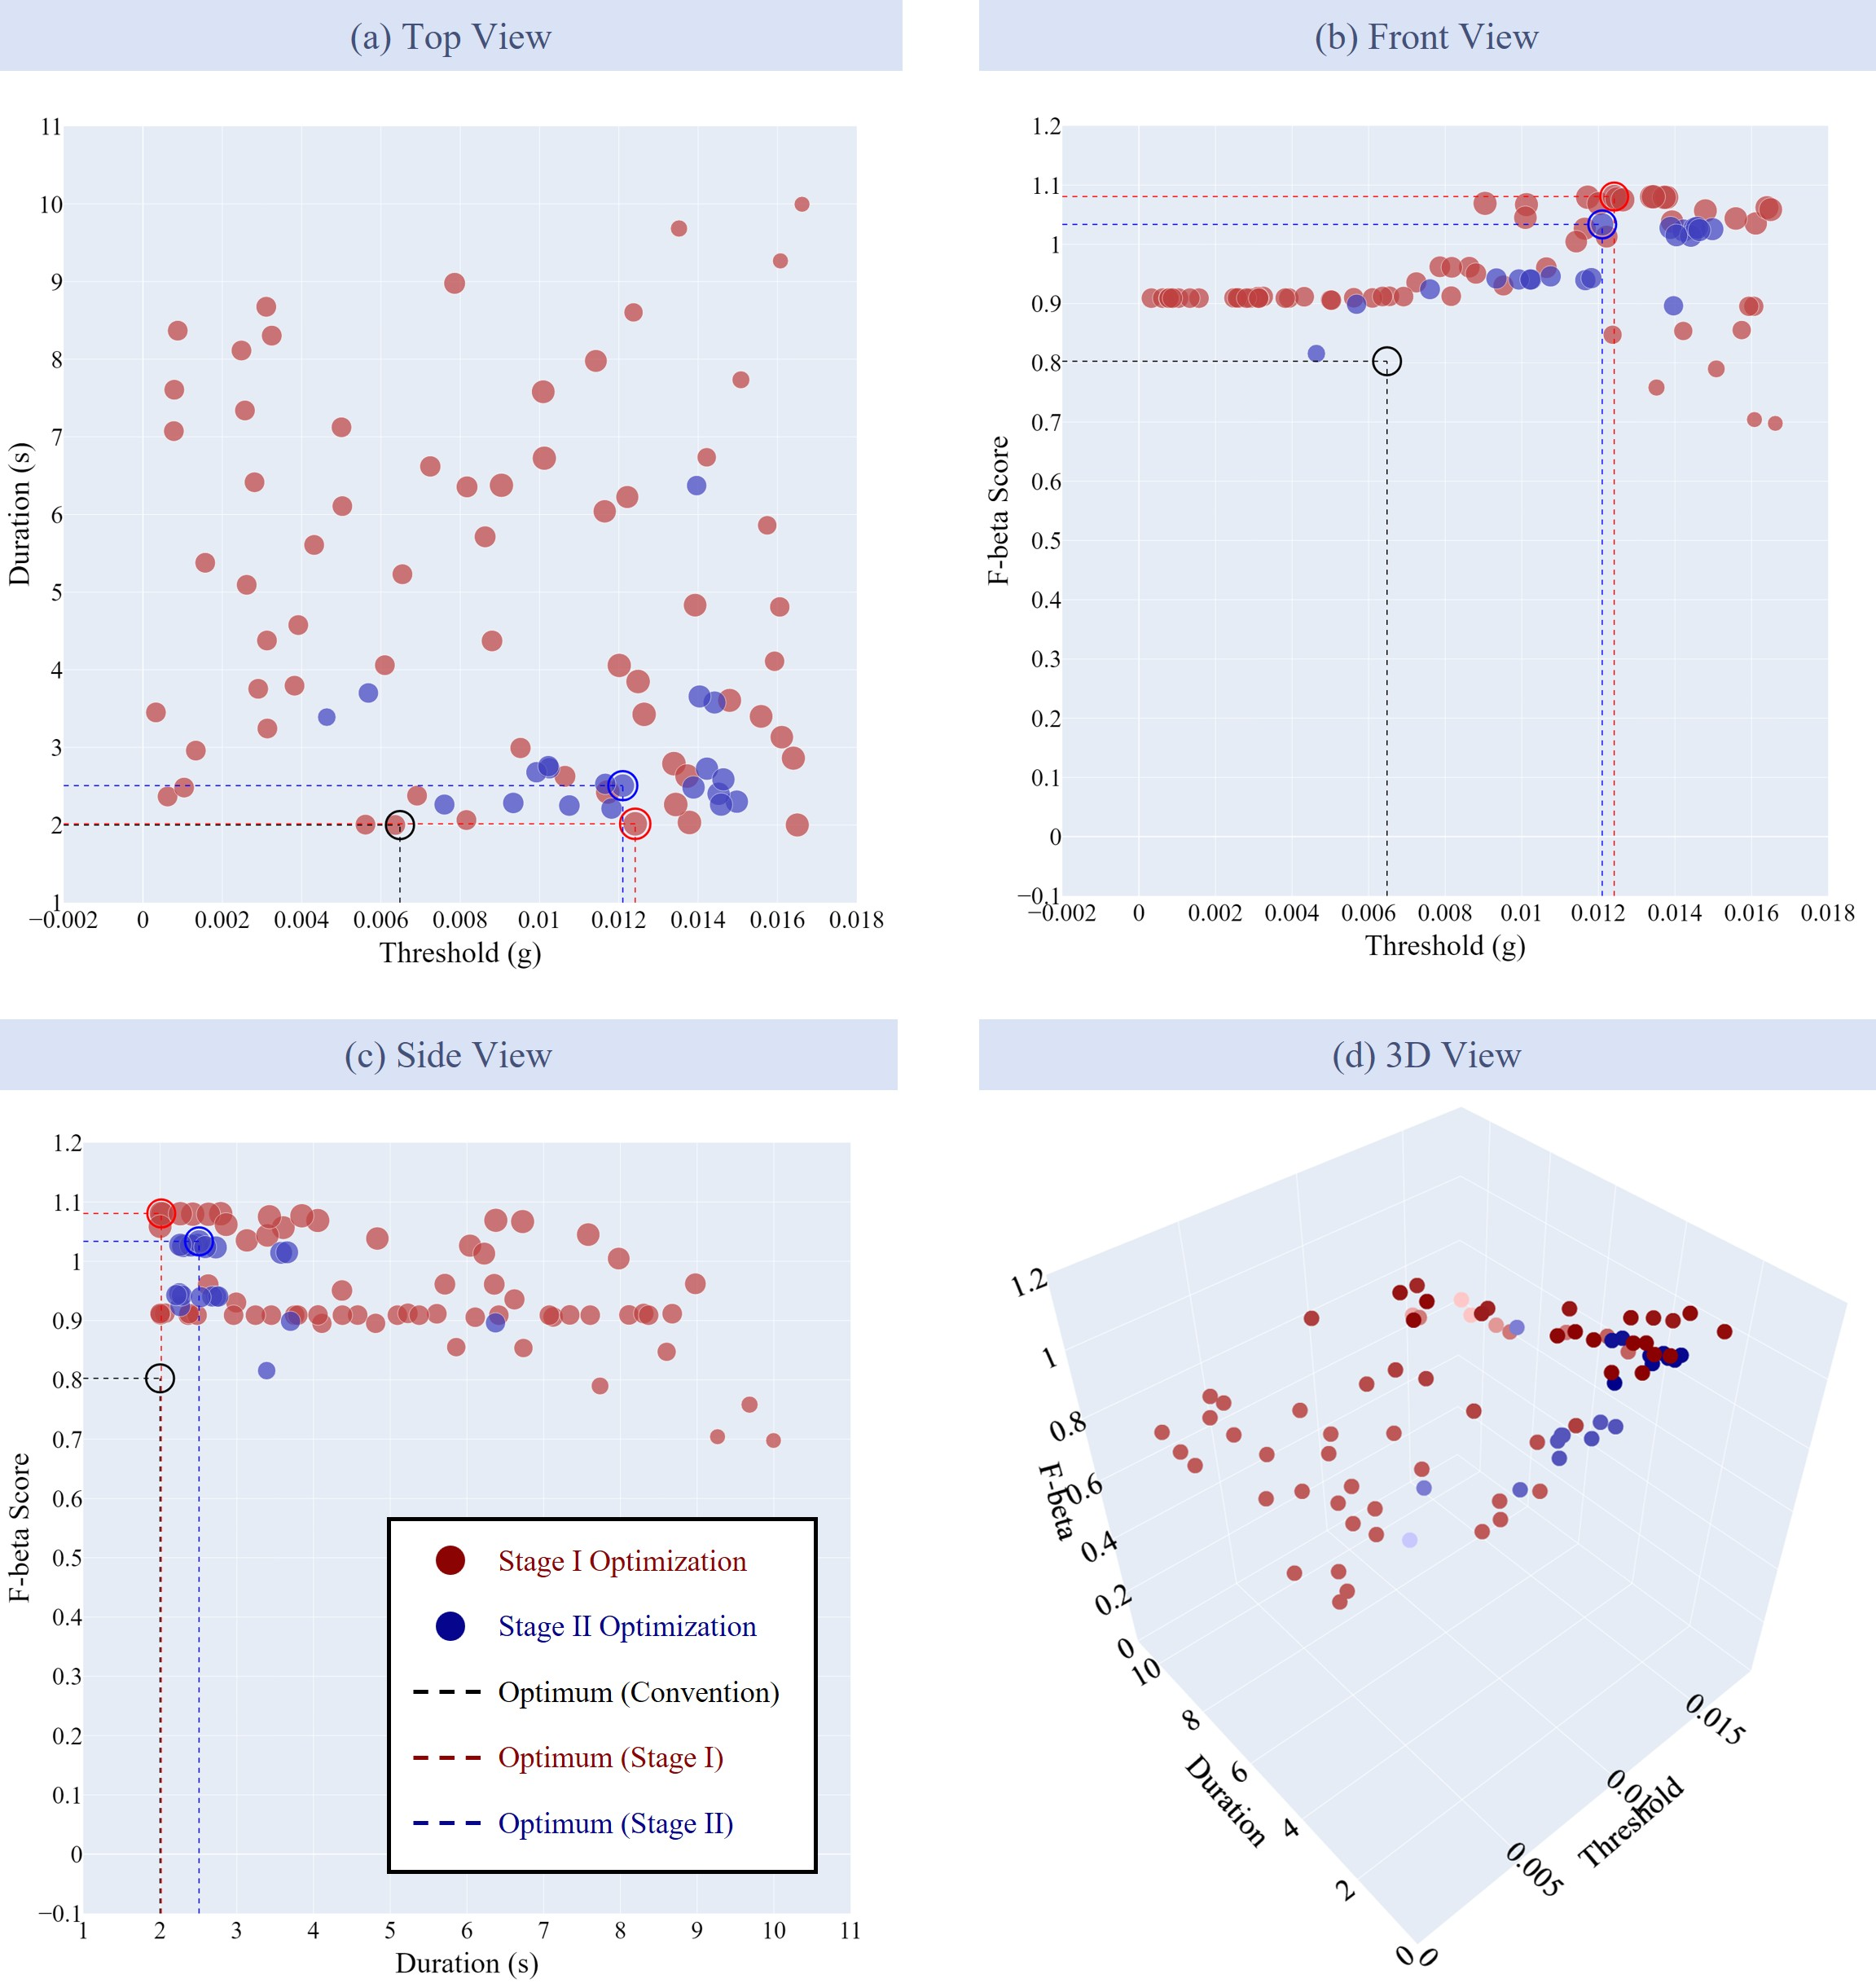
\includegraphics[width=\linewidth]{Fig15.jpg}
    \caption{Laboratory test results: (a) top view, (b) front view, (c) side view, (d) 3D view.}
    \label{fig:Lab Test Results}
\end{figure}

To evaluate the performance of the proposed SATM, the conventional way, i.e., `pioneer sensing + manual parameter setup', is first evaluated. Based on the pioneer sensing results, mainly for ambient vibration, to avoid missing important events, the triggering parameter was conservatively set to 0.00648g which is twice the standard deviation of the ambient vibration captured in pioneer sensing. The duration is set to 2 sampling points. As marked in Figure \ref{fig:Lab Test Results} by black circle and dash lines, the conventional method can achieve a $F_{\beta}$ score of 0.8025, which serves as the baseline for comparison. The corresponding recall is 100\% and precision is only 50\%. This setup demonstrates a common conservative tendency in SHM practice, which can lead to a high recall but sacrifices precision.

The results of the proposed SATM are comprehensively given by Table \ref{tab:comparison} and Figures \ref{fig:Lab Test Results} and \ref{fig:Metric History}. Table \ref{tab:comparison} quantitatively compares the conventional method performance with the proposed SATM method, which is further broken down into Stage I and Stage II for better insights. Figures \ref{fig:Lab Test Results} and \ref{fig:Metric History} provide visual representations of the results, with Figure \ref{fig:Lab Test Results} showing the spatial positions in the searching space and the Figure \ref{fig:Metric History} showing the iteration history of the optimization process in sequential order. The associated precision and recall values are also given in Figure \ref{fig:Metric History}.

\begin{figure}[htbp]
    \centering
    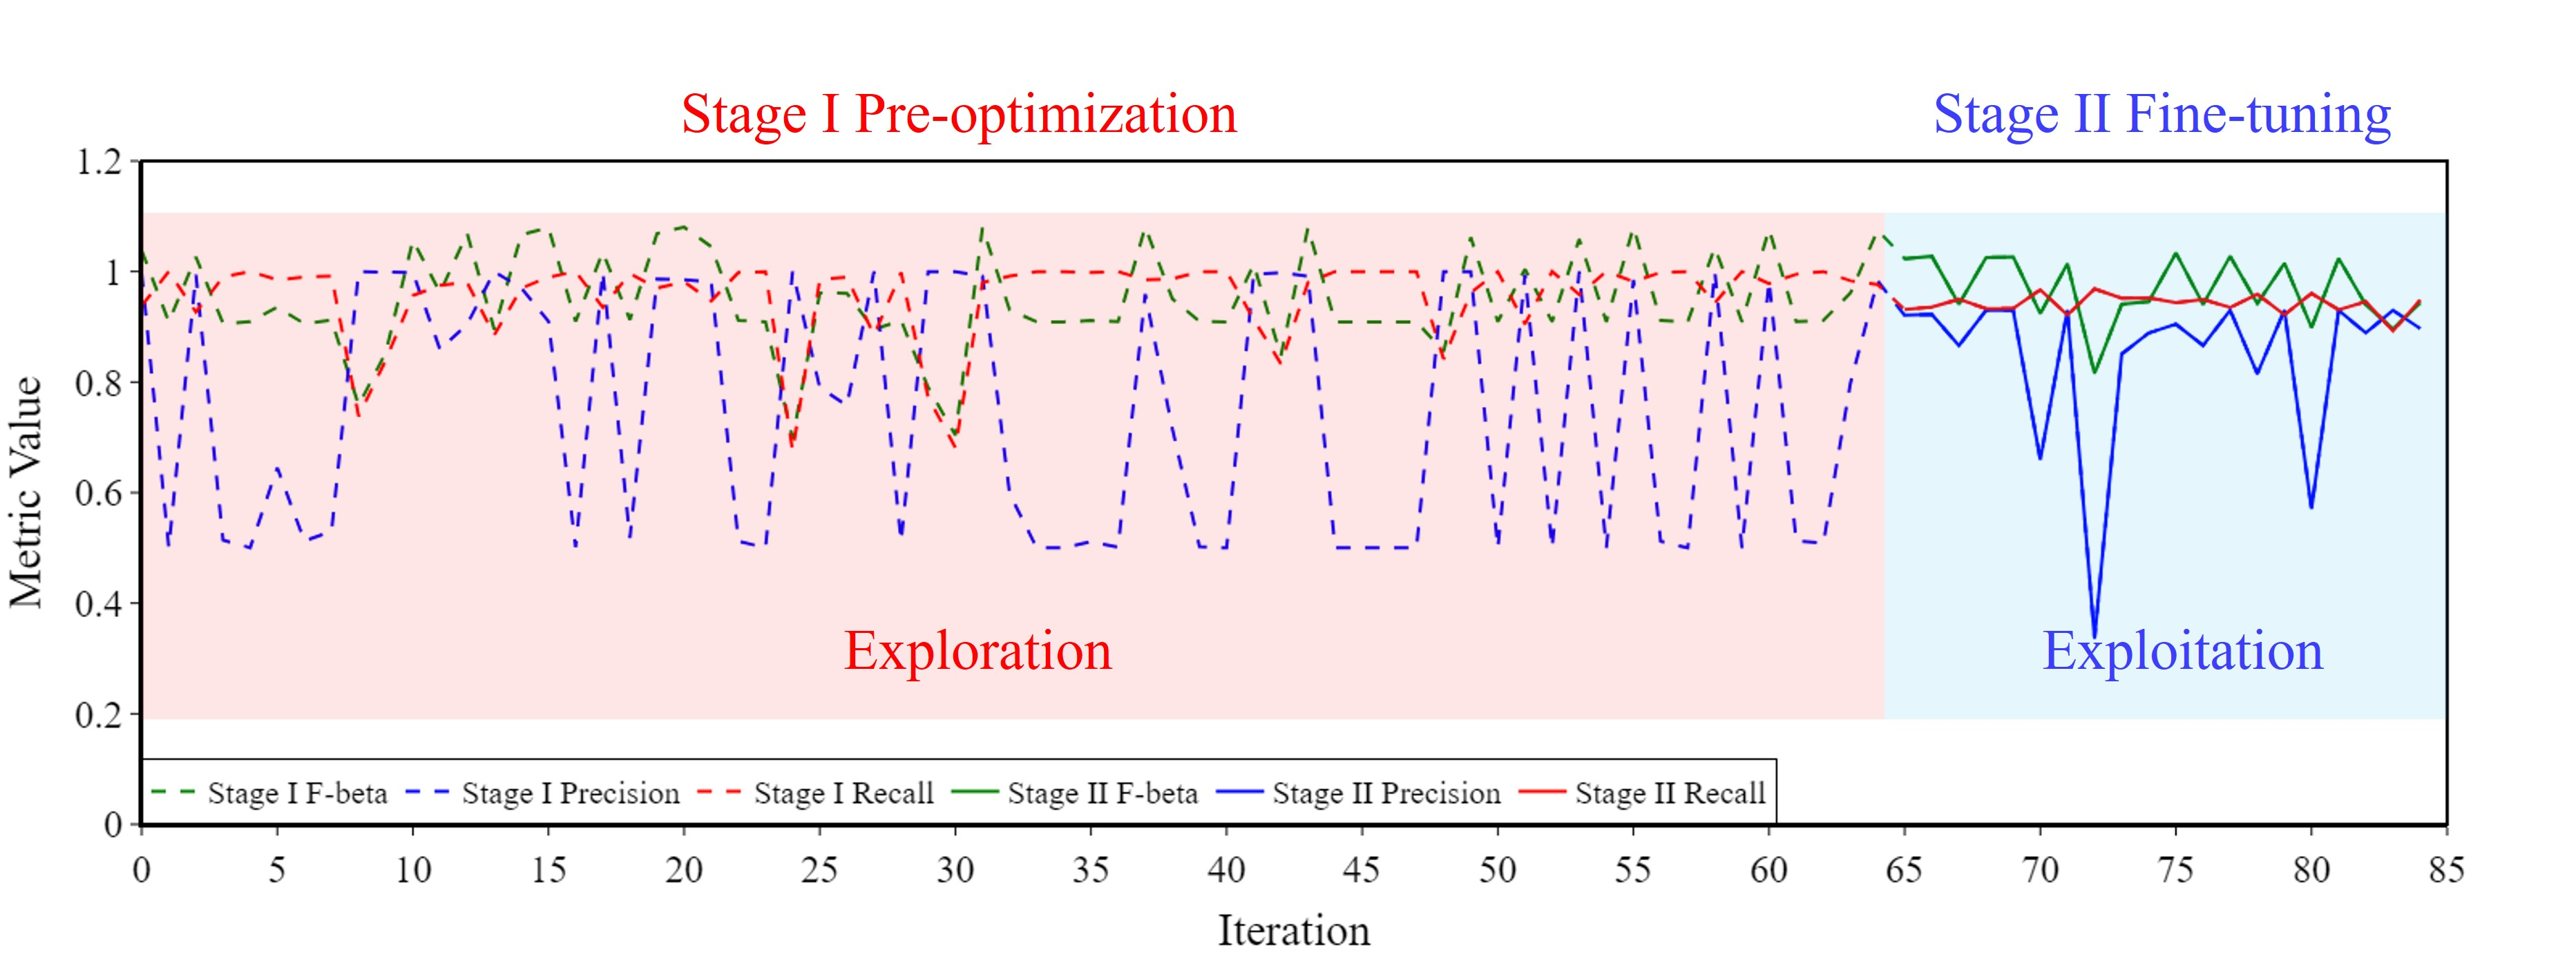
\includegraphics[width=\linewidth]{Fig16.jpg}
    \caption{Time history of metrics during optimization iteration.}
    \label{fig:Metric History}
\end{figure}

\begin{table}[h!]
    \centering
    \caption{Comparison of the conventional method and the proposed SATM}
    \label{tab:comparison}
    \renewcommand{\arraystretch}{1.5}
    {\fontfamily{ptm}\selectfont % Times New Roman Start
    \small
    \begin{tabular}{|p{0.3\textwidth}|p{0.2\textwidth}|p{0.2\textwidth}|p{0.2\textwidth}|}
    \hline
    \textbf{Item}  & \textbf{$F_{\beta}$}  & \textbf{Precision} & \textbf{Recall}\\ \hline
    Conventional Setup & 0.8025 & 50\% & 100\% \\ \hline
    Stage I Pre-optimization & 1.0806 & 95.94\% & 98.50\% \\ \hline
    Stage II Onboard Fine-tuning & 1.0336 & 90.48\% & 94.36\% \\ \hline
    \end{tabular}
    } % Times New Roman End
\end{table}

As revealed by the results, the following observations and conclusions can be drawn:

\begin{enumerate}[a)]
    \item The proposed SATM significantly outperforms the conventional method, achieving an \(F_{\beta}\) score of 1.0806 in pre-optimization and 1.0336 in onboard optimization, compared to 0.8025 for the conventional approach. This clearly demonstrates the effectiveness of SATM in optimizing triggering parameters for SHM applications.
    \item The data distributions observed in both pre-optimization (via the digital twin) and onboard optimization are highly similar, indicating excellent transferability from synthetic to real-world scenarios. Although some discrepancies exist due to inherent differences between artificial and real data, these are expected to diminish as more real-world data becomes available and accumulates.
    \item The surrogate model, well-trained within the digital twin environment, enables onboard fine-tuning to converge in significantly fewer iterations than pre-optimization. This efficiency is reflected in both the rapid convergence toward high-scoring configurations and the higher average performance achieved during onboard optimization.
    \item The two-stage deployment strategy effectively balances exploration and exploitation: the first stage, focused on exploration, exhibits larger metric fluctuations to thoroughly search the parameter space, while the second stage exploits the gathered knowledge to refine the configuration, resulting in a robust and optimized system performance.
\end{enumerate}

\section{Conclusion}
\label{sec:conclusion}

This study proposes a smart adaptive triggering mechanism that synergistically integrates feedback loop control, digital twin technology, and Bayesian optimization. Designed to address challenges including limited adaptivity, multi-objective optimization, unknown event distributions, absence of ground truth, partial observability, and high observation costs, the SATM comprises four fundamental components: the environment, system, estimator, and controller. The mechanism operates in two distinct phases: first, a digital twin-based pre-optimization phase to establish a good initial configuration, followed by an onboard fine-tuning phase to refine parameters under real-world conditions. Laboratory experiments demonstrate that the SATM effectively optimizes triggering parameters, yielding real-world performance improvements around 30\% in the \(F_{\beta}\) score relative to conventional methods. Overall, the SATM exhibits significant potential for enabling automatic and adaptive parameter adjustments in trigger sensing applications across diverse industries.

\section*{Acknowledgements}
\label{sec:acknowledgements}

The authors want to gratefully acknowledge the financial support of this research from NTU Start-up Grant 03INS001210C120 and MOE AcRF Tier 1 Grants, No. RG121/21.

\section*{Declaration of generative AI and AI-assisted technologies in the writing process}
\label{sec:declaration}
During the preparation of this work the authors used ChatGPT in order to improve the readability and language of the manuscript. After using this tool/service, the authors reviewed and edited the content as needed and take full responsibility for the content of the published article.

\section*{Appendices}

For code details, please refer to the GitHub repositories below.

Excitation-Structure-Response Simulation: 

\url{https://github.com/Shuaiwen-Cui/Research-Excitation_Structure_Response.git}

Smart Adaptive Trigger Sensing: 

\url{https://github.com/Shuaiwen-Cui/Research-Smart\_Adaptive\_Trigger\_Sensing.git}

% Numbered list
% Use the style of numbering in square brackets.
% If nothing is used, default style will be taken.
%\begin{enumerate}[a)]
%\item 
%\item 
%\item 
%\end{enumerate}  

% Unnumbered list
%\begin{itemize}
%\item 
%\item 
%\item 
%\end{itemize}  

% Description list
%\begin{description}
%\item[]
%\item[] 
%\item[] 
%\end{description}  

% Figure
% \begin{figure}[<options>]
% 	\centering
% 		\includegraphics[<options>]{}
% 	  \caption{}\label{fig1}
% \end{figure}


% \begin{table}[<options>]
% \caption{}\label{tbl1}
% \begin{tabular*}{\tblwidth}{@{}LL@{}}
% \toprule
%   &  \\ % Table header row
% \midrule
%  & \\
%  & \\
%  & \\
%  & \\
% \bottomrule
% \end{tabular*}
% \end{table}

% Uncomment and use as the case may be
%\begin{theorem} 
%\end{theorem}

% Uncomment and use as the case may be
%\begin{lemma} 
%\end{lemma}

%% The Appendices part is started with the command \appendix;
%% appendix sections are then done as normal sections
%% \appendix

% To print the credit authorship contribution details
% \printcredits

%% Loading bibliography style file
% \bibliographystyle{model1-num-names}
% \bibliographystyle{cas-model2-names}
% \bibliographystyle{unsrt}
\bibliographystyle{elsarticle-num}

% Loading bibliography database
\bibliography{ref}

% Biography
% \bio{}
% Here goes the biography details.
% \endbio

% \bio{pic1}
% Here goes the biography details.
% \endbio

\end{document}

